% Options for packages loaded elsewhere
% Options for packages loaded elsewhere
\PassOptionsToPackage{unicode}{hyperref}
\PassOptionsToPackage{hyphens}{url}
\PassOptionsToPackage{dvipsnames,svgnames,x11names}{xcolor}
%
\documentclass[
  letterpaper,
  DIV=11,
  numbers=noendperiod]{scrreprt}
\usepackage{xcolor}
\usepackage{amsmath,amssymb}
\setcounter{secnumdepth}{5}
\usepackage{iftex}
\ifPDFTeX
  \usepackage[T1]{fontenc}
  \usepackage[utf8]{inputenc}
  \usepackage{textcomp} % provide euro and other symbols
\else % if luatex or xetex
  \usepackage{unicode-math} % this also loads fontspec
  \defaultfontfeatures{Scale=MatchLowercase}
  \defaultfontfeatures[\rmfamily]{Ligatures=TeX,Scale=1}
\fi
\usepackage{lmodern}
\ifPDFTeX\else
  % xetex/luatex font selection
\fi
% Use upquote if available, for straight quotes in verbatim environments
\IfFileExists{upquote.sty}{\usepackage{upquote}}{}
\IfFileExists{microtype.sty}{% use microtype if available
  \usepackage[]{microtype}
  \UseMicrotypeSet[protrusion]{basicmath} % disable protrusion for tt fonts
}{}
\makeatletter
\@ifundefined{KOMAClassName}{% if non-KOMA class
  \IfFileExists{parskip.sty}{%
    \usepackage{parskip}
  }{% else
    \setlength{\parindent}{0pt}
    \setlength{\parskip}{6pt plus 2pt minus 1pt}}
}{% if KOMA class
  \KOMAoptions{parskip=half}}
\makeatother
% Make \paragraph and \subparagraph free-standing
\makeatletter
\ifx\paragraph\undefined\else
  \let\oldparagraph\paragraph
  \renewcommand{\paragraph}{
    \@ifstar
      \xxxParagraphStar
      \xxxParagraphNoStar
  }
  \newcommand{\xxxParagraphStar}[1]{\oldparagraph*{#1}\mbox{}}
  \newcommand{\xxxParagraphNoStar}[1]{\oldparagraph{#1}\mbox{}}
\fi
\ifx\subparagraph\undefined\else
  \let\oldsubparagraph\subparagraph
  \renewcommand{\subparagraph}{
    \@ifstar
      \xxxSubParagraphStar
      \xxxSubParagraphNoStar
  }
  \newcommand{\xxxSubParagraphStar}[1]{\oldsubparagraph*{#1}\mbox{}}
  \newcommand{\xxxSubParagraphNoStar}[1]{\oldsubparagraph{#1}\mbox{}}
\fi
\makeatother


\usepackage{longtable,booktabs,array}
\usepackage{calc} % for calculating minipage widths
% Correct order of tables after \paragraph or \subparagraph
\usepackage{etoolbox}
\makeatletter
\patchcmd\longtable{\par}{\if@noskipsec\mbox{}\fi\par}{}{}
\makeatother
% Allow footnotes in longtable head/foot
\IfFileExists{footnotehyper.sty}{\usepackage{footnotehyper}}{\usepackage{footnote}}
\makesavenoteenv{longtable}
\usepackage{graphicx}
\makeatletter
\newsavebox\pandoc@box
\newcommand*\pandocbounded[1]{% scales image to fit in text height/width
  \sbox\pandoc@box{#1}%
  \Gscale@div\@tempa{\textheight}{\dimexpr\ht\pandoc@box+\dp\pandoc@box\relax}%
  \Gscale@div\@tempb{\linewidth}{\wd\pandoc@box}%
  \ifdim\@tempb\p@<\@tempa\p@\let\@tempa\@tempb\fi% select the smaller of both
  \ifdim\@tempa\p@<\p@\scalebox{\@tempa}{\usebox\pandoc@box}%
  \else\usebox{\pandoc@box}%
  \fi%
}
% Set default figure placement to htbp
\def\fps@figure{htbp}
\makeatother


% definitions for citeproc citations
\NewDocumentCommand\citeproctext{}{}
\NewDocumentCommand\citeproc{mm}{%
  \begingroup\def\citeproctext{#2}\cite{#1}\endgroup}
\makeatletter
 % allow citations to break across lines
 \let\@cite@ofmt\@firstofone
 % avoid brackets around text for \cite:
 \def\@biblabel#1{}
 \def\@cite#1#2{{#1\if@tempswa , #2\fi}}
\makeatother
\newlength{\cslhangindent}
\setlength{\cslhangindent}{1.5em}
\newlength{\csllabelwidth}
\setlength{\csllabelwidth}{3em}
\newenvironment{CSLReferences}[2] % #1 hanging-indent, #2 entry-spacing
 {\begin{list}{}{%
  \setlength{\itemindent}{0pt}
  \setlength{\leftmargin}{0pt}
  \setlength{\parsep}{0pt}
  % turn on hanging indent if param 1 is 1
  \ifodd #1
   \setlength{\leftmargin}{\cslhangindent}
   \setlength{\itemindent}{-1\cslhangindent}
  \fi
  % set entry spacing
  \setlength{\itemsep}{#2\baselineskip}}}
 {\end{list}}
\usepackage{calc}
\newcommand{\CSLBlock}[1]{\hfill\break\parbox[t]{\linewidth}{\strut\ignorespaces#1\strut}}
\newcommand{\CSLLeftMargin}[1]{\parbox[t]{\csllabelwidth}{\strut#1\strut}}
\newcommand{\CSLRightInline}[1]{\parbox[t]{\linewidth - \csllabelwidth}{\strut#1\strut}}
\newcommand{\CSLIndent}[1]{\hspace{\cslhangindent}#1}



\setlength{\emergencystretch}{3em} % prevent overfull lines

\providecommand{\tightlist}{%
  \setlength{\itemsep}{0pt}\setlength{\parskip}{0pt}}



 


\def\R{\mathbb R}
\def\N{\mathbb N}
\def\Q{\mathbb Q}
\def\Z{\mathbb Z}
\newcommand{\st}{~:~}
\newcommand{\cee}{\mathsf{C}}
\newcommand{\bee}{\mathrm{B}}
\KOMAoption{captions}{tableheading}
\makeatletter
\@ifpackageloaded{float}{}{\usepackage{float}}
\floatstyle{plain}
\@ifundefined{c@chapter}{\newfloat{desmos}{h}{lodes}}{\newfloat{desmos}{h}{lodes}[chapter]}
\floatname{desmos}{Desmos Applet}
\newcommand*\listofdesmoss{\listof{desmos}{List of Desmos Applets}}
\makeatother
\makeatletter
\@ifpackageloaded{tcolorbox}{}{\usepackage[skins,breakable]{tcolorbox}}
\@ifpackageloaded{fontawesome5}{}{\usepackage{fontawesome5}}
\definecolor{quarto-callout-color}{HTML}{909090}
\definecolor{quarto-callout-note-color}{HTML}{0758E5}
\definecolor{quarto-callout-important-color}{HTML}{CC1914}
\definecolor{quarto-callout-warning-color}{HTML}{EB9113}
\definecolor{quarto-callout-tip-color}{HTML}{00A047}
\definecolor{quarto-callout-caution-color}{HTML}{FC5300}
\definecolor{quarto-callout-color-frame}{HTML}{acacac}
\definecolor{quarto-callout-note-color-frame}{HTML}{4582ec}
\definecolor{quarto-callout-important-color-frame}{HTML}{d9534f}
\definecolor{quarto-callout-warning-color-frame}{HTML}{f0ad4e}
\definecolor{quarto-callout-tip-color-frame}{HTML}{02b875}
\definecolor{quarto-callout-caution-color-frame}{HTML}{fd7e14}
\makeatother
\makeatletter
\@ifpackageloaded{bookmark}{}{\usepackage{bookmark}}
\makeatother
\makeatletter
\@ifpackageloaded{caption}{}{\usepackage{caption}}
\AtBeginDocument{%
\ifdefined\contentsname
  \renewcommand*\contentsname{Table of contents}
\else
  \newcommand\contentsname{Table of contents}
\fi
\ifdefined\listfigurename
  \renewcommand*\listfigurename{List of Figures}
\else
  \newcommand\listfigurename{List of Figures}
\fi
\ifdefined\listtablename
  \renewcommand*\listtablename{List of Tables}
\else
  \newcommand\listtablename{List of Tables}
\fi
\ifdefined\figurename
  \renewcommand*\figurename{Figure}
\else
  \newcommand\figurename{Figure}
\fi
\ifdefined\tablename
  \renewcommand*\tablename{Table}
\else
  \newcommand\tablename{Table}
\fi
}
\@ifpackageloaded{float}{}{\usepackage{float}}
\floatstyle{ruled}
\@ifundefined{c@chapter}{\newfloat{codelisting}{h}{lop}}{\newfloat{codelisting}{h}{lop}[chapter]}
\floatname{codelisting}{Listing}
\newcommand*\listoflistings{\listof{codelisting}{List of Listings}}
\usepackage{amsthm}
\theoremstyle{definition}
\newtheorem{example}{Example}[chapter]
\theoremstyle{plain}
\newtheorem{lemma}{Lemma}[chapter]
\theoremstyle{definition}
\newtheorem{exercise}{Exercise}[chapter]
\theoremstyle{definition}
\newtheorem{definition}{Definition}[chapter]
\theoremstyle{plain}
\newtheorem{theorem}{Theorem}[chapter]
\theoremstyle{plain}
\newtheorem{corollary}{Corollary}[chapter]
\theoremstyle{remark}
\AtBeginDocument{\renewcommand*{\proofname}{Proof}}
\newtheorem*{remark}{Remark}
\newtheorem*{solution}{Solution}
\newtheorem{refremark}{Remark}[chapter]
\newtheorem{refsolution}{Solution}[chapter]
\makeatother
\makeatletter
\makeatother
\makeatletter
\@ifpackageloaded{caption}{}{\usepackage{caption}}
\@ifpackageloaded{subcaption}{}{\usepackage{subcaption}}
\makeatother
\usepackage{bookmark}
\IfFileExists{xurl.sty}{\usepackage{xurl}}{} % add URL line breaks if available
\urlstyle{same}
\hypersetup{
  pdftitle={Real Analysis},
  pdfauthor={Stepan Paul},
  colorlinks=true,
  linkcolor={blue},
  filecolor={Maroon},
  citecolor={Blue},
  urlcolor={Blue},
  pdfcreator={LaTeX via pandoc}}


\title{Real Analysis}
\author{Stepan Paul}
\date{2026-03-05}
\begin{document}
\maketitle

\makeatletter
\@ifundefined{c@proposition}{}{\@ifundefined{c@theorem}{}{\let\c@proposition\c@theorem\let\theproposition\thetheorem}}
\@ifundefined{c@lemma}{}{\@ifundefined{c@theorem}{}{\let\c@lemma\c@theorem\let\thelemma\thetheorem}}
\@ifundefined{c@definition}{}{\@ifundefined{c@theorem}{}{\let\c@definition\c@theorem\let\thedefinition\thetheorem}}
\@ifundefined{c@example}{}{\@ifundefined{c@theorem}{}{\let\c@example\c@theorem\let\theexample\thetheorem}}
\@ifundefined{c@exercise}{}{\@ifundefined{c@theorem}{}{\let\c@exercise\c@theorem\let\theexercise\thetheorem}}
\@ifundefined{c@problem}{}{\@ifundefined{c@theorem}{}{\let\c@problem\c@theorem\let\theproblem\thetheorem}}
\@ifundefined{c@corollary}{}{\@ifundefined{c@theorem}{}{\let\c@corollary\c@theorem\let\thecorollary\thetheorem}}
\makeatother

\renewcommand*\contentsname{Table of contents}
{
\hypersetup{linkcolor=}
\setcounter{tocdepth}{2}
\tableofcontents
}

\bookmarksetup{startatroot}

\chapter*{Preface}\label{preface}
\addcontentsline{toc}{chapter}{Preface}

\markboth{Preface}{Preface}

This is a Quarto book.

To learn more about Quarto books visit
\url{https://quarto.org/docs/books}.

\bookmarksetup{startatroot}

\chapter{Introduction}\label{introduction}

This is a book created from markdown and executable code.

See Knuth (1984) for additional discussion of literate programming.

\begin{theorem}[Fermat's First
Theorem]\protect\hypertarget{thm-hi}{}\label{thm-hi}

This extension has been written by a teacher who hopes that students
read the course notes\ldots{}

\end{theorem}

Please look back to Theorem~\ref{thm-hi}

\begin{lemma}[]\protect\hypertarget{lem-bye}{}\label{lem-bye}

This extension has been written by a teacher who hopes that students
read the course notes\ldots{}

\end{lemma}

\begin{exercise}[]\protect\hypertarget{exr-next}{}\label{exr-next}

This extension has been written by a teacher who hopes that students
read the course notes\ldots{}

\end{exercise}

\begin{example}[]\protect\hypertarget{exm-the}{}\label{exm-the}

This extension has been written by a teacher who hopes that students
read the course notes\ldots{}

\end{example}

\section{Acknowledgements}\label{acknowledgements}

The author acknowledges support of the Institut Henri
Poincar\textquotesingle e (UAR 839 CNRS-Sorbonne
Universit\textquotesingle e), and LabEx CARMIN (ANR-10-LABX-59-01).

Also thank: John Rock, Yuri Sulyman, Desmos

\part{The Real Numbers}

As discussed in the introduction, our approach to real analysis will be
to start by laying out a set of axioms that we \emph{assume} are true
about the real number system \(\R\) and then \emph{prove} everything
else based upon this set of axioms.

In order to properly take this approach, we need a set of axioms that:

\begin{itemize}
\tightlist
\item
  contains enough information to let us prove everything there is to
  know about \(\R\) (all of calculus, for example),
\item
  is specific enough so that it distinguishes \(\R\) from other number
  systems, and
\item
  is as simple as possible
\end{itemize}

The purpose of the first bullet point is clear enough: if I don't assume
anything, I won't be able to prove anything.

The second bullet point about distinguishing \(\R\) from other number
systems is related, but deserves some explanation. Consider the
following proposition:

\begin{quote}
For every \(x>0\), there exists \(y\) such that \(y^2=x\).
\end{quote}

This is true if our universe is \(\R\) but false our universe is \(\Q\).
If our axioms for \(\R\) do not distinguish it from \(\Q\), we will have
no hope of proving such a propositon. In short, I want a set of axioms
that is true for \(\R\) \emph{but for no other number system}.

\begin{tcolorbox}[enhanced jigsaw, coltitle=black, left=2mm, bottomrule=.15mm, bottomtitle=1mm, breakable, leftrule=.75mm, opacityback=0, colbacktitle=quarto-callout-note-color!10!white, toptitle=1mm, opacitybacktitle=0.6, colback=white, colframe=quarto-callout-note-color-frame, arc=.35mm, title=\textcolor{quarto-callout-note-color}{\faInfo}\hspace{0.5em}{Note}, titlerule=0mm, rightrule=.15mm, toprule=.15mm]

I am using the term \emph{number system} a bit loosely. For our
purposes, though, it's fine to think of any set with binary operations
corresponding to addition and multiplication---think
\(\mathbb{N},\mathbb{Z},\mathbb{Q},\mathbb{R},\mathbb{C}\).

\end{tcolorbox}

\section*{Notes}\label{notes}
\addcontentsline{toc}{section}{Notes}

\markright{Notes}

\begin{itemize}
\tightlist
\item
  Should include an thought experiment about how do we know there is a
  number \(x\) such that \(e^x+x=1\) (with Desmos graphic).
\item
  Should include something about how mathematics shifted from a search
  for absolute truth to a search for understanding of how consequences
  follow from hypotheses.
\end{itemize}

\chapter{The Field and Order Axioms}\label{the-field-and-order-axioms}

\section{Highlights}\label{highlights}

\begin{itemize}
\tightlist
\item
  Two of the three axioms we will assume about the real number system:
  the field axiom which gives us the rules of arithmetic, and the order
  axiom which gives us the rules for inequalities.
\item
  We see examples of other number systems besides \(\R\) that also
  satisfy one or both of these axioms. In particular \(\Q\) also
  satisfies both.
\end{itemize}

\section{Preparation}\label{preparation}

Look ahead to the definition of a field (Definition~\ref{def-field}) and
definition of an ordered field (Definition~\ref{def-ordered-field}). See
if you can convince yourself the real number system does indeed satisfy
both of these definitions. For example, every real number \(x\)
\emph{does} in fact have an additive inverse (a number \(-x\) that be
added to \(x\) to obtain \(0\)); it \emph{is} true that when you
multiply two positive real numbers you get another positive real number.

Take another moment to scan some of the \emph{theorems} that follow each
of these axioms. None of these should be surprising---they are all
well-known facts about how arithmetic and inequalities work in
\(\R\)---but what may be surprising is that extremely simple facts like
\(0x=0\) (Theorem~\ref{thm-zero-times-x}) and \(1>0\)
(Theorem~\ref{thm-one-greater-than-zero}) can be \emph{proven} from even
simpler assumptions.

For now, let's focus on thinking about which other familiar number
systems satisfy the field and order axioms.

\begin{exercise}[]\protect\hypertarget{exr-number-system-properties}{}\label{exr-number-system-properties}

Think about some familiar number systems that \emph{aren't} the real
numbers: \(\mathbb{N}\), \(\mathbb{Z}\), \(\mathbb{Q}\), and
\(\mathbb{C}\). You may rely on prior knowledge for this problem---no
need to show all of your work.

\begin{enumerate}
\def\labelenumi{\arabic{enumi}.}
\tightlist
\item
  Which of these are fields? For those that are not, which properties do
  they fail to have?
\item
  Which of these are ordered fields? Which of these satisfy the two
  conditions of Definition~\ref{def-ordered-field} despite not actually
  being a field?
\item
  \textbf{(Exploratory)} You should have found that one of the four
  number systems is a field and an ordered field. The Intermediate Value
  Theorem (for example) \emph{is} true in \(\R\), but it is \emph{not}
  true in any of these other four number systems. With that information,
  do you think one would be able to prove the Intermediate Value Theorem
  in \(\R\) if our \emph{only} assumptions about \(\R\) are the field
  and order axioms?
\end{enumerate}

\end{exercise}

\section{Fields}\label{fields}

For our purposes, a \emph{number system} \(\mathbb{S}\) is a set with
two binary operations \(+\) and \(\cdot\). This is a nonstandard term,
but we won't use it much beyond this section.

\begin{definition}[]\protect\hypertarget{def-field}{}\label{def-field}

A number system \(\mathbb{S}\) is said to be a \emph{field} if it
satisfies the following properties.

\begin{enumerate}
\def\labelenumi{\arabic{enumi}.}
\tightlist
\item
  Addition is commutative (for all \(a,b\in\mathbb{S}\), \(a+b=b+a\)).
\item
  Addition is associative (for all \(a,b,c\in\mathbb{S}\),
  \((a+b)+c=a+(b+c)\)).
\item
  There is an element \(0\in\mathbb{S}\), called the \emph{additive
  identity} such that for all \(a\in\mathbb{S}\), \(a+0=a\).
\item
  Every \(a\in\mathbb{S}\) has an \emph{additive inverse} \(-a\) with
  the property that \(a+(-a)=0\).
\item
  Multiplication is commutative (for all \(a,b\in\mathbb{S}\),
  \(a\cdot b=b\cdot a\)).
\item
  Multiplication is associative (for all \(a,b,c\in\mathbb{S}\),
  \((a\cdot b)\cdot c=a\cdot(b\cdot c)\)).
\item
  There is an element \(1\in\mathbb{S}\) different from 0, called the
  \emph{multiplicative identity} such that for all \(a\in\mathbb{S}\),
  \(a\cdot 1=a\).
\item
  Every \(a\in\mathbb{S}\setminus\{0\}\) has an \emph{additive inverse}
  \(a^{-1}\) with the property that \(a+(a^{-1})=1\).
\item
  The \emph{distributive rule} holds (for all \(a,b,c\in\mathbb{S}\),
  \(a(b+c)=a\cdot b+a\cdot c\)).
\end{enumerate}

\end{definition}

Collectively, these properties tell us how \textbf{arithmetic} works for
fields. And the first axiom we make aobut the real number system is that
it is indeed a field.

\begin{theorem}[]\protect\hypertarget{thm-ax-field}{}\label{thm-ax-field}

\(\R\) is a field.

\end{theorem}

Note that there is no reference to the operations of subtraction and
division in the definition of a field, but these can be \emph{defined}
in terms of the established properties: \(a-b\) is defined to be
\(a+(-b)\) (after all, \(-b\) is defined above), and if \(b\neq0\), we
define \(\frac{a}{b}\) to be \(a\cdot b^{-1}\) (after all, \(b^{-1}\) is
defined above).

What is somewhat remarkable is that \emph{all} of the other rules of
arithmetic for the real numbers can be derived from the field axiom. For
example, you may have supposed that the following theorem would be an
assumption, but one can prove it from the even more basic assumptions in
the definition of a field.

\begin{theorem}[]\protect\hypertarget{thm-zero-times-x}{}\label{thm-zero-times-x}

For any \(x\in\R\), \(0x=0\).

\end{theorem}

\begin{exercise}[]\protect\hypertarget{exr-zero-times-x}{}\label{exr-zero-times-x}

Prove Theorem~\ref{thm-zero-times-x}.

\end{exercise}

\begin{tcolorbox}[enhanced jigsaw, coltitle=black, left=2mm, bottomrule=.15mm, bottomtitle=1mm, breakable, leftrule=.75mm, opacityback=0, colbacktitle=quarto-callout-tip-color!10!white, toptitle=1mm, opacitybacktitle=0.6, colback=white, colframe=quarto-callout-tip-color-frame, arc=.35mm, title=\textcolor{quarto-callout-tip-color}{\faLightbulb}\hspace{0.5em}{Hint}, titlerule=0mm, rightrule=.15mm, toprule=.15mm]

Note that Theorem~\ref{thm-zero-times-x} involves both multiplication
and, implicitly, addition (since it involves the \emph{additive}
identity). Thus its proof must involve the one part of the field axiom
that combines addition and multiplication: the distributive property.

\end{tcolorbox}

(More theorems with the caveat that we won't keep doing this for long.)

Any facts that we can prove about \(\R\) that use \emph{only} the
assumption that \(\R\) is a field, will in fact be true for \emph{any}
field. And there are some weird fields.

\begin{exercise}[]\protect\hypertarget{exr-z2-is-a-field}{}\label{exr-z2-is-a-field}

Consider the number system \(\mathbb{F}_2=\{\alpha,\beta\}\) consisting
of just two elements, where the addition and multiplication operations
are defined by
\[\alpha+\alpha=\beta \qquad \alpha+\beta=\alpha \qquad \beta+\alpha=\alpha \qquad \beta+\beta=\beta\]
and
\[\alpha\cdot\alpha=\alpha \qquad \alpha\cdot\beta=\beta \qquad \beta\cdot\alpha=\beta \qquad \beta\cdot\beta=\beta.\]

It turns out that \(\mathbb{F}_2\) is a field. Which element of
\(\mathbb{F}_2\) is \(0?\) Which is \(1?\) Which is \(-1?\)

\end{exercise}

\begin{tcolorbox}[enhanced jigsaw, coltitle=black, left=2mm, bottomrule=.15mm, bottomtitle=1mm, breakable, leftrule=.75mm, opacityback=0, colbacktitle=quarto-callout-tip-color!10!white, toptitle=1mm, opacitybacktitle=0.6, colback=white, colframe=quarto-callout-tip-color-frame, arc=.35mm, title=\textcolor{quarto-callout-tip-color}{\faLightbulb}\hspace{0.5em}{Hint}, titlerule=0mm, rightrule=.15mm, toprule=.15mm]

Asking which element is \(0\) means asking which element is the additive
identity---the thing that can be added to any element and get that same
element back. Similarly for the multiplicative identity \(1\). And
asking which element is \(-1\) means asking which element is \emph{the
additive inverse of \(1\)} (the thing you add to \(1\) and get back
\(0\)).

\end{tcolorbox}

So the field axiom alone fails miserably at the goal of distinguishing
\(\R\) from other number systems---it cannot even distinguish \(\R\)
from a number system with just two elements! So we need more axioms
capturing more of the structure of \(\R\).

\section{Order and Inequalities}\label{order-and-inequalities}

Another important feature of the real number system is the behavior of
inequalities and how they interact with arithmetic. This is captured by
the next axiom.

\begin{definition}[]\protect\hypertarget{def-ordered-field}{}\label{def-ordered-field}

A field \(\mathbb{F}\) is called an \emph{ordered field} if it has a
relation \(>\) with the following properties.

\begin{enumerate}
\def\labelenumi{\arabic{enumi}.}
\item
  For all \(a\in\mathbb{F}\), exactly one of the following is true:

  \begin{itemize}
  \tightlist
  \item
    \(a>0\),
  \item
    \(a=0\), or
  \item
    \(-a>0\).
  \end{itemize}
\item
  If \(a>0\) and \(b>0\), then \(a+b>0\) and \(a\cdot b>0\).
\item
  \(b>a\) if and only if \(b-a>0\).
\end{enumerate}

\end{definition}

We can then \emph{define} relations \(<,\leq,\geq\) in the usual way
based on the relation \(>\)\footnote{That is, we define \(a<b\) to mean
  \(b>a\), \(a\leq b\) to mean \(a<b\) or \(a=b\), and \(a\geq b\) to
  mean \(a>b\) or \(a=b\).}.

\begin{theorem}[]\protect\hypertarget{thm-ax-ordered-field}{}\label{thm-ax-ordered-field}

\(\R\) is an ordered field.

\end{theorem}

Again, the properties listed in Definition~\ref{def-ordered-field} are
not surprising; we already knew they were true for \(\R\). But more
surprising is the fact the everything else we know about how
inequalities behave and interact with arithmetic can be prove from
Theorem~\ref{thm-ax-field} and Theorem~\ref{thm-ax-ordered-field}.

\begin{theorem}[]\protect\hypertarget{thm-one-greater-than-zero}{}\label{thm-one-greater-than-zero}

\(1>0\).

\end{theorem}

You are probably familiar with the basics of how inequalities and
arithmetic interact, and henceforth, we can use them at will without
citation. In this class, being fluent with the rules for inequalities
will be essential, though, so we collect a list of ``inequality rules''
(all of which could in principle be proven from
Theorem~\ref{thm-ax-field} and Theorem~\ref{thm-ax-ordered-field}) in
Section~\ref{sec-inequality-rules}.

Worth reflecting on now is where we stand on our stated goals in
creating the axioms. The Theorem~\ref{thm-ax-ordered-field} was
successful in distinguishing \(\R\) from \(\mathbb{F}_2\) because there
is no ordering on \(\mathbb{F}_2\) satisfying
Definition~\ref{def-ordered-field} (you will prove this in
Exercise~\ref{exr-z2-not-ordered} below).

However, we can note that \(\mathbb{Q}\) is also an ordered field since
it satisfies Theorem~\ref{thm-ax-ordered-field}. This means that
anything we can prove directly from Theorem~\ref{thm-ax-field} and
Theorem~\ref{thm-ax-ordered-field} will apply just as well if our
universe were \(\mathbb{Q}\) as it would if our universe were
\(\mathbb{R}\). In particular, we would have no hope of proving, say,
the Intermediate Value Theorem, which is true in \(\mathbb{R}\) but not
in \(\mathbb{Q}\).

This all means that we need another assumption---an axiom that will
distinguish the real number system from the rationals in a way that will
allow us to prove everything else we'll need in order to do calculus.

\begin{exercise}[]\protect\hypertarget{exr-one-greater-than-zero}{}\label{exr-one-greater-than-zero}

Prove Theorem~\ref{thm-one-greater-than-zero} using only the Field and
Order Axioms.

\end{exercise}

\begin{exercise}[]\protect\hypertarget{exr-z2-not-ordered}{}\label{exr-z2-not-ordered}

Prove that the following fields are \emph{not} ordered.

\begin{enumerate}
\def\labelenumi{\arabic{enumi}.}
\tightlist
\item
  \(\mathbb{F}_2\) (defined in Exercise~\ref{exr-z2-is-a-field})
\item
  The complex numbers \(\mathbb{C}\)
\end{enumerate}

\end{exercise}

\begin{tcolorbox}[enhanced jigsaw, coltitle=black, left=2mm, bottomrule=.15mm, bottomtitle=1mm, breakable, leftrule=.75mm, opacityback=0, colbacktitle=quarto-callout-tip-color!10!white, toptitle=1mm, opacitybacktitle=0.6, colback=white, colframe=quarto-callout-tip-color-frame, arc=.35mm, title=\textcolor{quarto-callout-tip-color}{\faLightbulb}\hspace{0.5em}{Hint}, titlerule=0mm, rightrule=.15mm, toprule=.15mm]

This is a good opportunity to use a proof by contradiction. What
contradiction can you create by assuming there \emph{is} an ordering on
\(\mathbb{F}_2\) satisfying the conditions of
Definition~\ref{def-ordered-field}? What about in \(\mathbb{C}\)?

\end{tcolorbox}

The following exercise says something very simple, but ends up being
very useful in practice.

\begin{exercise}[]\protect\hypertarget{exr-nonnegative-less-than-all-epsilon}{}\label{exr-nonnegative-less-than-all-epsilon}

Suppose \(r\geq0\) and that for all \(\epsilon>0\), \(r\leq \epsilon\).
Prove that \(r=0\).

\end{exercise}

\subsection{Review Questions}\label{review-questions}

\begin{enumerate}
\def\labelenumi{\arabic{enumi}.}
\tightlist
\item
  Give some examples of number systems that are fields. Give some
  examples of number systems that are not fields.
\item
  Give some examples of fields that are ordered fields. Give some
  examples of fields that are not ordered fields.
\item
  Summarize for yourself how we can be certain that it is impossible to
  prove a statement like ``every positive number in \(\R\) has a square
  root'' building off of only the field and order axioms.
\end{enumerate}

\section{Inequality Rules}\label{sec-inequality-rules}

\begin{itemize}
\tightlist
\item
  \(a\) is positive \(\Leftrightarrow\) \(-a\) is negative
\item
  \(1>0\)
\item
  \(x\leq y\) and \(y\leq z\) \(\Rightarrow\) \(x\leq z\)
\item
  \(a>b\) and \(c\geq d\) \(\Rightarrow\) \(a+c>b+d\)
\item
  \(a>b>0\) and \(c\geq d>0\) \(\Rightarrow\) \(ac>bd\)
\item
  \(a>b\) and \(c<0\) \(\Rightarrow\) \(ac<bc\)
\item
  \(a<0\) and \(b<0\) \(\Rightarrow\) \(a+b<0\)
\item
  \(a<0\) and \(b<0\) \(\Rightarrow\) \(ab>0\)
\item
  \(a>0\) and \(b<0\) \(\Rightarrow\) \(ab<0\)
\item
  \(a>0\) \(\Leftrightarrow\) \(\frac{1}{a}>0\)
\item
  \(a>1\) \(\Rightarrow\) \(a^2>a\)
\item
  \(0<a<1\) \(\Rightarrow\) \(a^2<a\)
\item
  \(a>b>0\) \(\Rightarrow\) \(a^2>b^2\)
\end{itemize}

\chapter{The Least Upper Bound Axiom}\label{the-least-upper-bound-axiom}

\section{Highlights}\label{highlights-1}

\begin{itemize}
\tightlist
\item
  The definition of the supremum of a set and the Least Upper Bound
  axiom of \(\R\)
\item
  The Archimedean Properties of \(\R\)
\end{itemize}

\section{Preparation}\label{preparation-1}

Leading up to the third and final axiom of \(\R\), we make a few
definitions.

\begin{definition}[]\protect\hypertarget{def-lub}{}\label{def-lub}

Let \(S\subseteq\R\) be a subset of the real numbers.

\begin{enumerate}
\def\labelenumi{\arabic{enumi}.}
\tightlist
\item
  We say \(b\in\R\) is an \emph{upper bound} of \(S\) if for all
  \(x\in S\), \(b\geq x.\) If \(S\) has an upper bound, we say \(S\) is
  \emph{bounded above}.
\item
  We say that \(u\in\R\) the \emph{least upper bound} or \emph{supremum}
  of \(S\) if for all upper bounds \(b\) of \(S\), \(u\leq b\), and in
  this case we write \[u=\sup S.\]
\item
  If \(u\) is the least upper bound \(S\) and \(u\in S\), we say that
  \(u\) is the \emph{greatest element} of \(S.\)
\end{enumerate}

\end{definition}

\begin{exercise}[]\protect\hypertarget{exr-lub-examples}{}\label{exr-lub-examples}

~

\begin{enumerate}
\def\labelenumi{\arabic{enumi}.}
\tightlist
\item
  Write down three upper bounds for the interval \(S=[0,3)\). Does \(S\)
  have a least upper bound; if so what is it? Does \(S\) have a greatest
  element; if so, what is it?
\item
  For each set below, say what it's supremum and greatest element are or
  say why it doesn't have one.

  \begin{enumerate}
  \def\labelenumii{\alph{enumii}.}
  \tightlist
  \item
    \(\left\{\frac{n}{n+1}\st n\in\N\right\}\)
  \item
    \((2,\infty)\)
  \item
    \(\left\{\frac{1}{n}\st n\in\N\right\}\)
  \item
    \((-\infty,3]\)
  \item
    \(\{x\st x^2\leq 3\}\)
  \end{enumerate}
\item
  Describe in your own words which subsets of \(\R\) have upper bounds,
  which have least upper bounds, and which have greatest elements. This
  doesn't have to be precise; just give me the vibe.
\item
  \textbf{(Exploratory)} How would you change your answers to the
  previous problems if our universe were \(\Q\) instead of \(\R?\)
\end{enumerate}

\end{exercise}

\begin{exercise}[]\protect\hypertarget{exr-bounded-above-logical-symbols}{}\label{exr-bounded-above-logical-symbols}

Write ``\(S\) is bounded above'' in logical symbolic notation; see if
you can do so without using the term ``upper bound''.

\end{exercise}

\begin{exercise}[]\protect\hypertarget{exr-negate-lub}{}\label{exr-negate-lub}

Suppose \(b\) is an upper bound on a set \(S\). What does it mean for
\(b\) to \emph{not} be the \emph{least} upper bound of \(S\)?

\end{exercise}

\section{Least Upper Bounds}\label{least-upper-bounds}

Part 2e of Exercise~\ref{exr-lub-examples} is meant to draw a contrast
between how least upper bounds work in \(\R\) versus how they work in
\(\Q.\) In particular, the problem asks, if \[S=\{x\st x^2\leq 3\}?\]
does \(S\) have a least upper bound?

Whether our universe is \(\Q\) or \(\R\) or some other ordered field,
\(S\) certainly has \emph{an} upper bound; \(b=2\), for example, is
greater than any element of \(S\) (that is, \(2\) is greater than any
number whose square is less than 3). But as you may have guessed, an
ordered field has a number whose square is \(3\) if and only if the set
\(S\) defined above has a \emph{least} upper bound (in which case
\(\sup S\) is such a number).

We have a sense that the since \(3\) has no square root in \(\Q\), there
is something missing---a ``hole'' in the rationals that we plug by
instead thinking about \(\R\). And as this example shows, plugging such
a hole can be related to the existence of a least upper bound on a set.

This connection goes in the opposite direction as well. If we
\emph{assume} the supremum of \(S\) exists, then we at least have a
candidate for a number whose square is \(3\) (actually proving this is
more complicated than you might expect---see
Theorem~\ref{thm-sqrts-exist} below).

This is all motivation for the final axiom we'll assume about the real
nubers: a guarantee of the existence of least upper bounds that will
have the effect of ensuring that any \(\R\) will not have any ``holes''
in this sense, the way that \(\Q\) does.

\begin{theorem}[The Least Upper Bound
Axiom]\protect\hypertarget{thm-ax-lub}{}\label{thm-ax-lub}

Every non-empty subset of \(\R\) that is bounded above has a least upper
bound in \(\R.\)

\end{theorem}

\begin{tcolorbox}[enhanced jigsaw, coltitle=black, left=2mm, bottomrule=.15mm, bottomtitle=1mm, breakable, leftrule=.75mm, opacityback=0, colbacktitle=quarto-callout-tip-color!10!white, toptitle=1mm, opacitybacktitle=0.6, colback=white, colframe=quarto-callout-tip-color-frame, arc=.35mm, title=\textcolor{quarto-callout-tip-color}{\faLightbulb}\hspace{0.5em}{Tip}, titlerule=0mm, rightrule=.15mm, toprule=.15mm]

Note that using Theorem~\ref{thm-ax-lub} to conclude that a subset
\(S\subseteq\R\) has a supremum requires \(S\) to satisfy two
hypotheses:

\begin{itemize}
\tightlist
\item
  \(S\) is nonempty, and
\item
  \(S\) is bounded above.
\end{itemize}

\end{tcolorbox}

From now on, we'll make a point of emphasizing which theorems that
require the Least Upper Bound Axiom in their proofs and how. Theorems
that rely on the Least Upper Bound Axiom will be highlighted with a
{maroon} bar.

As a first step to understanding least upper bounds, we should justify
the use of the word ``the'' in Definition~\ref{def-lub}.

\begin{tcolorbox}[enhanced jigsaw, coltitle=black, left=2mm, bottomrule=.15mm, bottomtitle=1mm, breakable, leftrule=.75mm, opacityback=0, colbacktitle=quarto-callout-tip-color!10!white, toptitle=1mm, opacitybacktitle=0.6, colback=white, colframe=quarto-callout-tip-color-frame, arc=.35mm, title=\textcolor{quarto-callout-tip-color}{\faLightbulb}\hspace{0.5em}{Tip}, titlerule=0mm, rightrule=.15mm, toprule=.15mm]

Generally, when define a new quantity implicitly (i.e.~without giving an
\emph{ex}plicit formula), we should ask ourselves whether a
\emph{unique} quantity satisfies the definition. For example, a subset
of \(\R\) may have more than one upper bound. That a subset has only one
\emph{least} upper bound (if it has one at all) is something we need to
prove.

\end{tcolorbox}

\begin{theorem}[]\protect\hypertarget{thm-lub-unique}{}\label{thm-lub-unique}

If a subset of \(\R\) has a least upper bound, then it is unique.

\end{theorem}

\begin{proof}
Suppose \(u,v\) are both least upper bounds for a subset
\(S\subseteq\R.\)\footnote{I am using one of the standard proof skeleta
  for proving uniqueness. See Section~\ref{sec-proof-skeleta}.} Then
\(u\) is an upper bound for \(S\), so since \(v\) is a \emph{least}
upper bound, \(v\leq u\). Also, \(v\) is an upper bound for \(S\), so
since \(u\) is the \emph{least} upper bound, \(u\leq v\). Therefore
\(u=v.\)
\end{proof}

To prove a quantity is the least upper bound of a set, generally, one
needs to show two things: prove that it's an upper bound, and then prove
that any other upper bound is less than or equal to it.

\begin{example}[]\protect\hypertarget{exm-sup-basic}{}\label{exm-sup-basic}

Here we'll do a careful proof that \(3\) is the supremum of
\(S=(-\infty,3)\).

First, note that by definition \(S\) is all numbers less than 3, so for
any \(x\in S\), \(3>x.\) Therefore \(3\) is an upper bound on \(S\).

By way of contradiction, suppose \(b<3\) and \(b\) is also an upper
bound on \(S\).\footnote{In Exercise~\ref{exr-negate-lub} you were to
  show that something like this is the negation of \(3\) being the
  supremum. In logical symbols, saying 3 is the least upper bound is
  \((\forall \text{ upper bounds } b)(3\leq b)\). And thus its negation
  is \((\exists\text{ an upper bound } b)(b<3)\).} But then consider
\(x=\frac{b+3}{2}\) so that \(b<x<3.\) Since \(x<3\), we know
\(x\in S.\) But \(b<x\) which contradicts \(b\) being an upper bound on
\(S\).

\end{example}

Note that doing a proof by contradiction above was not really necessary.
Another option would be to say ``suppose \(b<3\)'' and then prove \(b\)
is not an upper bound.

Next we have some basic consequences of Theorem~\ref{thm-ax-lub}. The
next theorem and its corollary are both often referred to as the
``Archimedean Property'' of \(\R\).

\begin{theorem}[Archimedean Property - Version
1]\protect\hypertarget{thm-arch-prop}{}\label{thm-arch-prop}

For any \(x\in\R\), there exists \(n\in\N\) such that \(n>x\).

\end{theorem}

\begin{proof}
By way of contradiction, suppose \_\_\_, which is the same as saying
that \(x\) is an upper bound on \(\N\). Then since \(\N\) is \_\_\_ and
bounded above, \(\N\) has a least upper bound \(u.\) But then
\(u-\frac{1}{2}<u\), so \(u-\frac{1}{2}\) is not an upper bound.
Therefore there exists \(n\in\N\) such that \_\_\_. But then
\[n+1>u-\frac{1}{2}+1=u+\frac{1}{2}>u,\] and since \(n+1\in\N\), we have
contradicted \_\_\_.
\end{proof}

\begin{exercise}[]\protect\hypertarget{exr-arch-fill-in-blanks}{}\label{exr-arch-fill-in-blanks}

Fill in the blanks for the proof above. For the first blank, you'll need
to negate the original statement.

\end{exercise}

\begin{corollary}[Archimedean Property - Version
2]\protect\hypertarget{cor-arch-prop}{}\label{cor-arch-prop}

For any \(\epsilon>0\), there exists \(n\in\N\) such that
\(\frac{1}{n}<\epsilon\).

\end{corollary}

\begin{exercise}[]\protect\hypertarget{exr-prove-arch-prop}{}\label{exr-prove-arch-prop}

Prove Corollary~\ref{cor-arch-prop}.

\end{exercise}

\begin{tcolorbox}[enhanced jigsaw, coltitle=black, left=2mm, bottomrule=.15mm, bottomtitle=1mm, breakable, leftrule=.75mm, opacityback=0, colbacktitle=quarto-callout-tip-color!10!white, toptitle=1mm, opacitybacktitle=0.6, colback=white, colframe=quarto-callout-tip-color-frame, arc=.35mm, title=\textcolor{quarto-callout-tip-color}{\faLightbulb}\hspace{0.5em}{Hint}, titlerule=0mm, rightrule=.15mm, toprule=.15mm]

Remember that when we call a theorem a ``Corollary'', it means that you
should use the preceeding theorem to prove it, and the proof will
generally end up being quite short.

\end{tcolorbox}

\begin{exercise}[]\protect\hypertarget{exr-careful-sup-proof}{}\label{exr-careful-sup-proof}

Give a careful proof that \(1\) is the supremum of
\(S=\left\{\frac{n}{n+1}\st n\in\N\right\}\). Give a proof that is not a
proof by contradiction.

\end{exercise}

\begin{tcolorbox}[enhanced jigsaw, coltitle=black, left=2mm, bottomrule=.15mm, bottomtitle=1mm, breakable, leftrule=.75mm, opacityback=0, colbacktitle=quarto-callout-tip-color!10!white, toptitle=1mm, opacitybacktitle=0.6, colback=white, colframe=quarto-callout-tip-color-frame, arc=.35mm, title=\textcolor{quarto-callout-tip-color}{\faLightbulb}\hspace{0.5em}{Hint}, titlerule=0mm, rightrule=.15mm, toprule=.15mm]

The same trick of taking an average like in Example~\ref{exm-sup-basic}
won't necessarily work since that average might not be in \(S.\)
Corollary~\ref{cor-arch-prop} might be helpful here instead.

\end{tcolorbox}

\begin{exercise}[]\protect\hypertarget{exr-sup-of-scalar-multiple}{}\label{exr-sup-of-scalar-multiple}

Suppose \(S\subseteq\R\) is a nonempty set that is bounded above. Let
\(c>0\). We define the set \[T=\{cx\st x\in S\}.\] Prove that
\(c\cdot\sup S\) is a least upper bound for \(T\).

\end{exercise}

\begin{exercise}[]\protect\hypertarget{exr-sup-union}{}\label{exr-sup-union}

Suppose \(S\) and \(T\) are nonempty subsets of \(\R\) that are bounded
above. What is \(\sup(S\cup T)?\) Prove your answer.

\end{exercise}

\begin{exercise}[]\protect\hypertarget{exr-arch-prop-no-lub}{}\label{exr-arch-prop-no-lub}

Prove the Archimedean Property is true when the universe is \(\Q\). This
means you'll need to refrain from making any references to \(\R\), and
you of course can't use the Least Upper Bound Axiom.

\end{exercise}

In Part 2e of Exercise~\ref{exr-lub-examples} and the follow-up
discussion, we claimed that the existence of suprema would ``plug
holes'' in the real numbers. In particular, the supremum of
\(S=\{x\st x^2\leq 3\}\), which we are assuming exists because of the
Least Upper Bound Axiom, seems like it ought to be a number whose square
is 3. We'll prove a more general version of this fact below.

\begin{theorem}[]\protect\hypertarget{thm-sqrts-exist}{}\label{thm-sqrts-exist}

For any \(a\geq 0\), there exists a real number \(x\geq 0\) such that
\(x^2=a\).

\end{theorem}

\begin{proof}[Proof Outline]
Suppose \(a\geq 0\). Define \[S=\{y\st y^2\leq a\}\]

We will show that \(S\) is nonempty and bounded above so that we can
claim \(\sup S\) exists.

First, we note that \(0^2=0<a\), so \(0\in S\), and thus \(S\) is
nonempty.

Next, I claim that \(a+1\) is an upper bound on \(S\). This is true
because \[(a+1)^2=a^2+2a+1>a\]

So if \(y\in S\), \[y^2\leq a< (a+1)^2\]

so \(y<a+1\). Thus \(a+1\) is an upper bound on \(S\), so \(S\) is
bounded above, and \(x=\sup S\) exists.

Now we must show \(x^2=a\). This is the hard part, and it boils down to
showing that if \(x^2\neq a\), there must be exist some \(z\) so that
\(z^2\) is strictly between \(x^2\) and \(a\), which we can use to lead
to a contradiction. For example, if \(x^2<z^2<a\), then \(x<z\) and
\(z\in S\), which contradicts \(x\) being an upper bound on \(S\). And
if \(a<z^2<x^2\), then \(z<x\), and for any \(y\in S\), \(y^2<a<z^2\),
so \(y<z\); this would show that \(z\) is an upper bound less than
\(x\), contradicting \(x\) being the \emph{least} upper bound.

All that remains is to show that such a \(z\) exists, which we'll do
here, although the specifics get a bit technical.

(Finish later)
\end{proof}

\section{Review Questions}\label{review-questions-1}

\begin{enumerate}
\def\labelenumi{\arabic{enumi}.}
\tightlist
\item
  Give definitions of upper bound, least upper bound, and greatest
  element.
\item
  What does the Least Upper Bound Axiom say? What two things do we need
  to know about a set \(S\) in order to apply the Least Upper Bound
  Axiom?
\item
  For examples like those in Part 2 of Exercise~\ref{exr-lub-examples},
  can you quickly identify the least upper bound when there is one?
\item
  What do the two versions of the Archimedean Property tell us?
\end{enumerate}

\chapter{Consequences of the Least Upper Bound
Axiom}\label{sec-lub-props}

\section*{Highlights}\label{highlights-2}
\addcontentsline{toc}{section}{Highlights}

\markright{Highlights}

\begin{itemize}
\tightlist
\item
  We define the greatest lower bound (also called the infimum) of a set
  and prove that these exist in \(\R\) whenever a nonempty subset is
  bounded below.
\item
  We prove the Nested Interval Theorem, which shows that the
  intersection of a nested sequence of closed intervals is nonempty.
\item
  We show how the Nested Interval Theorem can be used to prove that
  \(\R\) is uncountable.
\end{itemize}

\section*{Preparation}\label{preparation-2}
\addcontentsline{toc}{section}{Preparation}

\markright{Preparation}

We start with a definition that should seem very natural given what we
did in the last section.

\begin{definition}[]\protect\hypertarget{def-inf}{}\label{def-inf}

Let \(S\subseteq\R\) be a subset of the real numbers.

\begin{enumerate}
\def\labelenumi{\arabic{enumi}.}
\item
  We say \(b\in\R\) is a \emph{lower bound} of \(S\) if for all
  \(x\in S\), \(b\leq x.\) If \(S\) has a lower bound, we say \(S\) is
  \emph{bounded below}.
\item
  We say that \(l\in\R\) the \emph{greatest lower bound} or
  \emph{infimum} of \(S\) if for all lower bounds \(b\) of \(S\),
  \(l\geq b\), and in this case we write \[l=\inf S.\]
\item
  If \(l\) is the greatest lower bound \(S\) and \(l\in S\), we say that
  \(l\) is the \emph{least element} of \(S.\)
\end{enumerate}

\end{definition}

\begin{exercise}[]\protect\hypertarget{exr-inf-examples}{}\label{exr-inf-examples}

Find the infimum and least element of each set below or say why it
doesn't have one.

\begin{enumerate}
\def\labelenumi{\arabic{enumi}.}
\tightlist
\item
  \([0,\infty)\)
\item
  \((-\infty,0]\)
\item
  \((0,3]\)
\item
  The set of upper bounds on \([0,3]\).
\item
  The set of upper bounds on \([0,3)\).
\end{enumerate}

\end{exercise}

Parts 4 and 5 of Exercise~\ref{exr-inf-examples} are meant to
demonstrate another way of thinking about the Least Upper Bound Axiom:
it tells us that sets of upper bounds \emph{always} have a least element
when they are non-empty.

Rather than make an assumption about infima existing, as we did with
suprema, we can prove this as a theorem from the Least Upper Bound Axiom
using this idea.

\begin{theorem}[]\protect\hypertarget{thm-infs-exist}{}\label{thm-infs-exist}

If a nonempty subset \(S\subseteq\R\) has a lower bound, then \(S\) has
a greatest lower bound in \(\R\).

\end{theorem}

\begin{proof}
Suppose \(S\subseteq\R\) is nonempty and bounded below. Then let \(T\)
be the \emph{set of lower bounds} of \(S\). Note that \(T\) is nonempty
(since \(S\) was bounded above) and bounded above (by any element of
\(S\)). Thus \(T\) has a least upper bound \(l=\sup T\).

I claim that \(l=\inf(S)\). First, we note that \(l\) is in fact greater
than any other lower bound of \(S\), since \(l\) is an upper bound on
\(T\). Also, since every element of \(S\) is an upper bound on \(T\), we
have \(l\leq s\) for all \(s\in S\) since \(l\) is the \emph{least}
upper bound of \(T\).
\end{proof}

\begin{exercise}[]\protect\hypertarget{exr-infs-exist-2}{}\label{exr-infs-exist-2}

Try proving Theorem~\ref{thm-infs-exist} another way. Consider the set
\(U=\{x\st -x\in S\}\), and show that \(-\sup U=\inf S\).\footnote{We
  will use this kind of technqiue frequently to obtain the second two
  cases of a theorem we want to prove (e.g.~one for increasing functions
  and one for decreasing function, or one for sups and one for infs).}

\end{exercise}

One more concept we'll need in order to get started on this section is
the idea of taking an infinite union or intersection, which will be
important for understanding the Nested Interval Theorem.

\begin{exercise}[]\protect\hypertarget{exr-intersection-practice}{}\label{exr-intersection-practice}

For each example below, (i) draw the sequence of intervals on a number
line, (ii) decide whether the sequence of intervals satisfies the
conditions of Theorem~\ref{thm-NIT} below, and (iii) identify the
intersection
\(\displaystyle \bigcap_{i=1}^\infty [a_i,b_i]\).\footnote{If you are
  rusty on unions and intersections, see
  Section~\ref{sec-union-intersection}.}

\begin{enumerate}
\def\labelenumi{\arabic{enumi}.}
\tightlist
\item
  \([a_i,b_i]=\left[-\frac{1}{i},\frac{1}{i}\right]\) for \(i\in\N\)
\item
  \([a_i,b_i]=[-i,i]\) for \(i\in\N\)
\item
  \([a_i,b_i]=\left[0,1+\frac{1}{i}\right]\) for \(i\in\N\)
\end{enumerate}

\end{exercise}

\section{Nested Interval Theorem}\label{nested-interval-theorem}

One distinguishing feature of the real numbers is, intuitively, if you
keep zooming in on the number line, you are always zooming in \emph{to a
number}.

As a thought experiment, consider the following collection of intervals:

\[\begin{aligned}
  U_1&=&[3,4]\\ 
  U_2&=&[3.1,3.2]\\ 
  U_3&=&[3.14,3.15]\\ 
  U_4&=&[3.141,3.142]\\ 
  U_5&=&[3.1415,3.1416]\\
  U_6&=&[3.14159,3.14160]\\
  &\vdots&
\end{aligned}\]

Specifically, \(U_i\) is the closed interval between \(\pi\) rounded up
and down to \(i\) significant figures.

If the universe is \(\R\), there is a number that will be in \(U_i\) for
all \(i\): \(\pi\). By contrast, in \(\Q\), there is no number inside
all of these sets---we'd be zooming in onto something that isn't there.
The Nested Interval Theorem below generalizes this idea.

\begin{theorem}[Nested Interval
Theorem]\protect\hypertarget{thm-NIT}{}\label{thm-NIT}

Suppose \(a_i\) and \(b_i\) are real numbers with \(a_i\leq b_i\) for
all \(i\in\N\) such that if we set \(U_i=[a_i,b_i]\), we have
\(U_{i+1}\subseteq U_i\) for all \(i\in\N.\) In this case

\[\bigcap_{i=1}^\infty U_i \neq \varnothing.\]

\end{theorem}

\begin{proof}[Setup Only]
Assuming the hypotheses of the theorem, we note that since
\(U_{i+1}\subseteq U_i\), we have for all \(i\in\N\)
\[a_i\leq a_{i+1} \qquad b_{i+1}\leq b_i.\]

In fact, from this, one can prove\footnote{This is mathspeak for ``I
  don't feel like writing down all the details.'' In this case, the
  claim is hopefully very believable, but the simple version of the
  proof requires some theorems about sequences we'll prove later on in
  Chapter~\ref{sec-sequences}.} that \(a_i\leq b_j\) for any
\(i,j\in\N\).

\ldots{}
\end{proof}

\begin{exercise}[]\protect\hypertarget{exr-finish-nit-proof}{}\label{exr-finish-nit-proof}

Finish the proof of the Nested Interval Theorem.

The big hint here is that Nested Interval Theorem is true for \(\R\) but
not for \(\Q\), so it must use the Least Upper Bound Axiom in some
essential way.

\end{exercise}

\begin{tcolorbox}[enhanced jigsaw, coltitle=black, left=2mm, bottomrule=.15mm, bottomtitle=1mm, breakable, leftrule=.75mm, opacityback=0, colbacktitle=quarto-callout-tip-color!10!white, toptitle=1mm, opacitybacktitle=0.6, colback=white, colframe=quarto-callout-tip-color-frame, arc=.35mm, title=\textcolor{quarto-callout-tip-color}{\faLightbulb}\hspace{0.5em}{Hint}, titlerule=0mm, rightrule=.15mm, toprule=.15mm]

To prove a set is nonempty, you should exhibit an element that lives in
the set, \emph{and then prove that element lives in the set}.

\end{tcolorbox}

\section{\texorpdfstring{Uncountability of
\(\R\)}{Uncountability of \textbackslash R}}\label{uncountability-of-r}

Recall that a set \(S\) is called \emph{countable} if there exists a
surjective function \(\N\rightarrow S\). Intuitively, it means that
there is some way of listing the elements of \(S\) (possibly with
repetition) so that every element of \(S\) eventually appears on the
list.

It is clear that \(\N\) is countable, but somewhat less obvious are the
facts that \(\Z\) and \(\Q\) are countable\footnote{See
  Appendix~\ref{sec-cardinality} for a quick overview of why this is
  true.}. However, \(\R\) is uncountable; it has a strictly larger
cardinality than \(\N\), \(\Z\), and \(\Q\). Intuitively, the number of
real numbers is a ``higher level of infinity'' than the number of
natural/integer/rational numbers.

There are a few ways to prove that \(\R\) is uncountable, but as we
should now expect, all of them rely on the Least Upper Bound Axiom since
uncountability is a property \(\R\) has but \(\Q\) does not. We will
take the approach of using the Nested Interval Theorem, which in turn
relies on the Least Upper Bound Axiom.

\begin{theorem}[]\protect\hypertarget{thm-r-uncountable}{}\label{thm-r-uncountable}

\(\R\) is uncountable.

\end{theorem}

\begin{proof}
By way of contradiction, suppose \(\R\) is countable. Then there exists
a surjective function \(f:\N\rightarrow\R\). We will use this function
to construct a sequence of nonempty nested closed intervals \(\{U_i\}\)
and apply the Nested Interval Theorem to arrive at a contradiction. The
idea will be to construct \(U_{i+1}\) so that it excludes \(f(i)\), and
that way no value of \(f\) will lie in all of the intervals.

Let \(a_1=0\) and \(b_1=1.\) For each \(i\geq 1,\) we recursively
contruct \(a_{i+1}\) and \(b_{i+1}\) using the following procedure:

\begin{itemize}
\tightlist
\item
  If \(f(i)\notin [a_i,b_i]\), we let \(a_{i+1}=a_i\) and
  \(b_{i+1}=b_i\) (i.e.~the interval remains unchanged).
\item
  If \(f(i)\in\left[a_i,\frac{b_i+a_i}{2}\right]\) (that is, \(f(i)\) is
  in the left half of the interval), let \(a_{i+1}=\frac{2b_i+a_i}{3}\)
  and \(b_{i+1}=b_i\) (so that \([a_{i+1},b_{i+1}]\) is the right third
  of the interval).
\item
  If \(f(i)\in\left(\frac{b_i+a_i}{2}, b_i\right]\) (that is, \(f(i)\)
  is in the right half of the interval), let \(a_{i+1}=a_i\) and
  \(b_{i+1}=\frac{b_i+2a_i}{3}\) (so that \([a_{i+1},b_{i+1}]\) is the
  left third of the interval).
\end{itemize}

Note that in each of the three cases \(f(i)\notin [a_{i+1},b_{i+1}]\).
Letting \(U_i=[a_i,b_i]\) for \(i\geq1\), this means that
\(f(i)\notin U_{i+1}\), and therefore no value \(f(n)\) is in \emph{all}
of the closed intervals. That is, for all \(n\in\N\),
\[f(n)\notin\bigcap_{i=1}^\infty U_i\]

However, by our assumption, every real number is equal to \(f(n)\) for
some \(n\in\N\), so no real numbers are in the intersection,
contradicting the Nested Interval Theorem.
\end{proof}

We mention here that the proof above actually shows that \([0,1]\) is
uncountable, and can be adapted to prove the following.

\begin{theorem}[]\protect\hypertarget{thm-intervals-uncountable}{}\label{thm-intervals-uncountable}

Any interval \([a,b]\subseteq\R\) with \(a<b\) is uncountable.

\end{theorem}

\section*{Review Questions}\label{review-questions-2}
\addcontentsline{toc}{section}{Review Questions}

\markright{Review Questions}

\begin{enumerate}
\def\labelenumi{\arabic{enumi}.}
\tightlist
\item
  Give the definitions of lower bound, bounded below, infimum, and least
  element.
\item
  What does the Nested Interval Theorem say? Give an example that shows
  how it distinguishes \(\R\) from \(\Q\).
\item
  What does it mean when we say \(\R\) is uncountable?
\item
  How did we know we would need to use the Least Upper Bound Axiom or
  one of its consequences when proving \(\R\) is uncountable?
\end{enumerate}

\part{Metric Spaces}

\chapter{Metric Spaces and Distance
Functions}\label{metric-spaces-and-distance-functions}

\section*{Highlights}\label{highlights-3}
\addcontentsline{toc}{section}{Highlights}

\markright{Highlights}

\begin{itemize}
\tightlist
\item
  The definitions of ``metric space'' and ``distance function''
\item
  The usual distance functions on \(\R^n\), including \(\R=\R^1\).
\item
  Properties of absolute values
\end{itemize}

\section{Preparation}\label{preparation-3}

The limits that you learn about in calculus are often described in terms
of a variable getting ``closer and closer'' or ``arbitrarily close'' to
some quantity. In order to say more precisely what it means to be
``close'', though, we need to be precise about what we mean by
``distance'' in the first place.

In this chapter we'll talk about a fundamental construction in the
theory of real analysis, which is the concept of a metric space.
Basically, a metric space will be any set with a reasonable (and we'll
make precise what we mean by ``reasonable'') notion of distance.

You are likely familiar with the distance formulas in \(\R^2\) and
\(\R^3\), and we will use these two spaces as our mental model for how
to think about metric spaces. We'll see that distance can reasonably be
defined in other contexts as well, including in the real number system.

For the moment, play around with the applet below to see if you can
think about what formula would give us the distance between the real
numbers \(a\) and \(b\).

Our philosophy will be that we will:

\begin{itemize}
\tightlist
\item
  Gain intuition from \(\R^2\) and \(\R^3,\)
\item
  Write our proofs for any metric space, and
\item
  Apply what we learn to \(\R.\)
\end{itemize}

For whatever reason, it's easy for our brains to think about geometry in
two and three dimensions than it is in one dimension. And proving
theorems about general metric spaces is sometimes easier than proving
the corresponding theorems in \(\R\) since there are fewer tools to keep
track of\footnote{For instance, most metric spaces don't have arithmetic
  or inequalities, so we won't be distracted by these features of \(\R\)
  in contexts where they aren't relevant.}.

As a side benefit to this approach, the theory of metric spaces is
useful more broadly in pure and applied math since we often want to
think about how to define the ``distance'' between objects in a
reasonable way. As a teaser of this concept, what is a reasonable way to
define the distance between two \emph{functions}?

As we said earlier, we will define a metric space to be any set in which
we can reasonably define distance. We begin by making the idea of
``reasonableness'' precise here.

\begin{definition}[]\protect\hypertarget{def-metric-space}{}\label{def-metric-space}

A \textbf{metric space} is a nonempty set \(X\) equipped with a function
\(d:X\times X\rightarrow\R\) called a \textbf{distance function} with
the following properties.

\begin{enumerate}
\def\labelenumi{\arabic{enumi}.}
\tightlist
\item
  (Positivity) For any \(a,b\in X\), \(d(a,b)\geq 0\).
\item
  (Positive Definiteness) For any \(a,b\in X\), \(d(a,b)=0\) if and only
  if \(a=b\).
\item
  (Symmetry) For any \(a,b\in X\), \(d(a,b)=d(b,a)\).
\item
  (Triangle Inequality) For any \(a,b,c\in X\),
  \(d(a,b)+d(b,c)\geq d(a,c)\).
\end{enumerate}

\end{definition}

\begin{exercise}[]\protect\hypertarget{exr-distance-in-r2}{}\label{exr-distance-in-r2}

Explain why the usual distance formula in \(\R^2\),

\[d((x_1,y_1),(x_2,y_2))=\sqrt{(x_2-x_1)^2+(y_2-y_1)^2},\]

satisfies the properties in Definition~\ref{def-metric-space}. Give a
proof for Positivity, Positive-Definiteness, and Symmetry, and provide a
picture with an intuitive explanation for the triangle inequality.

\end{exercise}

While we are used to measuring distances in two and three dimensions, we
can define distances in other contexts as well.

\begin{exercise}[]\protect\hypertarget{exr-trivial-metric}{}\label{exr-trivial-metric}

Let \(S\) be any set. Prove that \(d:S\times S\rightarrow\R\) defined
for any \(x,y\in S\) by

\[d(x,y)=\begin{cases} 0 & x=y \\ 1 x\neq y \end{cases}\]

is a distance function for \(S\) (i.e.~that it satisfies the four
properties). We call this the \textbf{trivial} metric for \(S\).

\end{exercise}

To talk about a metric space, we really ought to specify both the set
\(X\) and the distance funciton \(d\). For example, it's technically
possible to equip \(\R^2\) with the trivial metric from
Exercise~\ref{exr-trivial-metric} (although I'm hard-pressed to think of
why this would be useful). A somewhat more practical alternative metric
on \(\R^2\) is the subject of Exercise~\ref{exr-taxicab}, but we'll
refer to the distance function from Exercise~\ref{exr-distance-in-r2} as
the ``standard'' distance function for \(\R^2\).

\begin{exercise}[]\protect\hypertarget{exr-metric-on-r-guess}{}\label{exr-metric-on-r-guess}

Make a guess about how we will define the ``standard'' distance function
that will turn \(\R\) into a metric space.

\end{exercise}

\section{\texorpdfstring{Distances in
\(\R^n\)}{Distances in \textbackslash R\^{}n}}\label{distances-in-rn}

You are likely familiar with the distance formulas in \(\R^2\) and
\(\R^3\). Generalizing those formulas, the standard distance function in
\(\R^n\) is given by

\begin{equation}\phantomsection\label{eq-rn-distance}{d((a_1,\ldots,a_n),(b_1,\ldots,b_n))=\sqrt{(b_1-a_1)^2+\cdots+(b_n-a_n)^2}.}\end{equation}

The proofs that this distance function satisfies Positivity,
Positive-Definiteness, and Symmetry are straightforward generalizations
of what you did in Exercise~\ref{exr-distance-in-r2}. The proof that the
standard distance function satisfies the Triangle Inequality is much
more involved, and we defer it to Theorem~\ref{thm-cauchy-schwartz} in
Appendix~\ref{sec-cauchy-schwartz}.

More important to us at the moment, though, is how to define distances
in \(\R\). If we apply the formula (\ref{eq-rn-distance}) to the case
where \(n=1\) we get\footnote{Here we set \(a=(a_1)\), and \(b=(b_1)\)
  to simplify the notation.} \(d(a,b)=\sqrt{(b-a)^2}\). This ends up
simplifying to \(|b-a|\), which hopefully matches your guess in
Exercise~\ref{exr-metric-on-r-guess}.

Thus we define the \textbf{standard distance function on \(\R\)} to be
\[d(a,b)=|b-a|.\]

\begin{quote}
From now until the end of your days, whenever you see an absolute
value---especially the absolute value of a difference---you should think
``distance''.
\end{quote}

Now that we see absolute values will be our main tool for talking about
distances in the real numbers, it will be worthwhile to review some key
properties of absolute values.

\section{Absolute Values}\label{absolute-values}

We can define the absolute value function for any \(x\in\R\) via
\[|x|=\begin{cases} x & x\geq 0 \\ -x & x<0 \end{cases}\] Make sure you
understand how the second case matches what you know about absolute
values before moving on!

\begin{theorem}[]\protect\hypertarget{thm-absolute-value-props}{}\label{thm-absolute-value-props}

Suppose \(a,b\in\R\).

\begin{enumerate}
\def\labelenumi{\arabic{enumi}.}
\tightlist
\item
  \(|a|\geq0\).
\item
  \(|-a|=|a|\).
\item
  \(|a|=\max\{a,-a\}\).
\item
  \(|a|\geq a\).
\item
  \(|ab|=|a||b|\).
\item
  \(|a+b|\leq|a|+|b|\).
\item
  \(|a-b|\geq\big||a|-|b|\big|\).
\end{enumerate}

\end{theorem}

\begin{exercise}[]\protect\hypertarget{exr-absolute-value-basics}{}\label{exr-absolute-value-basics}

Prove Theorem~\ref{thm-absolute-value-props}. Note that since the
definition of absolute value is piecewise, you may need to do
case-by-case proofs here.

\end{exercise}

\begin{exercise}[]\protect\hypertarget{exr-triangle-inequality-in-r}{}\label{exr-triangle-inequality-in-r}

Prove that the standard distance function \(d(x,y)=|y-x|\) for \(\R\)
satisfies the Triangle Inequality.

\end{exercise}

\begin{exercise}[]\protect\hypertarget{exr-distance-less-than-all-epsilon}{}\label{exr-distance-less-than-all-epsilon}

Let \(X\) be a metric space with distance function \(d\) and let
\(x,y\in X\). Suppose that for all \(\epsilon>0\),
\(d(x,y)\leq \epsilon\). Prove that \(x=y\).

\end{exercise}

\begin{tcolorbox}[enhanced jigsaw, coltitle=black, left=2mm, bottomrule=.15mm, bottomtitle=1mm, breakable, leftrule=.75mm, opacityback=0, colbacktitle=quarto-callout-tip-color!10!white, toptitle=1mm, opacitybacktitle=0.6, colback=white, colframe=quarto-callout-tip-color-frame, arc=.35mm, title=\textcolor{quarto-callout-tip-color}{\faLightbulb}\hspace{0.5em}{Tip}, titlerule=0mm, rightrule=.15mm, toprule=.15mm]

In this section, you should cite Positivity, Positive-Definiteness, and
the Triangle Inequalities whenever you use them (don't bother with
Symmetry). After this section, you need only cite the Triangle
Inequality.

\end{tcolorbox}

\begin{exercise}[]\protect\hypertarget{exr-reverse-triangle-inequality}{}\label{exr-reverse-triangle-inequality}

Let \(X\) be a metric space with distance function \(d\). Prove that for
any \(a,b,c\in X\), \[|d(a,b)-d(b,c)|\leq d(a,c)\]

\end{exercise}

\begin{exercise}[]\protect\hypertarget{exr-ngon-inequality}{}\label{exr-ngon-inequality}

Prove the ``polygon inequality'', which says that for any
\(x_1,\ldots,x_n\) with \(n\geq 3\) in a metric space \(X\) with
distance function \(d\),
\[d(x_1,x_2)+d(x_2,x_3)+\cdots+d(x_{n-1},x_n)\geq d(x_1,x_n)\] Hint:
this is a good candidate for mathematical induction. It's also a good
example of how drawing a picture in two dimensions can help give you
intuition about what happens in any metric space.

\end{exercise}

\begin{exercise}[]\protect\hypertarget{exr-taxicab}{}\label{exr-taxicab}

Here we will consider \(\R^2\) with a different distance function.
Define \[d_1((x_1,y_1),(x_2,y_2))=|y_1-x_1|+|y_2-x_2|\] Prove that
\(d_1\) does in fact satisfy the four conditions of being a metric
space.

\end{exercise}

\begin{exercise}[]\protect\hypertarget{exr-fake-metric-space}{}\label{exr-fake-metric-space}

Here we will consider \(\R\) with a different purported distance
function. Define
\[d_{\mathrm{inv}}(a,b)=\begin{cases} \frac{1}{|a-b|} & a\neq b \\ 0 & a=b \end{cases}\]
Show that \(d_{\mathrm{inv}}\) is \emph{not} a distance function.

\end{exercise}

\begin{exercise}[]\protect\hypertarget{exr-subspaces}{}\label{exr-subspaces}

If \(X\) is a metric space with distance function \(d\), and
\(S\subseteq X\), then we can think of \(S\) itself as a metric space
using the same distance function restricted to \(S\). In this case we
say \(S\) is a \textbf{subspace} of \(X\).

\begin{enumerate}
\def\labelenumi{\arabic{enumi}.}
\tightlist
\item
  If we treat \(\Q\) as a subspace of \(\R\), prove that the distance
  between any two points in \(\Q\) is a rational number.
\item
  If we treat \(\Z^2\) (the set of points in \(\R^2\) both of whose
  entries are integers), as a subspace of \(\R^2\), is the distance
  between two points in \(\Z^2\) always an integer? Explain.
\end{enumerate}

\end{exercise}

\section*{Review Questions}\label{review-questions-3}
\addcontentsline{toc}{section}{Review Questions}

\markright{Review Questions}

\begin{enumerate}
\def\labelenumi{\arabic{enumi}.}
\tightlist
\item
  State the four conditions a distance function on a metric space must
  satisfy.
\item
  What is the standard distance function in \(\R^n\)? What about in
  \(\R\)?
\item
  Which properties of absolute value from
  Theorem~\ref{thm-absolute-value-props} did you already know? Which
  were new to you?
\end{enumerate}

\chapter{\texorpdfstring{\(\mathbb{R}\) as a Metric
Space}{\textbackslash mathbb\{R\} as a Metric Space}}\label{mathbbr-as-a-metric-space}

\section*{Highlights}\label{highlights-4}
\addcontentsline{toc}{section}{Highlights}

\markright{Highlights}

\begin{itemize}
\tightlist
\item
  See how distance interacts with previously established properties of
  \(\R\) (arithmetic, inequalities, and least upper bounds).
\item
  Equivalent conditions to being a least upper bound.
\item
  Use distance to investigate the relationships among the integers,
  rationals, irrationals, and reals.
\end{itemize}

\section{Preparation}\label{preparation-4}

In this section, we will focus on thinking about the real number system
as a metric space. We start with what will end up being one of the
most-cited theorems in the course.

\begin{theorem}[]\protect\hypertarget{thm-open-ball-in-r}{}\label{thm-open-ball-in-r}

Let \(r>0\) and \(a\in\R\). Then \(|a-x|<r\) if and only if
\(x\in(a-r,a+r)\).

\end{theorem}

\begin{exercise}[]\protect\hypertarget{exr-open-ball-in-r}{}\label{exr-open-ball-in-r}

~

\begin{enumerate}
\def\labelenumi{\arabic{enumi}.}
\tightlist
\item
  Draw a picture of what this Theorem~\ref{thm-open-ball-in-r} is saying
  on the number line.
\item
  Prove Theorem~\ref{thm-open-ball-in-r}.
\item
  Rewrite \(|a-x|<r\) as a statement about distance in \(\R\).
\item
  Rewrite \(x\in(a-r,a+r)\) as an inequality.
\end{enumerate}

\end{exercise}

Theorem~\ref{thm-open-ball-in-r} is foundational because it connects a
statement about analysis (distances and closeness) to a statement about
geometry (subsets of \(\R\)). In general, mathematicians love ``if and
only if'' statements because they often let you translate a statement in
one context to a statement in another, where you may have a whole new
set of tools you can apply. Together with Parts 3 and 4 from
Exercise~\ref{exr-open-ball-in-r}, you now have four toolbags you can
use to analyze the statement: absolute values, intervals, distances, and
inequalities.

Indeed, the connections furnished by Theorem~\ref{thm-open-ball-in-r}
can be used to help us prove other theorems relating the concepts we've
encountered so far.

\begin{theorem}[]\protect\hypertarget{thm-lub-tfae}{}\label{thm-lub-tfae}

Suppose \(b\) is an upper bound on a nonempty subset \(S\subseteq\R\).
Then the following are equivalent.

\begin{enumerate}
\def\labelenumi{\arabic{enumi}.}
\tightlist
\item
  \(b=\sup S\)
\item
  For all \(\epsilon>0\) there exists \(x\in S\) such that
  \(x\in(b-\epsilon,b]\).
\item
  For all \(\epsilon>0\) there exists \(x\in S\) such that
  \(|b-x|<\epsilon\).
\end{enumerate}

\end{theorem}

\begin{proof}
(Inclue link to my video proof?)
\end{proof}

\begin{tcolorbox}[enhanced jigsaw, coltitle=black, left=2mm, bottomrule=.15mm, bottomtitle=1mm, breakable, leftrule=.75mm, opacityback=0, colbacktitle=quarto-callout-note-color!10!white, toptitle=1mm, opacitybacktitle=0.6, colback=white, colframe=quarto-callout-note-color-frame, arc=.35mm, title=\textcolor{quarto-callout-note-color}{\faInfo}\hspace{0.5em}{Note}, titlerule=0mm, rightrule=.15mm, toprule=.15mm]

When we encounter a new concept, we will often have a TFAE (``the
following are equivalent'') theorem that follows giving us alternative
ways of understanding the new concept. Since these theorems are so
useful, I will color-code them with a {lightseagreen} vertical bar.

\end{tcolorbox}

\begin{exercise}[]\protect\hypertarget{exr-reproof-of-sup-basic}{}\label{exr-reproof-of-sup-basic}

Carefully prove that \(5\) is the supremum of \([0,5)\) using Part 2 or
3 of Theorem~\ref{thm-lub-tfae}.

\end{exercise}

\begin{exercise}[]\protect\hypertarget{exr-inf-tfae}{}\label{exr-inf-tfae}

Write down a ``the following are equivalent'' theorem about infima
analogous to Theorem~\ref{thm-lub-tfae} and prove it.

\end{exercise}

\section{\texorpdfstring{The \(\max\) and \(\min\) of a Finite
Set}{The \textbackslash max and \textbackslash min of a Finite Set}}\label{the-max-and-min-of-a-finite-set}

In Theorem~\ref{thm-absolute-value-props}, I used the notation
\(\max\{a,-a\}\) to mean whichever of these two numbers is greater. Here
we will make that notation precise with some words of caution about when
you can use it.

\begin{theorem}[]\protect\hypertarget{thm-max-of-finite-set}{}\label{thm-max-of-finite-set}

Suppose \(F\subseteq\R\) is a nonempty finite set. Prove that \(\sup F\)
exists and \(\sup F\in F\) (i.e.~that \(F\) has a greatest element). In
this case we write \(\max F\) for the greatest element of \(F\).

\end{theorem}

For example, \(\max\{3,7,5\}=7\).

\begin{proof}
Let \(n\) be the number of elements of \(F\). We will prove that \(F\)
has a greatest element by induction on \(n\).

As a base case, suppose \(n=1\). Then \(F=\{x_1\}\). In this case
\(x_1\geq x_1\), so \(x_1\) is an upper bound on \(F\). And any upper
bound \(b\) on \(F\) must have \(b\geq x_1\), so \(x_1\) is the least
upper bound. And of course \(x_1\in F\).

Now suppose that \(k\in\N\) and any set with \(k\) elements has a
greatest element. Now suppose \(F=\{x_1,\ldots,x_k,x_{k+1}\}\) has
\(k+1\) elements. Define \(E=\{x_1,\ldots,x_k\}\) so that \(E\) has
\(k\) elements and therefore a greatest element \(g\). If
\(x_{k+1}\geq g\), then let \(b=x_{k+1}\), and otherwise, let \(b=g\).
Either way, \(b\geq x_{k+1}\) and \(b\geq g\geq x_i\) for all
\(i=1,\ldots,n\) (so \(b\) is an upper bound), and either way
\(b\in F\). And if \(u\) is any upper bound on \(F\), then \(u\geq b\)
and \(u\geq x_{k+1}\), so \(u\geq b\). Thus, \(b\) is the \emph{least}
upper bound of \(F\), and since \(b\in F\), \(b\) is the greatest
element.
\end{proof}

\begin{tcolorbox}[enhanced jigsaw, coltitle=black, left=2mm, bottomrule=.15mm, bottomtitle=1mm, breakable, leftrule=.75mm, opacityback=0, colbacktitle=quarto-callout-caution-color!10!white, toptitle=1mm, opacitybacktitle=0.6, colback=white, colframe=quarto-callout-caution-color-frame, arc=.35mm, title=\textcolor{quarto-callout-caution-color}{\faFire}\hspace{0.5em}{Caution}, titlerule=0mm, rightrule=.15mm, toprule=.15mm]

We \emph{cannot} write \(\max S\) when \(S\) is not known to be a
nonempty finite set. Indeed, we have seen examples where \(S\) has no
greatest element.

\end{tcolorbox}

\begin{exercise}[]\protect\hypertarget{exr-min}{}\label{exr-min}

Prove that if \(F\) is a finite nonempty subset of \(\R\), then \(F\)
has a least element, which we call the \(\min\).

Hint: You can try replicating the proof of
Theorem~\ref{thm-max-of-finite-set}, but it may be easier to
\emph{apply} that theorem to \(F\) somehow instead!

\end{exercise}

\section{\texorpdfstring{Integers, Rationals, and Irrationals in
\(\R\)}{Integers, Rationals, and Irrationals in \textbackslash R}}\label{integers-rationals-and-irrationals-in-r}

By now we may have an intuitive sense that even though the rationals
have ``holes'' where we would expect suprema to be, they are still
``everywhere'' along the number line. This somewhat bizarre discrepancy
is made precise by the next few exercises.

\begin{exercise}[]\protect\hypertarget{exr-floors}{}\label{exr-floors}

Let \(a\in\R\). Prove that there exists a unique \(n\in\Z\) such that
\(n\leq a<n+1\).

Note that you will need the Well-Ordered Property of \(\Z\) in order to
prove this (see Appendix~\ref{sec-wop}).

\end{exercise}

Exercise~\ref{exr-floors} now allows us to use the ``floor function'';
for any \(x\in \R\) we can define \(\lfloor x\rfloor\) to be the
greatest integer that is less than or equal to \(x\); similarly,
\(\lceil x\rceil\), the ``ceiling'', is the least integer that is
greater than or equal to \(x\). In practice, students tend to overuse
the floor function in real analysis proofs---most of the time you just
need \emph{an} integer that is greater \(x\), which is furnished by the
Archimedian Property (Theorem~\ref{thm-arch-prop}).

\begin{exercise}[]\protect\hypertarget{exr-rational-floor}{}\label{exr-rational-floor}

Let \(b\in\R\) and \(q\in\N\). Prove that there exists a unique
\(p\in\Z\) such that \[\frac{p}{q}\leq b< \frac{p+1}{q}\]

\end{exercise}

\begin{tcolorbox}[enhanced jigsaw, coltitle=black, left=2mm, bottomrule=.15mm, bottomtitle=1mm, breakable, leftrule=.75mm, opacityback=0, colbacktitle=quarto-callout-tip-color!10!white, toptitle=1mm, opacitybacktitle=0.6, colback=white, colframe=quarto-callout-tip-color-frame, arc=.35mm, title=\textcolor{quarto-callout-tip-color}{\faLightbulb}\hspace{0.5em}{Hint}, titlerule=0mm, rightrule=.15mm, toprule=.15mm]

Don't start from scratch. How can you \emph{apply} the previous exercise
to help you prove the result of this one? Here we need to prove
something about \emph{all \(b\in\R\)} and *all q\in\N*, so we must start
with something like ``Suppose \(b\in\R\) and \(q\in\N\)''. To what value
of \(a\) should we apply the result of Exercise~\ref{exr-floors}?

\end{tcolorbox}

\begin{exercise}[]\protect\hypertarget{exr-rational-in-neighborhood}{}\label{exr-rational-in-neighborhood}

Let \(b\in\R\) and \(\epsilon>0\). Prove that there exists \(r\in\Q\)
such that \(d(b,r)<\epsilon\).

\end{exercise}

\begin{tcolorbox}[enhanced jigsaw, coltitle=black, left=2mm, bottomrule=.15mm, bottomtitle=1mm, breakable, leftrule=.75mm, opacityback=0, colbacktitle=quarto-callout-tip-color!10!white, toptitle=1mm, opacitybacktitle=0.6, colback=white, colframe=quarto-callout-tip-color-frame, arc=.35mm, title=\textcolor{quarto-callout-tip-color}{\faLightbulb}\hspace{0.5em}{Hint}, titlerule=0mm, rightrule=.15mm, toprule=.15mm]

Once again, don't start from scratch. First note that the inequality you
are trying to prove appears in Theorem~\ref{thm-open-ball-in-r} although
the variable names have changed. How can you apply
Exercise~\ref{exr-rational-floor} to get what you want?

If you get stuck, draw this a picture on the number line.

If you are still stuck, use the following concrete example to help you
wrap your head around the problem. If \(b=\pi\) and \(\epsilon=0.1\),
how would you choose the rational number \(r\)? Can you frame your
technique in terms of the notation Exercise~\ref{exr-rational-floor}?
Given \(\epsilon\), to what value of \(q\) would you apply the result?

\end{tcolorbox}

\begin{exercise}[]\protect\hypertarget{exr-rational-between-any-two-reals}{}\label{exr-rational-between-any-two-reals}

Let \(c,d\in\R\). Prove that there exists a rational number \(x\) with
\(c<x<d\).

\end{exercise}

\begin{tcolorbox}[enhanced jigsaw, coltitle=black, left=2mm, bottomrule=.15mm, bottomtitle=1mm, breakable, leftrule=.75mm, opacityback=0, colbacktitle=quarto-callout-tip-color!10!white, toptitle=1mm, opacitybacktitle=0.6, colback=white, colframe=quarto-callout-tip-color-frame, arc=.35mm, title=\textcolor{quarto-callout-tip-color}{\faLightbulb}\hspace{0.5em}{Hint}, titlerule=0mm, rightrule=.15mm, toprule=.15mm]

Once again, don't start from scratch. In both this exercise and
Exercise~\ref{exr-rational-in-neighborhood}, you need to show that a
rational number exists in a particular interval but the intervals are
described differently. Given \(c,d\), can you figure out what
\(b,\epsilon\) to use so you can apply
Exercise~\ref{exr-rational-in-neighborhood}?

\end{tcolorbox}

\begin{exercise}[]\protect\hypertarget{exr-irrational-between-any-two-reals}{}\label{exr-irrational-between-any-two-reals}

Let \(c,d\in\R\). Prove that there exists an irrational number \(x\)
with \(c<x<d\).

\end{exercise}

\begin{tcolorbox}[enhanced jigsaw, coltitle=black, left=2mm, bottomrule=.15mm, bottomtitle=1mm, breakable, leftrule=.75mm, opacityback=0, colbacktitle=quarto-callout-tip-color!10!white, toptitle=1mm, opacitybacktitle=0.6, colback=white, colframe=quarto-callout-tip-color-frame, arc=.35mm, title=\textcolor{quarto-callout-tip-color}{\faLightbulb}\hspace{0.5em}{Hint}, titlerule=0mm, rightrule=.15mm, toprule=.15mm]

Think about using Theorem~\ref{thm-intervals-uncountable} and a
cardinality argument here!

\end{tcolorbox}

\section*{Review Questions}\label{review-questions-4}
\addcontentsline{toc}{section}{Review Questions}

\markright{Review Questions}

\begin{enumerate}
\def\labelenumi{\arabic{enumi}.}
\tightlist
\item
  A good study strategy for this course is to keep a catalog of all the
  major concepts in the course, and then quiz yourself by picking two at
  random and asking yourself to think of how they are
  connected.\footnote{I heard one study skills expert suggest writing
    the concepts on index cards, shuffling, and drawing the cards two at
    a time.} Give this a try for the major concepts we've encountered so
  far
\end{enumerate}

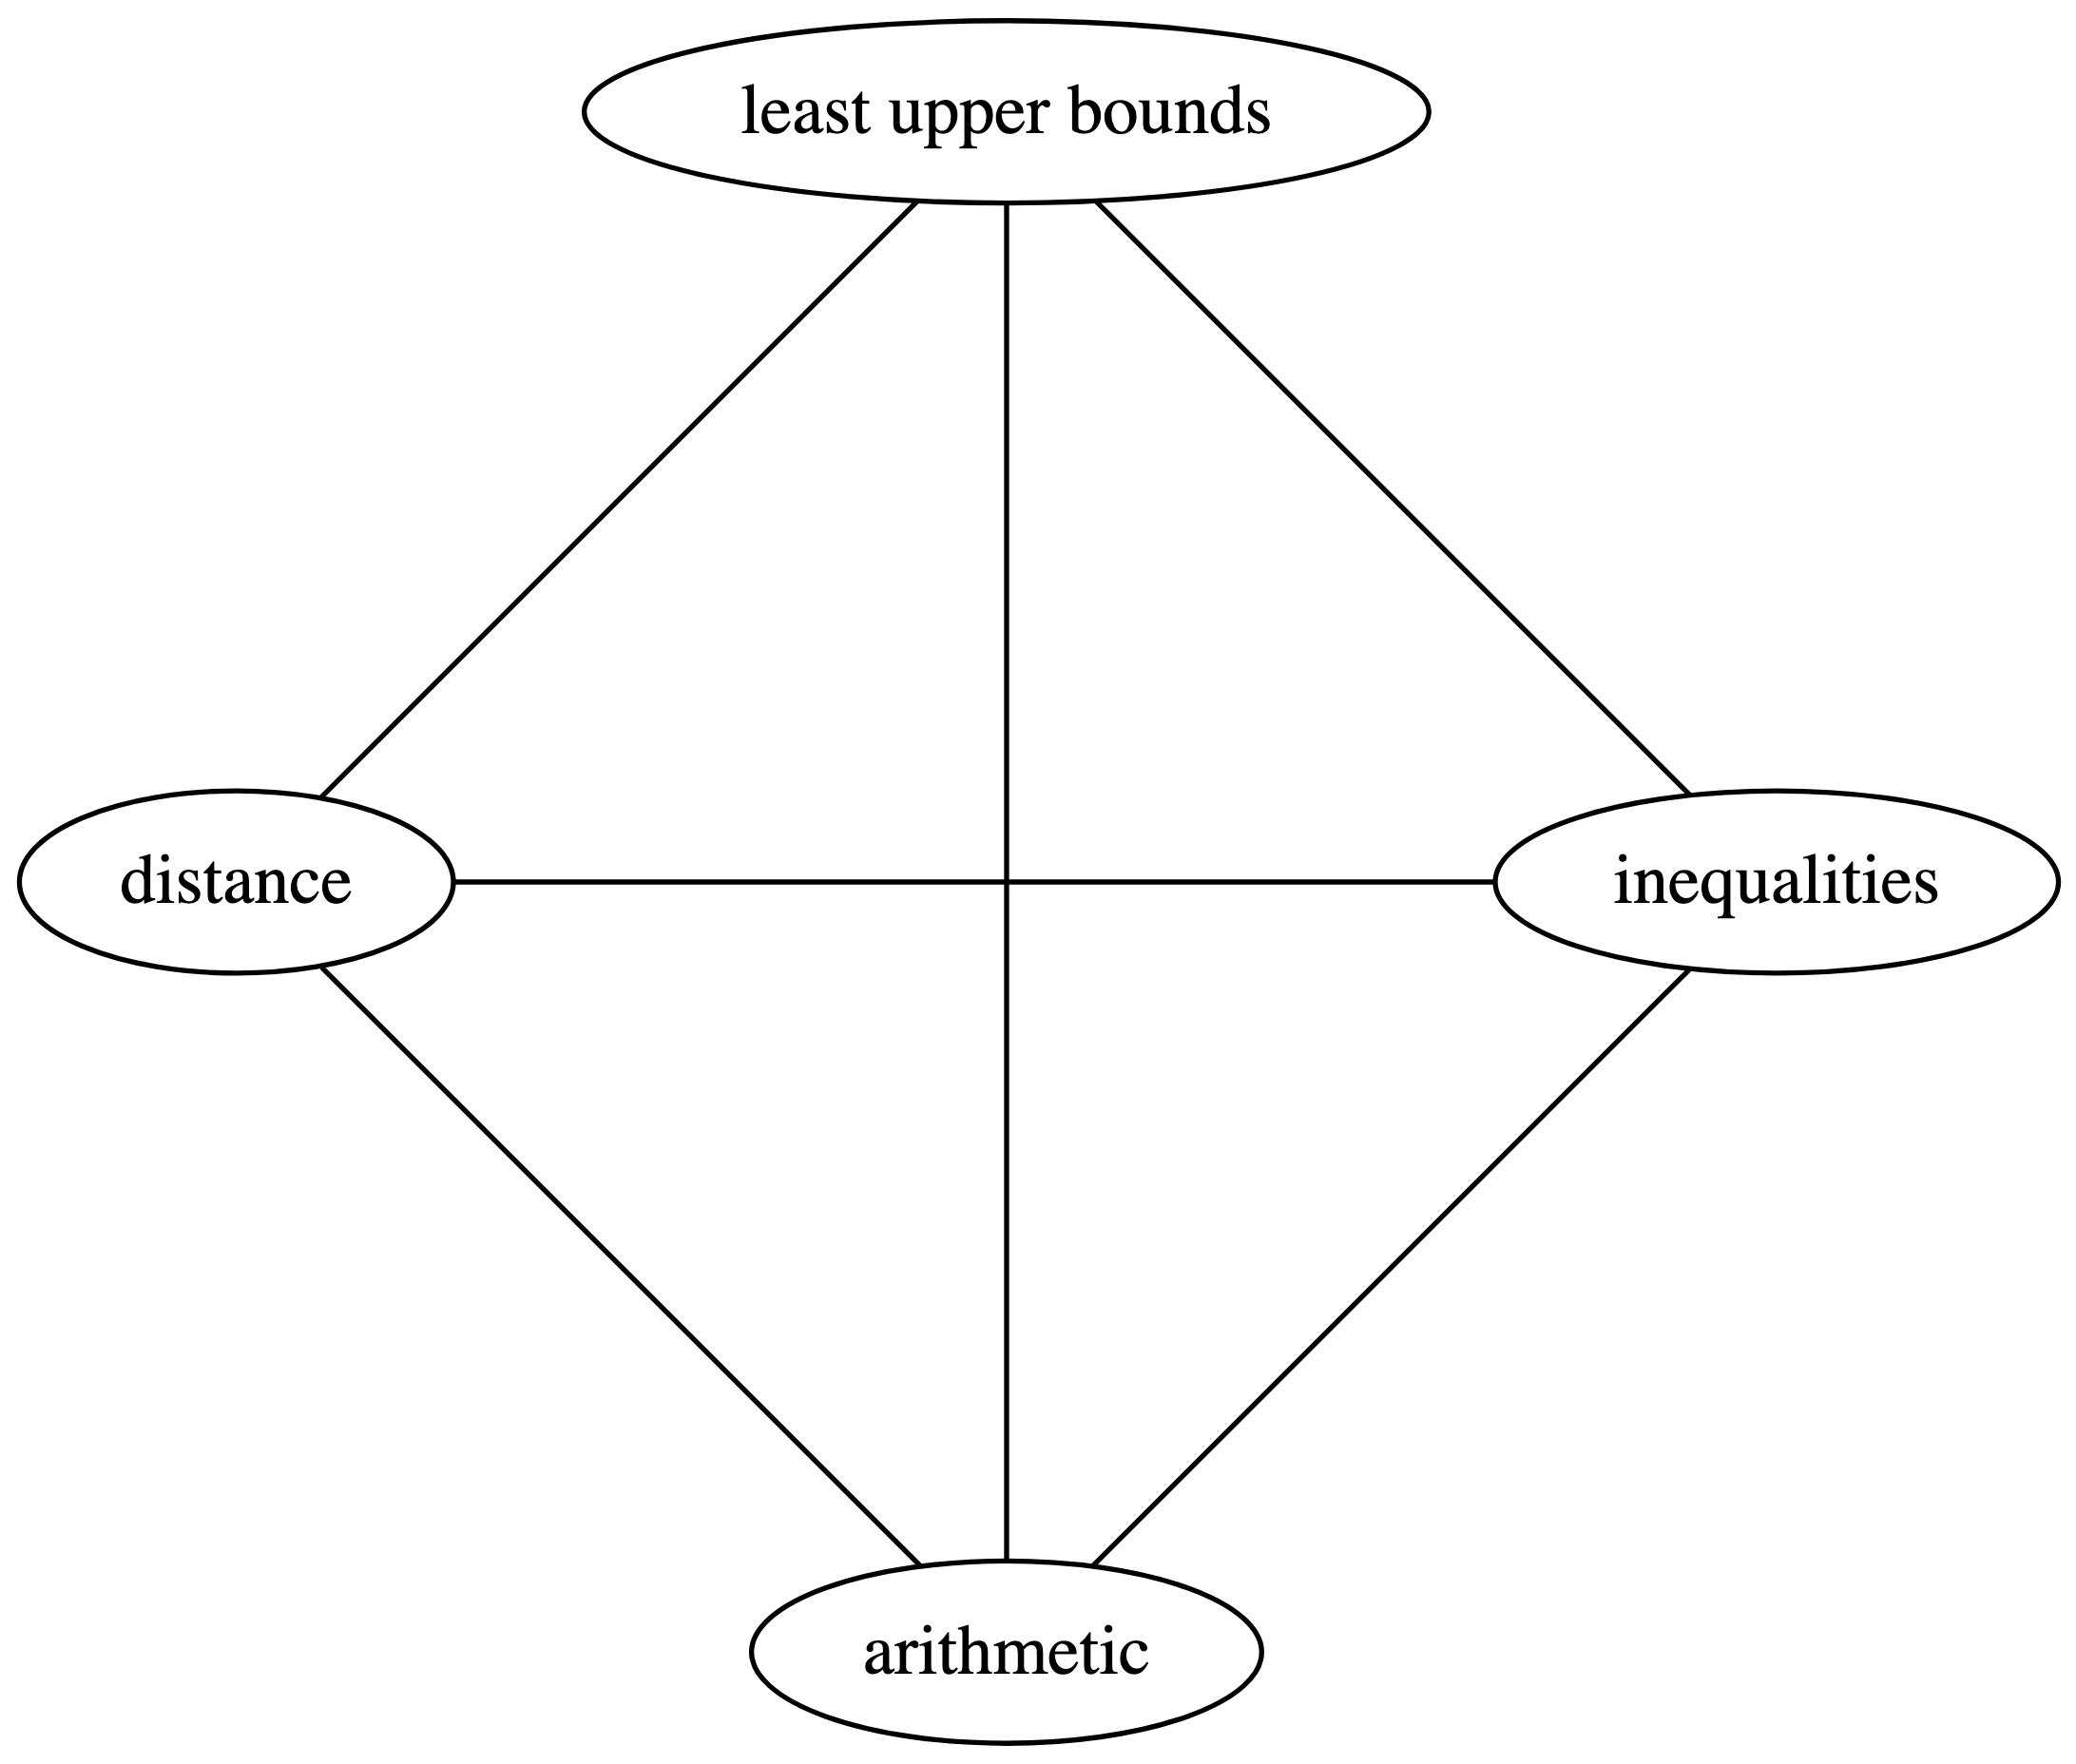
\includegraphics[width=5.5in,height=3.5in]{metric-spaces/r-as-a-metric-space_files/figure-latex/dot-figure-1.png}

\begin{enumerate}
\def\labelenumi{\arabic{enumi}.}
\setcounter{enumi}{1}
\tightlist
\item
  What do we mean when we write \(\max S\)? When are we ``allowed'' to
  use this notation?
\item
  In what sense are the rationals ``all over'' the real number line?
\end{enumerate}

\chapter{Open Sets}\label{open-sets}

\section*{Highlights}\label{highlights-5}
\addcontentsline{toc}{section}{Highlights}

\markright{Highlights}

\begin{itemize}
\tightlist
\item
  Definition of an open ball and open set
\item
  Important equivalent condition to being an open set
\item
  Examples of proving and applying openness
\end{itemize}

\section{Preparation}\label{preparation-5}

An important tool for describing ``closeness'' precisely in calculus is
the open ball.

\begin{definition}[]\protect\hypertarget{def-open-ball}{}\label{def-open-ball}

Suppose \(X\) is a metric space with distance function \(d\). Let
\(a\in X\) and \(r>0\). Then the \textbf{open ball} centered
at\footnote{Sometimes we also say ``around \(a\)''.} \(a\) of radius
\(r\) is defined to be \[\bee_r(a)=\{x\in X\st d(a,x)<r\}.\]

\end{definition}

Other textbooks sometimes call \(\bee_r(a)\) an ``\(r\)-neighborhood''
of \(a\).

\begin{exercise}[]\protect\hypertarget{exr-open-balls-sketch}{}\label{exr-open-balls-sketch}

Describe and draw pictures of open balls in \(\R^3\), \(\R^2\), and
\(\R\).

\end{exercise}

\begin{exercise}[]\protect\hypertarget{exr-open-balls-in-r}{}\label{exr-open-balls-in-r}

Answer the following questions about open balls in \(\R\).

\begin{enumerate}
\def\labelenumi{\arabic{enumi}.}
\tightlist
\item
  Write \(\bee_r(c)\) in interval notation.
\item
  If \(a,b\in\R\) with \(a<b\), is \((a,b)\) an open ball? If so, what
  is its center and radius?
\item
  Is \((0,\infty)\) an open ball? If so, what is its center and radius?
\end{enumerate}

\end{exercise}

The following exercise is meant to prepare you for the definition of an
open set.

\begin{exercise}[]\protect\hypertarget{exr-neighborhood-within-subset-tf}{}\label{exr-neighborhood-within-subset-tf}

Say whether each statement below is true or false and give a brief
justification.

\begin{enumerate}
\def\labelenumi{\arabic{enumi}.}
\tightlist
\item
  ``If \$S=(1,\infty), for each point \(a\in S\) there is an open ball
  centered at \(a\) that lies entirely inside of \(S\).''
\item
  ``If \$S={[}1,\infty), for each point \(a\in S\) there is an open ball
  centered at \(a\) that lies entirely inside of \(S\).''
\end{enumerate}

\end{exercise}

\section{Open Balls}\label{open-balls}

When we apply the definition of an open ball to \(\R\), we realize that
it's an object we've dealt with before; in particular
Theorem~\ref{thm-open-ball-in-r} was really a statement about open balls
on the real number line.

Putting Theorem~\ref{thm-open-ball-in-r} together with the language of
open balls, we now have many equivalent ways of saying the same thing:

{[}TO DO: turn this into a circular diagram with ``In \(\R\)'' in the
center. Then make a smaller one for ``for any metric space''{]}

In \(\R\):
\begin{equation}\phantomsection\label{eq-open-ball-tfae}{ d(a,x)<r \Longleftrightarrow |a-x|<r \Longleftrightarrow x\in(a-r,a+r) \Longleftrightarrow a-r<x<a+r \Longleftrightarrow x\in\bee_r(a)}\end{equation}

The equivalent conditions of (\ref{eq-open-ball-tfae}) in \(\R\) will
show up every day for the rest of the course. The more seamlessly you
can translate among these different ways of saying the same thing, the
easier the course will be.

\begin{quote}
Becoming fluent in (\ref{eq-open-ball-tfae}) is the cheat code for
reading analysis proofs.
\end{quote}

While using the word ``ball'' makes intuitive sense in \(\R^3\) and to a
lesser extent in \(\R^2\), it may feel a little weird in \(\R\); we'll
just need to get used to that. And it gets even stranger when we think
about other metric spaces.

\begin{exercise}[]\protect\hypertarget{exr-open-balls-in-trivial-ms}{}\label{exr-open-balls-in-trivial-ms}

Let \(X\) be a set with the trivial metric (defined in
Exercise~\ref{exr-trivial-metric}). Let \(a\in X\), and describe the
following.

\begin{enumerate}
\def\labelenumi{\arabic{enumi}.}
\tightlist
\item
  \(\bee_2(a)\)
\item
  \(\bee_1(a)\)
\item
  \(\bee_{1/2}(a)\)
\end{enumerate}

\end{exercise}

\begin{exercise}[]\protect\hypertarget{exr-open-balls-in-trivial-ms}{}\label{exr-open-balls-in-trivial-ms}

Consider \(\R^2\) with the ``taxicab metric'' \(d_1\) defined in
Exercise~\ref{exr-taxicab}. Sketch the open ball of radius 2 centered at
the origin.

\end{exercise}

\begin{exercise}[]\protect\hypertarget{exr-open-balls-in-subspace}{}\label{exr-open-balls-in-subspace}

Consider \(X=\{(x,y)\st y\geq0\}\) as a subspace of \(\R^2\). Sketch
\(\bee_2(0,1)\) in the metric space \(S\).

\end{exercise}

An advantage to

\begin{exercise}[]\protect\hypertarget{exr-hausdorff}{}\label{exr-hausdorff}

Suppose \(X\) is a metric space with distance function \(d\). Let
\(a,b\) be distinct points in \(X\). Prove that there exists
\(\epsilon>0\) such that \(\bee_\epsilon(x)\) and \(\bee_\epsilon(y)\)
are disjoint.

\end{exercise}

\section{Open Sets}\label{open-sets-1}

Intuitively we should think of ``open'' sets as ones that do not include
their own boundary

\begin{definition}[]\protect\hypertarget{def-open-set}{}\label{def-open-set}

Let \(X\) be a metric space with distance function \(d\). A subset
\(S\subseteq X\) is called \emph{open} if every point \(a\in S\) has an
open ball around it that lies entirely within \(S\). That is, for all
\(a\in S\), there exists \(r>0\) such that \(\bee_r(a)\subseteq S\).

\end{definition}

\begin{exercise}[]\protect\hypertarget{exr-empty-and-whole-ms-open}{}\label{exr-empty-and-whole-ms-open}

Let \(X\) be a metric space with distance function \(d\). Prove that
\(X\) and \(\varnothing\) are open subsets of \(X\).

\end{exercise}

\begin{exercise}[]\protect\hypertarget{exr-open-balls-are-open}{}\label{exr-open-balls-are-open}

Prove that open balls are open.

\end{exercise}

\begin{exercise}[]\protect\hypertarget{exr-open-negation}{}\label{exr-open-negation}

~

\begin{enumerate}
\def\labelenumi{\arabic{enumi}.}
\tightlist
\item
  Write down what it means for a subset of a metric space to \emph{not}
  be open.
\item
  Write down a careful proof that \((-\infty,2]\) is not an open subset
  of \(\R\).
\end{enumerate}

\end{exercise}

\begin{tcolorbox}[enhanced jigsaw, coltitle=black, left=2mm, bottomrule=.15mm, bottomtitle=1mm, breakable, leftrule=.75mm, opacityback=0, colbacktitle=quarto-callout-caution-color!10!white, toptitle=1mm, opacitybacktitle=0.6, colback=white, colframe=quarto-callout-caution-color-frame, arc=.35mm, title=\textcolor{quarto-callout-caution-color}{\faFire}\hspace{0.5em}{Caution}, titlerule=0mm, rightrule=.15mm, toprule=.15mm]

We are \emph{not} going to call non-open sets ``closed''. The term
``closed'' will have a different definition that we'll get to later.

\end{tcolorbox}

\begin{exercise}[]\protect\hypertarget{exr-complement-of-point-is-open}{}\label{exr-complement-of-point-is-open}

Suppose \(X\) is a metric space and let \(a\in X\). Prove that
\(\{a\}^\cee\) is open.

\end{exercise}

\section*{Review Questions}\label{review-questions-5}
\addcontentsline{toc}{section}{Review Questions}

\markright{Review Questions}

\begin{enumerate}
\def\labelenumi{\arabic{enumi}.}
\tightlist
\item
  What is the definition of an open ball in a metric space?
\item
  What is the definition of an open set? Can you draw a picture
  representing this definition?
\item
  What are the open balls in \(\R\)?
\end{enumerate}

\chapter{Properties of Open Sets}\label{properties-of-open-sets}

\section*{Highlights}\label{highlights-6}
\addcontentsline{toc}{section}{Highlights}

\markright{Highlights}

\begin{itemize}
\tightlist
\item
  Characterization of open sets as unions of open balls
\item
  Unions and intersections of open sets
\end{itemize}

\section{Preparation}\label{preparation-6}

\begin{theorem}[]\protect\hypertarget{thm-open-set-tfae}{}\label{thm-open-set-tfae}

Let \(X\) be a metric space and \(U\subseteq X\). The following are
equivalent.

\begin{enumerate}
\def\labelenumi{\arabic{enumi}.}
\tightlist
\item
  \(U\) is open.
\item
  \(U\) is a union of open balls.
\end{enumerate}

\end{theorem}

\begin{exercise}[]\protect\hypertarget{exr-prove-open-set-tfae}{}\label{exr-prove-open-set-tfae}

Prove Theorem~\ref{thm-open-set-tfae}

\end{exercise}

Theorem~\ref{thm-open-set-tfae} is another ``the following are
equivalent'' theorem. We love these because anytime there is a proof
involving an open set, we get to pick which condition to use.

\begin{theorem}[]\protect\hypertarget{thm-unions-and-intersections-of-open-sets}{}\label{thm-unions-and-intersections-of-open-sets}

~

\begin{enumerate}
\def\labelenumi{\arabic{enumi}.}
\tightlist
\item
  The union of any collection of open sets is open.
\item
  The intersection of any finite collection of open sets is open.
\end{enumerate}

\end{theorem}

\begin{exercise}[]\protect\hypertarget{exr-unions-of-open-sets}{}\label{exr-unions-of-open-sets}

Prove Part 1 of Theorem~\ref{thm-unions-and-intersections-of-open-sets}.

Hint: Will it be easier to work with the \emph{definition} of openness,
or Condition 2 of Theorem~\ref{thm-open-set-tfae} for this proof?

\end{exercise}

\begin{proof}[Setup of proof of Part 2 of
Theorem~\ref{thm-unions-and-intersections-of-open-sets}]
Suppose \(U_1,\ldots,U_n\) are open and let \(U=\bigcap_{i=1}^n U_i\).
We will prove \(U\) is open using the definition of openness, so we
start by supposing that \(x\in U\). This means \(x\in U_i\) for all
\(i=1,\ldots,n\). Therefore, applying the definition of openness to each
\(U_i\), there exists \(r_i\) such that
\(\bee_{r_i}(x)\subseteq U_i\subseteq U\).
\end{proof}

\begin{exercise}[]\protect\hypertarget{exr-intersections-of-open-sets}{}\label{exr-intersections-of-open-sets}

Finish the proof of Part 2 of
Theorem~\ref{thm-unions-and-intersections-of-open-sets}.

\end{exercise}

\begin{exercise}[]\protect\hypertarget{exr-infinite-intersection-of-open-sets}{}\label{exr-infinite-intersection-of-open-sets}

~

\begin{enumerate}
\def\labelenumi{\arabic{enumi}.}
\tightlist
\item
  At what point in the proof of Part 2 of
  Theorem~\ref{thm-unions-and-intersections-of-open-sets} did you use
  the fact that we were only dealing with \emph{finitely many} open
  sets?
\item
  Give an example of a(n infinite) collection of open sets whose
  intersection is \emph{not} open. (Remember, \(\varnothing\) is open!)
\end{enumerate}

\end{exercise}

{[}Two images? Desmos interactives?{]}

\section*{Review Questions}\label{review-questions-6}
\addcontentsline{toc}{section}{Review Questions}

\markright{Review Questions}

\section{To include}\label{to-include}

\begin{enumerate}
\def\labelenumi{\arabic{enumi}.}
\setcounter{enumi}{4}
\tightlist
\item
  Desmos app with C\&C Fig 3.1 and fading-in/out open balls
\item
  Visual proof that the open square is open (and that the closed square
  is not)
\item
  Negate ``open''
\end{enumerate}

\chapter{Boundedness}\label{boundedness}

\section*{Highlights}\label{highlights-7}
\addcontentsline{toc}{section}{Highlights}

\markright{Highlights}

\begin{itemize}
\tightlist
\item
  Definition of a bounded subset of a metric space
\item
  Equivalent conditions to boundedness
\item
  Boundedness in \(\R\) is equivalent to ``bounded above and below''
\end{itemize}

\section{Preparation}\label{preparation-7}

\begin{theorem}[]\protect\hypertarget{thm-bounded}{}\label{thm-bounded}

Let \(X\) be a metric space and let \(S\subseteq X\). Then the following
are equivalent.

\begin{enumerate}
\def\labelenumi{\arabic{enumi}.}
\tightlist
\item
  For any \(a\in X\), there exists \(r>0\) such that
  \(S\subseteq B_r(a)\).
\item
  There exists \(a\in X\) and \(r>0\) such that \(S\subseteq B_r(a).\)
\end{enumerate}

In this case, we say \(S\) is \textbf{bounded}.

\end{theorem}

You will prove Theorem~\ref{thm-bounded} in
Exercise~\ref{exr-bounded-tfae-proof} below.

\begin{tcolorbox}[enhanced jigsaw, coltitle=black, left=2mm, bottomrule=.15mm, bottomtitle=1mm, breakable, leftrule=.75mm, opacityback=0, colbacktitle=quarto-callout-note-color!10!white, toptitle=1mm, opacitybacktitle=0.6, colback=white, colframe=quarto-callout-note-color-frame, arc=.35mm, title=\textcolor{quarto-callout-note-color}{\faInfo}\hspace{0.5em}{Note}, titlerule=0mm, rightrule=.15mm, toprule=.15mm]

Theorem~\ref{thm-bounded} is both a theorem and a definition. Once we
prove the conditions are equivalent, we can refer to any one of them as
``the'' definition of bounded.

\end{tcolorbox}

\begin{exercise}[]\protect\hypertarget{exr-boundedness-tfae-reflection}{}\label{exr-boundedness-tfae-reflection}

~

\begin{enumerate}
\def\labelenumi{\arabic{enumi}.}
\tightlist
\item
  If a problem asks you to \emph{prove} that a set is bounded, which of
  the two conditions from Theorem~\ref{thm-bounded} would you choose to
  work with, and why?
\item
  If a problem tells you to assume that a set is bounded and you need to
  \emph{apply} boundedness in order to prove something else, which of
  the two conditions from Theorem~\ref{thm-bounded} would you choose to
  work with, and why?
\end{enumerate}

\end{exercise}

\begin{exercise}[]\protect\hypertarget{exr-unbounded}{}\label{exr-unbounded}

Negate each of the two equivalent characterizations of boundedness.

\end{exercise}

A subset of a metric space that is not bounded is called
\textbf{unbounded}.

\section{Properties of Boundedness}\label{properties-of-boundedness}

We start with proving that the two definitions of boundedness are in
fact equivalent.

\begin{exercise}[]\protect\hypertarget{exr-bounded-tfae-proof}{}\label{exr-bounded-tfae-proof}

Prove Theorem~\ref{thm-bounded}.

\end{exercise}

\begin{tcolorbox}[enhanced jigsaw, coltitle=black, left=2mm, bottomrule=.15mm, bottomtitle=1mm, breakable, leftrule=.75mm, opacityback=0, colbacktitle=quarto-callout-tip-color!10!white, toptitle=1mm, opacitybacktitle=0.6, colback=white, colframe=quarto-callout-tip-color-frame, arc=.35mm, title=\textcolor{quarto-callout-tip-color}{\faLightbulb}\hspace{0.5em}{Hint}, titlerule=0mm, rightrule=.15mm, toprule=.15mm]

\begin{enumerate}
\def\labelenumi{\arabic{enumi}.}
\tightlist
\item
  One of the two implications should be very quick to prove!
\item
  Note that \(a\) might lie outside of \(S\) for either of the two
  conditions.
\end{enumerate}

\end{tcolorbox}

\begin{exercise}[]\protect\hypertarget{exr-unbounded-subset-of-r2}{}\label{exr-unbounded-subset-of-r2}

Let \(S=\{(n,n)\in\R^2\st n\in\N\}\). Draw a picture of \(S\) and give a
careful proof that \(S\) is unbounded.

\end{exercise}

\begin{exercise}[]\protect\hypertarget{exr-union-of-two-bounded-is-bounded}{}\label{exr-union-of-two-bounded-is-bounded}

Suppose \(S_1\) and \(S_2\) are bounded subsets of a metric space \(X\).
Prove that \(S_1\cup S_2\) is bounded.

\end{exercise}

\section{\texorpdfstring{Boundedness in
\(\R\)}{Boundedness in \textbackslash R}}\label{boundedness-in-r}

As ever, what we really care about is how this concept applies to \(\R\)
and how the concepts defined thus far interact. We've already defined
``bounded above'' and ``bounded below''. The next theorem will connect
these definitions to our new more general defintion of ``bounded'' for
metric spaces.

\begin{theorem}[]\protect\hypertarget{thm-boundedness-in-r}{}\label{thm-boundedness-in-r}

Suppose \(S\subseteq\R\).Then the following are equivalent.

\begin{enumerate}
\def\labelenumi{\arabic{enumi}.}
\tightlist
\item
  \(S\) is bounded.
\item
  \(S\) has an upper bound and a lower bound.
\item
  There exists \(K>0\) such that for all \(x\in X\), \(|x|<K\).
\end{enumerate}

\end{theorem}

\begin{exercise}[]\protect\hypertarget{exr-boundedness-in-r}{}\label{exr-boundedness-in-r}

Prove Theorem~\ref{thm-boundedness-in-r}.

\end{exercise}

\begin{exercise}[]\protect\hypertarget{exr-unbounded-subset-of-r}{}\label{exr-unbounded-subset-of-r}

Prove that the complement of an unbounded subset of \(\R\) is bounded.

\end{exercise}

\section*{Review Questions}\label{review-questions-7}
\addcontentsline{toc}{section}{Review Questions}

\markright{Review Questions}

\begin{enumerate}
\def\labelenumi{\arabic{enumi}.}
\tightlist
\item
  What does it mean for a subset of a metric space to be bounded?
  Unbounded?
\item
  With Theorem~\ref{thm-bounded} and Theorem~\ref{thm-boundedness-in-r},
  we have four equivalent ways of describing boundedness in \(\R\); what
  are they?
\end{enumerate}

\part{Sequences}

\chapter{Talking About Sequences}\label{sec-sequences}

\section*{Highlights}\label{highlights-8}
\addcontentsline{toc}{section}{Highlights}

\markright{Highlights}

\begin{itemize}
\tightlist
\item
  Definition of a sequence as a function with domain \(\N\)
\item
  Sequence notation and vocabulary
\item
  Properties that a sequence may or may not have
\end{itemize}

\section{Preparation}\label{preparation-8}

Sequences are one of the fundamental objects of study in real analysis.
They form the theoretical basis for blah blah blah.

\begin{definition}[]\protect\hypertarget{def-sequence}{}\label{def-sequence}

A \textbf{sequence} in \(X\) is a function \(s:\N\rightarrow X\).

\end{definition}

In this context, instead of using standard function notation
\(s(1),s(2),\ldots,s(n),\ldots\), we instead use subscripts and write
\(s_1,s_2,\ldots,s_n,\ldots\). We refer to a particular \(s_n\) as a
\textbf{term} of the sequence and to the input/subscript \(n\) as its
\textbf{index} or \textbf{position} in the sequence.

\begin{tcolorbox}[enhanced jigsaw, coltitle=black, left=2mm, bottomrule=.15mm, bottomtitle=1mm, breakable, leftrule=.75mm, opacityback=0, colbacktitle=quarto-callout-caution-color!10!white, toptitle=1mm, opacitybacktitle=0.6, colback=white, colframe=quarto-callout-caution-color-frame, arc=.35mm, title=\textcolor{quarto-callout-caution-color}{\faFire}\hspace{0.5em}{Caution}, titlerule=0mm, rightrule=.15mm, toprule=.15mm]

Under this definition, by ``sequence'' we always mean ``infinite
sequence'' since the domain is \(\N\).

\end{tcolorbox}

\begin{tcolorbox}[enhanced jigsaw, coltitle=black, left=2mm, bottomrule=.15mm, bottomtitle=1mm, breakable, leftrule=.75mm, opacityback=0, colbacktitle=quarto-callout-note-color!10!white, toptitle=1mm, opacitybacktitle=0.6, colback=white, colframe=quarto-callout-note-color-frame, arc=.35mm, title=\textcolor{quarto-callout-note-color}{\faInfo}\hspace{0.5em}{Note}, titlerule=0mm, rightrule=.15mm, toprule=.15mm]

For now, as we get comfortable with the idea of a sequence, we will
insist that our sequences start at \(s_1\). Later on, especially when
dealing with infinite sums (known as series), we will relax this
constraint since it is often convenient to start at \(0\) or some other
integer.

\end{tcolorbox}

The \textbf{range} of \((a_n)\) is \(\{a_n\st n\in\N\}\).

\begin{exercise}[]\protect\hypertarget{exr-finite-range}{}\label{exr-finite-range}

Can a sequence have a range that is finite? Explain.

\end{exercise}

\section{Sequence Properties}\label{sequence-properties}

Below are several properties of sequences that we will need moving
forward.

\begin{definition}[]\protect\hypertarget{def-sequence-props-any-codomain}{}\label{def-sequence-props-any-codomain}

Let \((a_n)\) be a sequence in a metric space. Then \((a_n)\) is said
to\(\ldots\)

\begin{enumerate}
\def\labelenumi{\arabic{enumi}.}
\tightlist
\item
  be \textbf{constant} if \(a_i=a_j\) for all \(i,j\in\N\).
\item
  have \textbf{distinct terms} if \(a_i\neq a_j\) whenever \(i\neq j\).
\item
  be \textbf{bounded} if its range is.
\end{enumerate}

\end{definition}

For sequences in \(\R\), we can make some further definitions.

\begin{definition}[]\protect\hypertarget{def-sequence-props-any-codomain}{}\label{def-sequence-props-any-codomain}

Let \((a_n)\) be a sequence in \(\R\). Then \((a_n)\) is said to
be\(\ldots\)

\begin{enumerate}
\def\labelenumi{\arabic{enumi}.}
\tightlist
\item
  \textbf{increasing} if \(i\leq j\) implies \(a_i\leq a_j\).
\item
  \textbf{decreasing} if \(i\leq j\) implies \(a_i\geq a_j\).
\item
  \textbf{strictly increasing} (repsectively \textbf{strictly
  decreasing}) if \(i< j\) implies \(a_i< a_j\) (respectively
  \(a_i>a_j\)).
\item
  \textbf{monotonic} if it is either only increasing or only decreasing,
  and \textbf{strictly monotonic} if it is either only strictly
  increasing or only strictly decreasing.
\item
  \textbf{bounded above} (respectively, \textbf{bounded below}) if its
  range is.
\end{enumerate}

\end{definition}

\begin{exercise}[]\protect\hypertarget{exr-sequence-prop-example-generation}{}\label{exr-sequence-prop-example-generation}

Give an example of a sequence in \(\R\) with the properties below, or
prove that no such example exists.

\begin{enumerate}
\def\labelenumi{\arabic{enumi}.}
\tightlist
\item
  A sequence which is both increasing and decreasing.
\item
  A sequence which is strictly increasing and bounded above.
\item
  A bounded sequence of distinct terms.
\item
  A sequence of distinct terms that is increasing but not strictly
  increasing.
\item
  An unbounded sequence which is not monotonic.
\item
  A sequence with a finite range that is unbounded.
\end{enumerate}

\end{exercise}

\begin{theorem}[The Amazingly Useful
Theorem]\protect\hypertarget{thm-amazingly-useful}{}\label{thm-amazingly-useful}

Suppose \((i_n)\) is a strictly increasing sequence in \(\N\). Then
\(i_n\geq n\).

\end{theorem}

\begin{exercise}[]\protect\hypertarget{exr-amazingly-useful-proof}{}\label{exr-amazingly-useful-proof}

Prove Theorem~\ref{thm-amazingly-useful} by induction.

\end{exercise}

\section{Visualizing Sequences}\label{visualizing-sequences}

We often visualize a sequence \((a_n)\) by showing either its
\emph{range} in the codomain or, for sequences in \(\R\), its
\emph{graph} in the cartesian plane.

\begin{figure}

\begin{minipage}{\linewidth}

\centering{

\pandocbounded{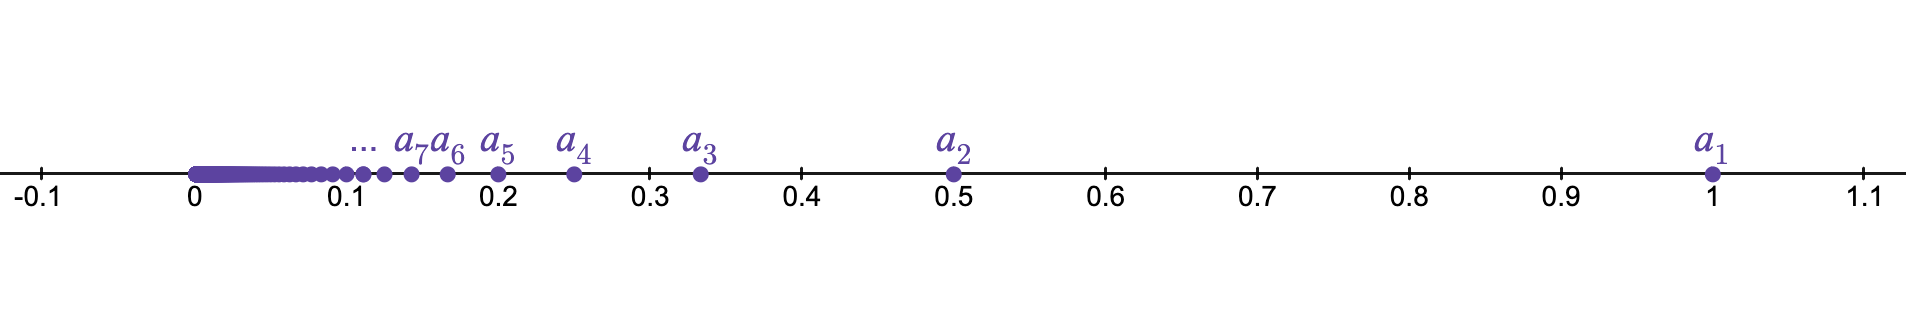
\includegraphics[keepaspectratio]{sequences/recip-seq-range.png}}

}

\subcaption{\label{fig-recip-seq-range}The sequence
\(\left(\frac{1}{n}\right)\) in \(\R\).}

\end{minipage}%
\newline
\begin{minipage}{\linewidth}

\centering{

\pandocbounded{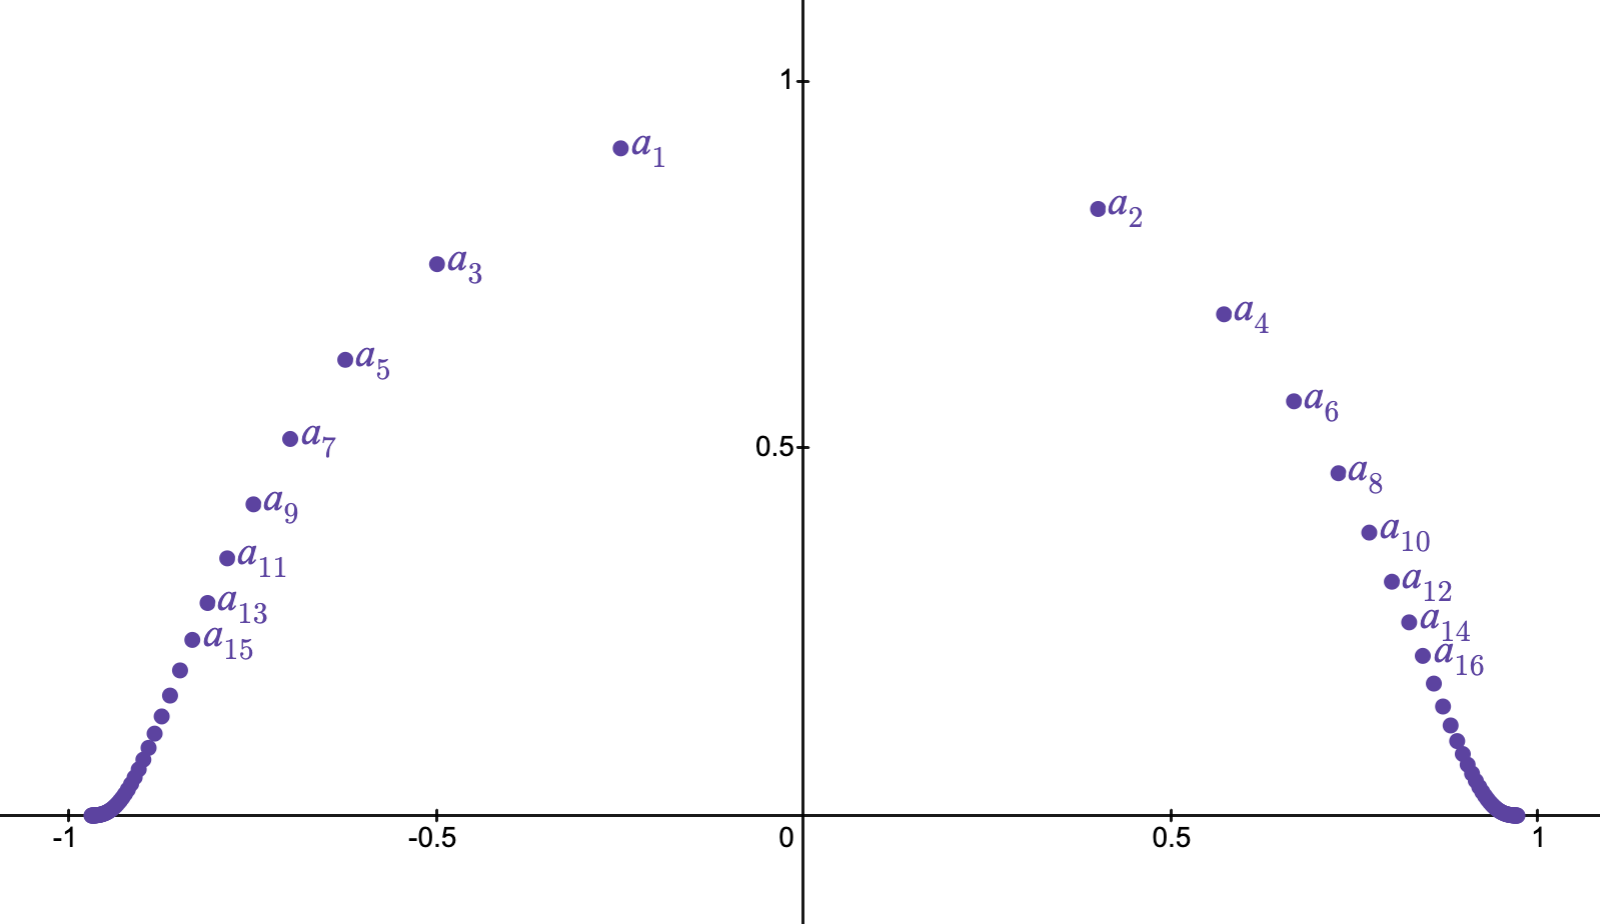
\includegraphics[keepaspectratio]{sequences/seq-range-r2.png}}

}

\subcaption{\label{fig-seq-range-r2}A sequence in \(\R^2\)}

\end{minipage}%

\caption{\label{fig-sequence-ranges}Here we show the ranges of two
sequences. When plotting the range of a sequence, we usually number at
least the first several terms.}

\end{figure}%

When plotting the graph of a sequence, we use the horizontal axis for
the indices (in \(\N\)) and the vertical axis for the terms (in \(\R\)).

\begin{figure}

\begin{minipage}{\linewidth}

\centering{

\pandocbounded{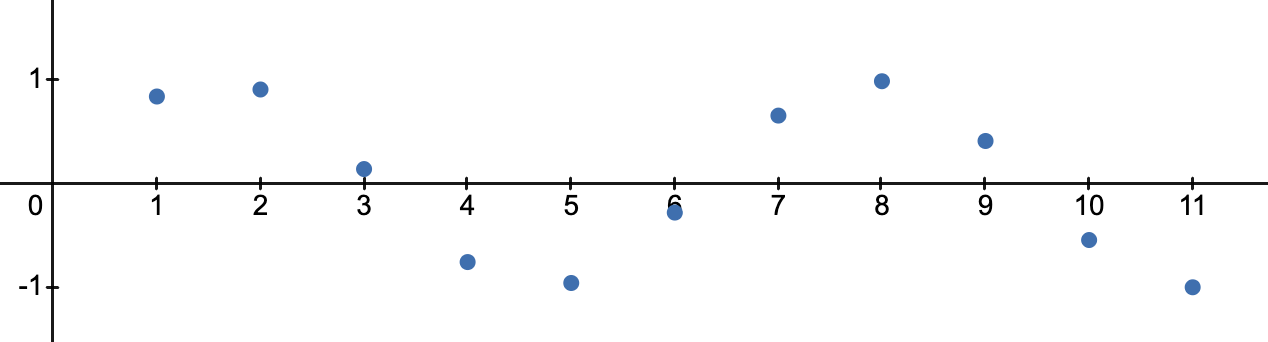
\includegraphics[keepaspectratio]{sequences/sin-n-graph.png}}

}

\subcaption{\label{fig-sin-n-graph}The sequence \((\sin(n))\).}

\end{minipage}%
\newline
\begin{minipage}{\linewidth}

\centering{

\pandocbounded{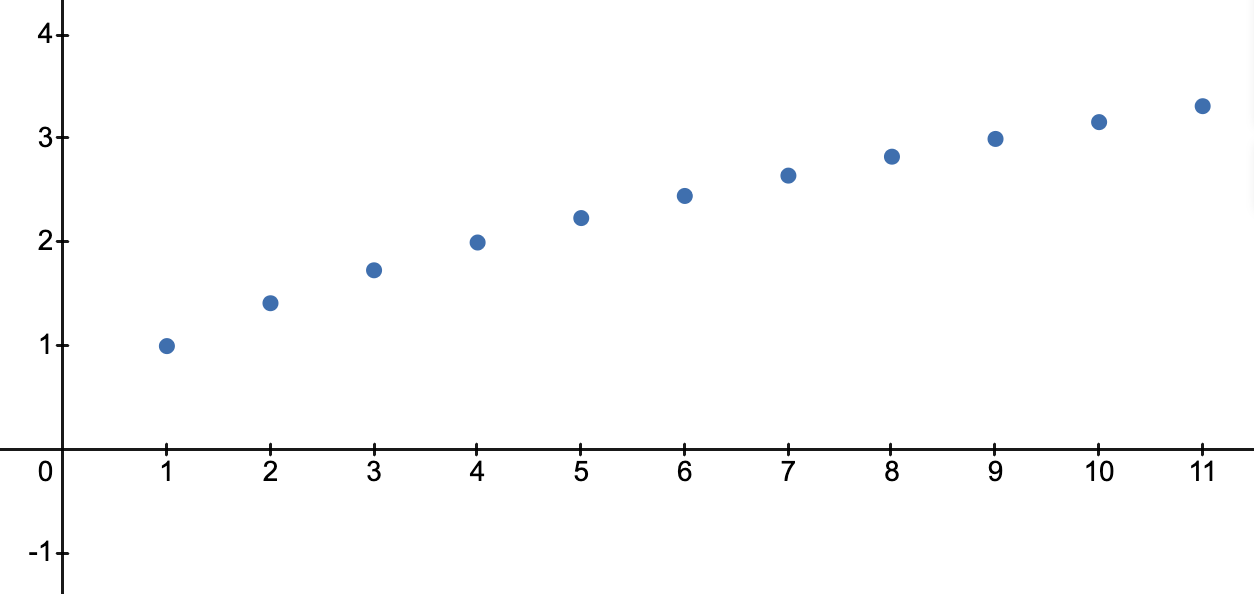
\includegraphics[keepaspectratio]{sequences/sqrt-n-graph.png}}

}

\subcaption{\label{fig-sqrt-n-graph}The sequence \((\sqrt n)\).}

\end{minipage}%
\newline
\begin{minipage}{\linewidth}

\centering{

\pandocbounded{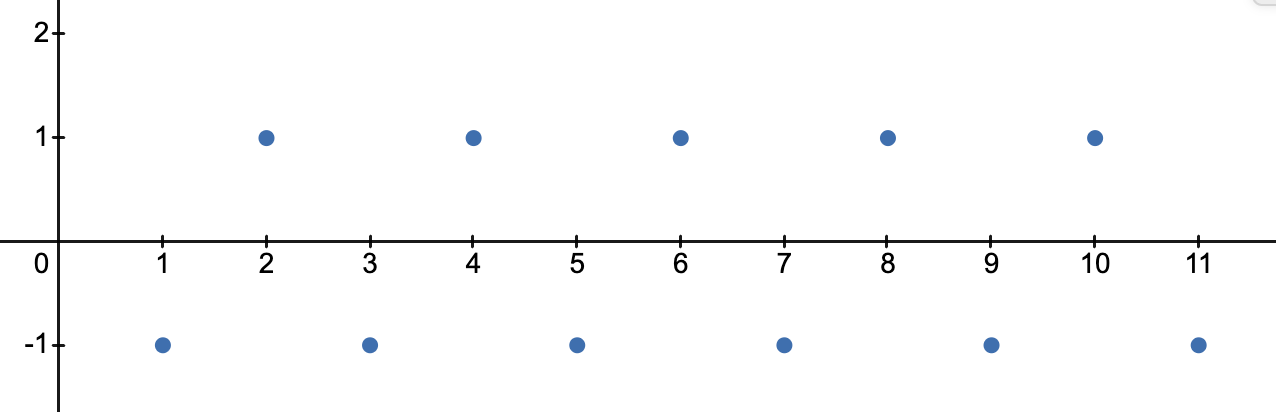
\includegraphics[keepaspectratio]{sequences/alternating-graph.png}}

}

\subcaption{\label{fig-alternating-graph}The sequence \(((-1)^n)\).}

\end{minipage}%

\caption{\label{fig-sequence-graph}The graphs of three sequences in
\(\R\).}

\end{figure}%

\begin{tcolorbox}[enhanced jigsaw, coltitle=black, left=2mm, bottomrule=.15mm, bottomtitle=1mm, breakable, leftrule=.75mm, opacityback=0, colbacktitle=quarto-callout-tip-color!10!white, toptitle=1mm, opacitybacktitle=0.6, colback=white, colframe=quarto-callout-tip-color-frame, arc=.35mm, title=\textcolor{quarto-callout-tip-color}{\faLightbulb}\hspace{0.5em}{Hint}, titlerule=0mm, rightrule=.15mm, toprule=.15mm]

A collapsed hint.

\end{tcolorbox}

\section*{Review Questions}\label{review-questions-8}
\addcontentsline{toc}{section}{Review Questions}

\markright{Review Questions}

\begin{enumerate}
\def\labelenumi{\arabic{enumi}.}
\tightlist
\item
  Question 1
\item
  Question 2
\end{enumerate}

\section{To include}\label{to-include-1}

\begin{itemize}
\tightlist
\item
  Quick teaser about convergence
\item
  Lots of examples of sequences
\item
  Constructing sequences by induction?
\end{itemize}

\chapter{Subsequences}\label{subsequences}

\section*{Highlights}\label{highlights-9}
\addcontentsline{toc}{section}{Highlights}

\markright{Highlights}

\begin{itemize}
\tightlist
\item
  highlight 1
\item
  highlight 2
\end{itemize}

\section{Preparation}\label{preparation-9}

(Pre-class reading and exercises)

\section{Body}\label{body}

What will be covered in class plus exercises

\begin{tcolorbox}[enhanced jigsaw, coltitle=black, left=2mm, bottomrule=.15mm, bottomtitle=1mm, breakable, leftrule=.75mm, opacityback=0, colbacktitle=quarto-callout-tip-color!10!white, toptitle=1mm, opacitybacktitle=0.6, colback=white, colframe=quarto-callout-tip-color-frame, arc=.35mm, title=\textcolor{quarto-callout-tip-color}{\faLightbulb}\hspace{0.5em}{Hint}, titlerule=0mm, rightrule=.15mm, toprule=.15mm]

A collapsed hint.

\end{tcolorbox}

\section{More sections}\label{more-sections}

More content

\section*{Review Questions}\label{review-questions-9}
\addcontentsline{toc}{section}{Review Questions}

\markright{Review Questions}

\begin{enumerate}
\def\labelenumi{\arabic{enumi}.}
\tightlist
\item
  Question 1
\item
  Question 2
\end{enumerate}

\section{To include}\label{to-include-2}

\begin{itemize}
\tightlist
\item
  Subsequence index theorem
\item
  ``Nth tail'' and ``eventually''
\item
  Exercises of the form ``which properties pass to subsequences?''
\item
  Examples of proofs that are made easier by considering subsequences
\end{itemize}

\chapter{Series Basics}\label{series-basics}

In this section, we build on what we learned about sequences to talk
about one of their most important use cases: series. Loosely speaking,
we think of a series as an ``infinite sum'', and one of the primary
questions we seek to address is when a series converges to a finite
number and when it doesn't. Consider for example, the four infinite sums
below:

\begin{equation}\phantomsection\label{eq-first-examples}{\begin{array}{l}
1+2+3+4+\cdots \\~\\
1+(-1)+1+(-1)+\cdots \\~\\
1+\frac{1}{2}+\frac{1}{3}+\frac{1}{4}+\cdots \\~\\
%1+\left(-\frac{1}{2}\right)+\frac{1}{4}+\left(-\frac{1}{8}\right)+\cdots
1+\frac{1}{2}+\frac{1}{4}+\frac{1}{8}+\frac{1}{16}+\cdots
\end{array}}\end{equation}

Some of these might strike you as obviously undefined or obviously
convergent, but others may not. In what follows below, we'll make a
precise definition of what we mean by convergent so that we can prove
theorems and talk coherently about examples.\footnote{There are actually
  several theories of convergent series which are useful in different
  contexts. We'll present the most standard version here.}

\section{Series and Partial Sums}\label{series-and-partial-sums}

Suppose \((a_n)\) is a sequence in \(\mathbb{R}\). Then the
\emph{series} with terms \((a_n)\) is the formal expression

\[\sum_{i=1}^\infty a_i=a_1+a_2+\cdots\]

By ``formal expression'' I mean that we are not considering this
expression to represent a number; it's just notation meant to express
the \emph{idea} of an infinite sum. Sometimes we abbreviate the notation
as \(\sum a_i\).

\begin{definition}[Partial
Sums]\protect\hypertarget{def-partial-sum}{}\label{def-partial-sum}

The \emph{sequence of partial sums} of the series
\(\displaystyle\sum_{i=1}^\infty a_i\) is the sequence \((s_n)\) defined
by \[ s_n=\sum_{i=1}^n a_i = a_1+\cdots+a_n \]

\end{definition}

This means that \[\begin{array}{ccl}
s_1&=&a_1\\
s_2&=&a_1+a_2\\
s_3&=&a_1+a+2+a_3\\
&\vdots&
\end{array}\]

We now define convergence of series in terms of the partial sums.

\begin{definition}[Series
Convergence]\protect\hypertarget{def-series-convergence}{}\label{def-series-convergence}

The series \(\displaystyle\sum_{i=1}^\infty a_i\) is said to
\emph{converge} or \emph{diverge} when its sequence of partial sums
\((s_n)\) does. If \(s_n\rightarrow S\), we call \(S\) the \emph{sum} of
the series.

\end{definition}

In the case that \(\displaystyle\sum_{i=1}^\infty a_i\) has sum \(S\),
we sometimes abuse notation slightly and use the expression
\(\displaystyle\sum_{i=1}^\infty a_i\) to represent the number \(S\).

As an example of the vocabulary in the action, the series
\(\displaystyle \sum_{i=1}^\infty \frac{2}{3^i}\)

\begin{itemize}
\tightlist
\item
  has \emph{terms} given by the sequence \(\left(\frac{2}{3^i}\right)\)
  or \(\frac{2}{3},\frac{2}{9},\frac{2}{27},\frac{2}{81},\cdots\)
\item
  has \emph{partial sums}
  \(\frac{2}{3},\frac{2}{3}+\frac{2}{9},\frac{2}{3}+\frac{2}{9}+\frac{2}{27},\ldots\).
  These simplifies to \(\frac{2}{3},\frac{8}{9},\frac{26}{27},\ldots\)
  or \(\left(\frac{3^i-1}{3^i}\right)\).
\item
  \emph{converges} with a \emph{sum} of \(1\).
\end{itemize}

\begin{exercise}[]\protect\hypertarget{exr-partial-sum-practice}{}\label{exr-partial-sum-practice}

Write each of the four infinite sums in Equation~\ref{eq-first-examples}
using series notation. Then write out the first 6 partial sums for each.
Are there any you can tell right away converge or diverge?

\end{exercise}

\section{Working with Partial Sums}\label{working-with-partial-sums}

We start with an important class of series called \emph{geometric
series}.

\begin{example}[Geometric
Series]\protect\hypertarget{exm-geometric}{}\label{exm-geometric}

For \(a\neq 0\) and any \(r\in\mathbb{R}\), a series of the form
\[\sum_{i=0}^\infty ar^n\] is called a \emph{geometric series}. This
series converges to \(\frac{a}{1-r}\) when \(|r|<1\) and diverges
otherwise.

\end{example}

\begin{proof}
To determine whether the series converges, we analyze its partial sums
in cases.

If \(|r|\neq1\), we can use some algebraic tricks to simplify the
expression for the partial sum \(s_n\): \[\begin{array}{rcl}
  s_n&=&a+ar+ar^2+cdots+ar^n\\
  &=&a(1+r+r^2+\cdots+r^n)\\
  &=&\displaystyle\frac{a(1-r^{n+1})}{1-r}
\end{array}\] If \(|r|<1\), then \(r^{n+1}\rightarrow0\), so using what
we know about sequences and arithmetic, we can say
\(s_n\rightarrow\frac{a}{1-r}\).

If \(|r|>1\), then \((r^{n+1})\) diverges. So if, by way of
contradiction, we assume the partial sums \((s_n)\) did converge to some
value \(S\), then we could say that the sequence
\(\left(1-s_n\frac{1-r}{a}\right)\) converges to \(1-L\frac{1-r}{a}\).
However \(1-s_n\frac{1-r}{a}=r^{n+1}\), which we already said
diverges.\footnote{I am bending over backwards here to make precise the
  intuition that ``Since \((r^{n+1})\) diverges, so must an sequence
  involving it''. Unfortunately, that reasoning doesn't always
  work--think about \((\sqrt{n+1} - \sqrt{n})\) which converges despite
  being the sum of two divergent sequences--so a proof of the style
  shown here is appropriate.}

We leave the cases where \(r=\pm1\) to the reader in
Exercise~\ref{exr-geometric-with-r-pm1} below.
\end{proof}

\begin{exercise}[]\protect\hypertarget{exr-geometric-with-r-pm1}{}\label{exr-geometric-with-r-pm1}

Finish the proof of Example~\ref{exm-geometric} by proving that the
geometric series diverges when \(r=1\) and when \(r=-1\). (Hint: what
are the partial sums in each of these cases?)

\end{exercise}

\begin{tcolorbox}[enhanced jigsaw, coltitle=black, left=2mm, bottomrule=.15mm, bottomtitle=1mm, breakable, leftrule=.75mm, opacityback=0, colbacktitle=quarto-callout-note-color!10!white, toptitle=1mm, opacitybacktitle=0.6, colback=white, colframe=quarto-callout-note-color-frame, arc=.35mm, title=\textcolor{quarto-callout-note-color}{\faInfo}\hspace{0.5em}{Note}, titlerule=0mm, rightrule=.15mm, toprule=.15mm]

In the section on sequences, we insisted that the first term in our
sequence corresponded to an index of 1. For series, it is often
convenient to start with an index 0 (as in Example~\ref{exm-geometric})
or something else. And now that we are more comfortable with the concept
of a sequence, there is less risk of confusion.

\end{tcolorbox}

\begin{exercise}[A ``Telescoping''
Series]\protect\hypertarget{exr-telescoping-example}{}\label{exr-telescoping-example}

Show that the series \(\displaystyle\sum_{i=1}^\infty \frac{1}{n(n+1)}\)
converges. It will be helfpul to note that
\[\frac{1}{n(n+1)}=\frac{1}{n}-\frac{1}{n+1}\] and to write out the
first several partial sums.

\end{exercise}

Both Example~\ref{exm-geometric} and
Exercise~\ref{exr-telescoping-example} are somewhat unusual in that in
both cases we can write down an explicit formula for the partial sum
sequence. More often an explicit formula is unavailable and we need to
rely on other means for determining and proving the con/divergence of a
series.

\begin{theorem}[Divergence
Test]\protect\hypertarget{thm-divergence-test}{}\label{thm-divergence-test}

If a series converges, then its terms converge to \(0\).

\end{theorem}

\begin{exercise}[]\protect\hypertarget{exr-divergence-test-proof}{}\label{exr-divergence-test-proof}

~

\begin{enumerate}
\def\labelenumi{\arabic{enumi}.}
\tightlist
\item
  State the contrapositive of the Divergence Test.
\item
  What (if anything) does the Divergence Test say about the
  con/divergence of the series
  \(\displaystyle \sum_{i=1}^\infty \frac{n}{n+1}\)?.
\item
  What (if anything) does the Divergence Test say about the
  con/divergence series
  \(\displaystyle \sum_{i=1}^\infty \frac{1}{n^2}\)?
\item
  Prove the Divergence Test.
\end{enumerate}

\end{exercise}

\begin{tcolorbox}[enhanced jigsaw, coltitle=black, left=2mm, bottomrule=.15mm, bottomtitle=1mm, breakable, leftrule=.75mm, opacityback=0, colbacktitle=quarto-callout-tip-color!10!white, toptitle=1mm, opacitybacktitle=0.6, colback=white, colframe=quarto-callout-tip-color-frame, arc=.35mm, title=\textcolor{quarto-callout-tip-color}{\faLightbulb}\hspace{0.5em}{Hint for part 4 of Exercise~\ref{exr-divergence-test-proof}}, titlerule=0mm, rightrule=.15mm, toprule=.15mm]

Note that \(a_{n+1}=s_{n+1}-s_n\).

\end{tcolorbox}

\begin{theorem}[]\protect\hypertarget{thm-series-order-arithmetic}{}\label{thm-series-order-arithmetic}

Suppose \(\sum a_n=S\) and \(\sum b_n=T\) are convergent series and that
\(k\in\mathbb{R}\). Then

\begin{enumerate}
\def\labelenumi{\arabic{enumi}.}
\tightlist
\item
  \(\sum (a_n+b_n) = S+T\)
\item
  \(\sum (ka_n)=kS\)
\item
  If \(a_n\leq b_n\) for all \(n\), then \(S\leq T\).
\end{enumerate}

\end{theorem}

Part of what parts 1 and 2 in Theorem~\ref{thm-series-order-arithmetic}
is claiming is that these two series do in fact converge.

\begin{tcolorbox}[enhanced jigsaw, coltitle=black, left=2mm, bottomrule=.15mm, bottomtitle=1mm, breakable, leftrule=.75mm, opacityback=0, colbacktitle=quarto-callout-note-color!10!white, toptitle=1mm, opacitybacktitle=0.6, colback=white, colframe=quarto-callout-note-color-frame, arc=.35mm, title=\textcolor{quarto-callout-note-color}{\faInfo}\hspace{0.5em}{Note}, titlerule=0mm, rightrule=.15mm, toprule=.15mm]

When an equation or proposition does not depend on the starting index of
a series, we sometimes just write \(\sum a_n\) as shorthand for
\(\sum_{i=k}^\infty a_n\) for some \(k\).

\end{tcolorbox}

\section{Series With Non-Negative
Terms}\label{series-with-non-negative-terms}

Series with all non-negative terms have some special properties that we
can quickly prove using what we know about sequences.

\begin{exercise}[]\protect\hypertarget{exr-positive-terms}{}\label{exr-positive-terms}

Suppose \(\displaystyle \sum_{i=1}^\infty a_i\) is a series all of whose
terms are non-negative. Prove the following.

\begin{enumerate}
\def\labelenumi{\arabic{enumi}.}
\tightlist
\item
  The sequence of partial sums is increasing.
\item
  The series converges if and only if the sequence of partial sums is
  bounded.
\item
  If the series diverges, then the sequence of partial sums limits to
  \(+\infty\).
\end{enumerate}

\end{exercise}

The upshot of Exercise~\ref{exr-positive-terms} is that we can determine
the con/divergence of a series just by knowing whether its sequence of
partial sums is bounded or not. This can be very helpful for proving

\begin{example}[]\protect\hypertarget{exm-basel-series}{}\label{exm-basel-series}

The series \(\displaystyle\sum_{i=1}^\infty \frac{1}{n^2}\) converges.

\end{example}

\begin{proof}
Let \((s_n)\) be the sequence of partials sums for
\(\displaystyle\sum_{i=1}^\infty \frac{1}{n^2}\).

As we say in Exercise~\ref{exr-telescoping-example}, the series
\(\displaystyle\sum_{i=1}^\infty \frac{1}{n(n+1)}\) converges. Let
\((t_n)\) be the sequence of partial sums for this series.

Comparing the partials sums for these two series, we have
\[\begin{array}{ccccccc}
s_n&=&1+&\frac{1}{2\cdot2}+&\frac{1}{3\cdot3}+&\cdots&+\frac{1}{n^2}\\
t_n&=&&\frac{1}{1\cdot2}+&\frac{1}{2\cdot3}+&\cdots&+\frac{1}{n(n+1)}
\end{array}\]

Comparing term by term, we can see that \(1+t_n\geq s_n\) for all \(n\).
Since \((t_n)\) has all positive terms and converges to some number
\(T\), we can use part 2 of Exercise~\ref{exr-positive-terms} to say
that that \((t_n)\) and therefore \((s_n)\) is bounded above. Thus,
applying part 2 of Exercise~\ref{exr-positive-terms} again, we can say
that \(\displaystyle\sum_{i=1}^\infty \frac{1}{n^2}\) converges.
\end{proof}

Note that the above proof does not tell us what the series
\(\displaystyle\sum_{i=1}^\infty \frac{1}{n^2}\) converges \emph{to}.
This is often the case for such proofs.

The following theorem extends generalizes the logic of the proof of
Example~\ref{exm-basel-series}.

\begin{theorem}[Comparison
Test]\protect\hypertarget{thm-comparison-test}{}\label{thm-comparison-test}

Suppose \(\sum a_n\) and \(\sum b_n\) are series with all non-negative
terms such that \(a_n\leq b_n\) for all \(n\).

\begin{enumerate}
\def\labelenumi{\arabic{enumi}.}
\tightlist
\item
  If \(\sum b_n\) converges, then \(\sum a_n\) converges.
\item
  If \(\sum a_n\) diverges, then \(\sum b_n\) diverges.
\end{enumerate}

\end{theorem}

\begin{example}[Harmonic
Series]\protect\hypertarget{exm-harmonic-series}{}\label{exm-harmonic-series}

The \emph{harmonic series}
\(\displaystyle \sum_{i=1}^\infty \frac{1}{n}\) diverges.

\end{example}

\begin{proof}
Call the terms of this series \(c_n=\frac{1}{n}\) and the partial sums
\(s_n\). Note that \(c_n\rightarrow0\), so the Divergence Test cannot be
used to prove divergence.

Consider another series \(\displaystyle \sum_{i=1}^\infty b_n\) where
the terms \(b_n\) are defined by \[\begin{array}{rcl}
  b_1&=&1\\
  b_2&=&\frac{1}{2}\\
  b_3=b_4&=&\frac{1}{4}\\
  b_5=\cdots=b_8&=&\frac{1}{8}\\
  &\vdots&\\
  b_{2^{n-1}+1}=\cdots=b_{2^n} & = & \frac{1}{2^n}\\
  &\vdots&
\end{array}\]

Note consider the series \(\displaystyle \sum_{i=1}^\infty b_n\).
Calling the partial sums \(t_n\), we can consider the subsequence
\(t_{2^n}\): \[\begin{array}{rcll}
  t_{2^1} &=& 1+\frac{1}{2}&=\frac{3}{2}\\
  t_{2^2-1} &=& 1+\frac{1}{2}+2\cdot\frac{1}{4}&=\frac{4}{2}\\
  t_{2^2-1} &=& 1+\frac{1}{2}+2\cdot\frac{1}{4}+4\cdot\frac{1}{8}&=\frac{5}{2}\\
  &\vdots&
\end{array}\] Thus \(t_{2^n}=\frac{n+2}{2}\), so \((t_n)\) has a
divergent subsequence and hence \(\displaystyle \sum_{i=1}^\infty b_n\)
diverges. Therefore since \(c_n\geq b_n\) for all \(n\) (and both series
have all non-negative terms)
\(\displaystyle \sum_{i=1}^\infty \frac{1}{n}\) diverges as well by the
Comparison Test.
\end{proof}

\begin{exercise}[]\protect\hypertarget{exr-comp-test-apply}{}\label{exr-comp-test-apply}

Prove Theorem~\ref{thm-comparison-test}.

\end{exercise}

\bookmarksetup{startatroot}

\chapter{Constructing the Reals}\label{constructing-the-reals}

At the beginning of the course, we made a decision that we would
\emph{assume} certain axioms about \(\R\), and then prove all of the
important properties of \(\R\) from those. Another approach to real
analysis is to \emph{construct} the real number system from a simpler
one and then \emph{prove} even the most basic facts about \(\R\) (note
that we still need to make some fundamental assumptions about the
simpler number system). This addendum will go through one way to
construct \(\R\) from \(\Q\).

As a starting point for this process, though, we'll see how to construct
\(\Q\) from \(\Z\). While I'm sure you're familiar with all of the
important properties of the rational numbers, it will be instructive to
think about what it means to ``construct'' a new number system out of a
simpler one in the context of \(\Z\) and \(\Q\) first. The idea is that
once you see what the construction process of \(\Q\) entails, you'll be
able to follow a parallel process for constructing \(\R\).

\section{Constructing the rationals}\label{constructing-the-rationals}

Pretend that you and I know everything we want to know about the
integers \(\Z\), but that I've never heard of rational numbers before.
How would you explain them to me? How could you rigorously construct
them? Ultimately, you'd want to define rational numbers as things that
look like \(\frac{p}{q}\) where \(p,q\in\Z\) and \(q\neq0\), but there
are lots of important rules that go along with this (when is it true
that \(\frac{p_1}{q_2}=\frac{p_2}{q_2}\)? how do we add, subtract, and
multiply rational numbers? when is one rational number greater than
another? can we witness \(\Z\) as a subset of \(\Q\)?). A complete
construction should answer all of these questions. So here's a way to
get started.

Start by letting \[\mathcal Q=\{(p,q)\in\Z\times\Z ~:~ q\neq0\}\] We'll
think of an element \((p,q)\in\mathcal Q\) as ``representing'' the
rational number \(\frac{p}{q}\), but \(\mathcal Q\) is a different set
from the rationals. For example, \((1,3)\) and \((2,6)\) are different
elements of \(\mathcal Q\) (even though \(\frac{1}{3}\) and
\(\frac{2}{6}\) are the same element of \(\Q\)).

Now we define a relation \(\sim\) on \(\mathcal Q\) by saying
\((p_1,q_1)\sim(p_2,q_2)\) when \(p_1q_2=p_2q_1\). For example,
\((1,3)\sim(2,6)\). Note that I'm avoiding using division in this
definition because we're starting in \(\Z\) where division isn't always
well-defined. Note that \(\sim\) is an equivalence relation:

\begin{itemize}
\tightlist
\item
  Reflexive: For any \((p,q)\), we have \(pq=qp\).
\item
  Symmetric: If \((p_1,q_1)\sim(p_2,q_2)\), then \(p_1q_2=p_2q_1\), so
  \((p_2,q_2)\sim(p_1,q_1)\).
\item
  Transitive: Suppose \((p_1,q_1)\sim(p_2,q_2)\) and
  \((p_2,q_2)\sim(p_3,q_3)\) so that \(p_1q_2=p_2q_1\) and
  \(p_2q_3=p_3q_2\). Here we need to break into two cases.

  \begin{itemize}
  \tightlist
  \item
    If \(p_1=0\), then \(p_2q_1=0\) and since \(q_1\neq0\), \(p_2=0\).
    Similarly, we can conclude \(p_3=0\). So it follows that
    \(p_1q_3=0=p_3q_1\).
  \item
    If \(p_1\neq0\), it follows that \(p_2\neq0\). In this case, we can
    multiply our two equations to get \(p_1q_2p_2q_3=p_2q_1p_3q_2\), and
    since \(p_2q_2\neq0\), we can use cancellation to say
    \(p_1q_3=p_3q_1\), so \((p_1,q_1)\sim(p_3,q_3)\).
  \end{itemize}
\end{itemize}

Since \(\sim\) is an equivalence relation, we can define \(\Q\) to be
the set of equivalence classes \(\mathcal Q/\sim\). For the equivalence
class of \((p,q)\), we write \(\frac{p}{q}\). The key here is to
remember that \(\frac{p}{q}\) (an element of \(\Q\)) is a whole
collection of ordered pairs in \(\mathcal Q\). For example,
\(\frac{9}{6}\) is the collection
\(\{\ldots,(-6,-4),(-3,-2),(3,2),(6,4),(9,6),\ldots\}\) of all
numerator-denominator pairs that equal \(\frac{9}{6}\) in \(\Q\).

This defines \(\Q\) as a set, but we still have more work to do. First,
we can define the basic operations of \(+,-,\cdot,\div\) on this set. It
may seem straightforward to define, for example,
\(\frac{p}{q}\cdot\frac{r}{s}=\frac{pr}{qs}\), but we need to prove that
this operation is well-defined. That is, if \((p,q),(p',q')\) are
elements of the same equivalence class, and \((r,s),(r',s')\) are
elements of the same equivalence class, then \((pr,qs)\) and
\((p'r',q's')\) are elements of the same equivalence class. That is, for
example, you should end up in the same equivalence class if you multiply
\(\frac{3}{6}\cdot\frac{2}{7}\) or \(\frac{1}{2}\cdot\frac{10}{35}\). To
confirm this fact, we can assume \((p,q)\sim(p',q')\) and
\((r,s)\sim(r',s')\) so that \(pq'=p'q\) and \(rs'=r's\). Then
\(prq's'=p'qr's\), so \((pr,qs)\sim(p'r',q's')\) as desired. One can
confirm the usual definitions of the other operations are similarly well
defined.

One thing that's useful is to note that we can give a ``standard''
representative from \(\mathcal Q\) of any element of \(\Q\). In
particular, every equivalence class \(\frac{p}{q}\) contains a pair
\((p',q')\) with \(q'>0\) and \(p',q'\) coprime. I won't prove this
fact, but it should be familiar that any rational can be written in
``reduced form'' with positive denominator.

We can define an ordering on equivalence classes in \(\Q\) by saying
that when \(\frac{p}{q}\) and \(\frac{r}{s}\) have positive denominators
(i.e.~\(q>0\) and \(s>0\)), then we say \(\frac{p}{q}\geq\frac{r}{s}\)
when \(ps\geq qr\). Once again, to be complete, we would need to show
this relation is well-defined.

The final essential piece is to show how \(\Z\) fits inside of \(\Q\).
We start by saying an integer \(n\) corresponds to the rational
\(\frac{n}{1}\), but in a sense, this isn't enough. We should also
confirm that the arithmetic operations \(+,-,\cdot\) and ordering work
the same for the copy of the integers living inside \(\Q\) as they do in
\(\Z\). That is, for example, if \(a,b,c\) are integers with \(a+b=c\),
is it true that \(\frac{a}{1}+\frac{b}{1}=\frac{c}{1}\)? It's tedious to
confirm all such facts, but certainly doable.

From there, we can set about proving other properties of \(\Q\) that go
beyond what we know about \(\Z\) (e.g.~facts about division), but our
job of constructing \(\Q\) is done.

\section{Construction the reals}\label{construction-the-reals}

There are several ways to construct the reals from the rationals, but
one approach is to use Cauchy sequences. The basic idea is to let
\(\mathcal R\) be the \emph{set of Cauchy sequences in \(\Q\)}. The
intuition behind this is that every Cauchy sequence in \(\Q\) is a
representative of the real number it converges to. A few examples to
keep in mind:

\begin{itemize}
\tightlist
\item
  \((3,3.1,3.14,3.141,3.1415,\ldots)\) is an element of \(\mathcal R\);
  it will end up being a representative of an equivalence class
  corresponding to \(\pi\).
\item
  \((4,3.2,3.15,3.142,3.1416,\ldots)\) is an element of \(\mathcal R\);
  it will end also up being a representative of an equivalence class
  corresponding to \(\pi\).
\item
  \((\frac{1}{2},\frac{3}{4},\frac{7}{8},\frac{15}{16},\ldots)\) is an
  element of \(\mathcal R\); it will end up being a representative of an
  equivalence class corresponding to \(1\).
\item
  \((1,1,1,1,\ldots)\) is an element of \(\mathcal R\); it will end also
  up being a representative of an equivalence class corresponding to
  \(1\).
\end{itemize}

The rest is up to you. The problems below will guide you in constructing
\(\R\) as a set of equivalence classes, defining the basic operations
and ordering, witnessing \(\Q\) as a subset of \(\R\), and what we might
consider a ``standard'' representative of an equivalence class might be.

\section{Problems}\label{problems}

\begin{enumerate}
\def\labelenumi{\arabic{enumi}.}
\tightlist
\item
  How should we define an equivalence relation on \(\mathcal R\) so that
  each equivalence class will correspond to exactly one real number? How
  could we tell that two Cauchy sequences in \(\Q\) represent the same
  real number? Think about the examples above, but remember, we can't
  necessarily speak of the limit of Cauchy sequence in \(\Q\) since many
  (e.g.~the first two examples above) are not convergent in \(\Q\). Can
  you prove that the relation you define is in fact an equivalence
  relation?
\item
  Once you have established the set \(\R\) as \(\mathcal R/\sim\) for an
  appropriate equivalence relation \(\sim\), how can we define the
  \emph{sum} of two elements of \(\R\)? Can you show that this operation
  is well-defined?
\item
  Once you have established the set \(\R\) as \(\mathcal R/\sim\), how
  should we define order (what does it mean for one equivalence class in
  \(\mathcal R/\sim\) to be greater than another)? Can you show that
  this operation is well-defined?
\item
  How can we witness \(\Q\) as a subset of \(\R\)? That is, for a given
  rational number \(x\), what equivalence class in \(\R\) corresponds to
  \(x\)? Can you confirm that if \(x,y,z\in\Q\) with \(x+y=z\), then the
  same is true for the corresponding elements of \(\R\)?
\item
  This is an open-ended question: what is a logical way of defining a
  ``standard'' representative of \(\mathcal R\) for a given element of
  \(\R\)? There is no one right answer here.
\item
  Can you prove that every non-empty subset of \(\R\) that is bounded
  above has a least upper bound?
\end{enumerate}

A hint on \#1: What can you say about the \emph{difference} between two
Cauchy sequences in \(\Q\) that should represent the same real number?
What would that difference converge to?

\bookmarksetup{startatroot}

\chapter{The Min-Max Theorem}\label{the-min-max-theorem}

\section{Highlights}\label{highlights-10}

\begin{itemize}
\tightlist
\item
  Special properties of how continuous functions interact with closed
  and bounded subsets of \(\R\)
\item
  See Bolzano-Weierstrass in action
\item
  If \(f\) is a continuous real-valued function on a subset
  \(C\subseteq\R\), then \(f\) achieves a global max and global min on
  \(C\).
\end{itemize}

\section{Preparation}\label{preparation-10}

The goal of this section is to prove the Min-Max Theorem, which says
that for any closed and bounded subset \(C\subseteq\mathbb R\) and any
continuous function \(f:C\rightarrow\mathbb R\), \(f\) achieves a global
max and a global min on \(C\). That is, there are points \(a,b\in C\),
called the \emph{global max} and \emph{global min} respectively, such
that for all \(x\in C\), \[f(a)\leq f(x)\leq f(b)\]

\begin{exercise}[]\protect\hypertarget{exr-necessity-of-compactness}{}\label{exr-necessity-of-compactness}

Show by example that both closedness and boundedness are necessary
conditions for having a global max and global min. That is:

\begin{enumerate}
\def\labelenumi{\arabic{enumi}.}
\tightlist
\item
  Find a closed subset \(C\) of \(\mathbb R\) (which is not bounded) and
  a continuous function \(f:C\rightarrow\mathbb R\) so that \(f\) has no
  global max and/or no global min on \(C\).
\item
  Find a bounded set \(C\) of \(\mathbb R\) (which is not closed) and a
  continuous function \(f:C\rightarrow\mathbb R\) so that \(f\) has no
  global max and/or no global min on \(C\).
\end{enumerate}

\end{exercise}

As we'll see, closed and bounded subsets of \(\mathbb R\) play an
important role, so here are a couple more theorems about such subsets.

\begin{theorem}[]\protect\hypertarget{thm-sequential-compactness}{}\label{thm-sequential-compactness}

Let \(C\) be a closed and bounded subset of \(\mathbb R\), and let
\((a_n)\) be a sequence in \(C\). Then \((a_n)\) has a subsequence that
converges to a point in \(C\).

\end{theorem}

Prove Theorem~\ref{thm-sequential-compactness} using
Bolzano-Weierstrass. Note that you not only need to showw that \((a_n)\)
has a convergent subsequence but also that the limit of that convergent
subsequence \emph{is in \(C\)}.

The main theoretical result of this section will be
Theorem~\ref{thm-image-of-compact-is-compact}, which tells us that if
\(C\subseteq\R\) is closed and bounded and \(f:C\rightarrow\R\) is
continuous, then the image \(f(C)\) is also closed and bounded.

\section{\texorpdfstring{Closed and Bounded Subsets of
\(\R\)}{Closed and Bounded Subsets of \textbackslash R}}\label{closed-and-bounded-subsets-of-r}

This document covers the Min-Max Theorem and a few concepts that lead up
to it. Our textbook proves the Min-Max Theorem using a concept called
\emph{compactness} for general metric spaces in Chapter 7. However, this
is a bit more theory than we really need, so we'll restrict our
attention to functions from subsets of \(\mathbb R\) to \(\mathbb R\),
and pick up a few additional important theorems along the way. As we'll
see, the key to all of this will be the Bolzano-Weierstrass Theorem.

\begin{theorem}[]\protect\hypertarget{thm-image-of-compact-is-compact}{}\label{thm-image-of-compact-is-compact}

Let \(C\) be a closed and bounded subset of \(\mathbb R\), and suppose
\(f:C\rightarrow\mathbb R\) is continuous. Then the image \(f(C)\) is
also closed and bounded.

\end{theorem}

Before we see the proof, it's worth noting that closed and bounded work
together here. It's not true that the continuous image of any closed set
is closed, nor that the continuous image of any bounded set is bounded,
as the exercise below shows.

\begin{exercise}[]\protect\hypertarget{exr-noncompact-examples}{}\label{exr-noncompact-examples}

The following examples show that
Theorem~\ref{thm-image-of-compact-is-compact} fails if either condition
on \(C\) (closed or bounded) is violated.

\begin{enumerate}
\def\labelenumi{\arabic{enumi}.}
\tightlist
\item
  Let \(C=[1,\infty)\) and \(f:C\rightarrow\mathbb R\) be defined by
  \(f(x)=\arctan(x)\). What is \(f(C)\)? Explain how this example shows
  that the image of a closed subset of \(\mathbb R\) need not be closed.
\item
  Let \(C=(0,1]\) and \(f:C\rightarrow\mathbb R\) be defined by
  \(f(x)=\frac{1}{x}\). What is \(f(C)\)? Explain how this example shows
  that the image of a bounded subset of \(\mathbb R\) need not be
  bounded.
\end{enumerate}

\end{exercise}

\begin{proof}
Proof of Theorem~\ref{thm-image-of-compact-is-compact}.

Suppose \(C\) is closed and bounded and that \(f:C\rightarrow \R\) is
continuous. First we will prove that \(f(C)\) is closed by showing that
the limit of every convergent sequence in \(f(C)\) is in \(C\). So
suppose \((y_n)\) is a convergent sequence in \(f(C)\). Let's call its
limit \(b\). Since \(y_n\in f(C)\), there exists \(x_n\in C\) such that
\(f(x_n)=y_n\) for every \(n\in\N\).\footnote{We aren't assuming \(f\)
  is one-to-one, so \(x_n\) need not be unique.} Then by
Theorem~\ref{thm-sequential-compactness}, \((x_n)\) has a subsequence
\((x_{i_n})\) that converges to a point in \(C\); we'll call that point
\(a\). By Theorem 4.3.3, since \(f\) is continuous and
\(x_{i_n}\rightarrow a\), we have \(f(x_{i_n})\rightarrow f(a)\); that
is, \(y_{i_n}\rightarrow f(a)\). But since \(y_n\rightarrow b\), we know
\(y_{i_n}\rightarrow b\), so by the uniqueness of sequence limits, we
have \(b=f(a)\). Since \(a\in C\), this proves \(b\in f(C)\) as desired.

Now by way of contradiction, suppose \(f(C)\) is not bounded. Then by
Problem 3.2 \#4, there exists a sequence \((y_n)\) in \(f(C)\) with no
convergent subsequence. As before, since \(y_n\in f(C)\), there exists
\(x_n\in C\) such that \(f(x_n)=y_n\) for all \(n\in\N\). Again by
Theorem~\ref{thm-sequential-compactness}, \((x_n)\) has a subsequence
\((x_{i_n})\) that converges to some point \(a\) in \(C\). Since \(f\)
is continuous and \(x_{i_n}\rightarrow a\), we have
\(y_{i_n}\rightarrow f(a)\), contradicting the assumption that \((y_n)\)
has no convergent subsequence.
\end{proof}

\begin{exercise}[]\protect\hypertarget{exr-non-unique-preimage}{}\label{exr-non-unique-preimage}

This exercise is meant to help you see what's going on in the first part
of the proof of Theorem~\ref{thm-image-of-compact-is-compact}.

Let \(C=[-2,2]\) and define \(f:C\rightarrow\R\) be defined by
\(f(x)=x^2\). Let \((y_n)\) be the sequence \(3,3.9,3.99,3.999\ldots\).

\begin{enumerate}
\def\labelenumi{\arabic{enumi}.}
\tightlist
\item
  What is \(f(C)\) in this case? Is \((y_n)\) in \(f(C)\)?
\item
  Find a sequence \((x_n)\) in \(C\) so that (a) \(f(x_n)=y_n\), and (b)
  \((x_n)\) does not converge. (Hint: you'll need to take advantage of
  the fact that \(f\) is not injective.)
\item
  Does the sequence \((x_n)\) you chose have a convergent subsequence?
  If so, what does it converge to?
\end{enumerate}

\end{exercise}

\begin{lemma}[]\protect\hypertarget{lem-compact-contains-sup}{}\label{lem-compact-contains-sup}

Let \(C\subseteq\R\) be non-empty, closed, and bounded. Then
\(\sup C\in C\) and \(\inf C\in C\).

\end{lemma}

The proof is part of Exercise~\ref{exr-prove-min-max} below.

\begin{theorem}[Min-Max
Theorem]\protect\hypertarget{thm-min-max}{}\label{thm-min-max}

Let \(C\) be a non-empty, closed, and bounded subset of \(\R\) and
suppose \(f:C\rightarrow \R\) is continuous. Then there exist points
\(a,b\in C\), which we call the \emph{global min} and \emph{global max}
respectively, such that for all \(x\in C\) \[f(a)\leq f(x)\leq f(b)\]

\end{theorem}

\begin{exercise}[]\protect\hypertarget{exr-prove-min-max}{}\label{exr-prove-min-max}

~

\begin{enumerate}
\def\labelenumi{\arabic{enumi}.}
\tightlist
\item
  Prove Lemma~\ref{lem-compact-contains-sup}.
\item
  Use Lemma~\ref{lem-compact-contains-sup} to help you prove
  Theorem~\ref{thm-min-max}.
\end{enumerate}

\end{exercise}

We conclude with another consequence of
Theorem~\ref{thm-sequential-compactness} that we'll need for later on in
the course.

\begin{theorem}[]\protect\hypertarget{thm-cont-on-compact-implies-unif-cont}{}\label{thm-cont-on-compact-implies-unif-cont}

Let \(C\subseteq\R\) be non-empty, closed, and bounded and let
\(f:C\rightarrow\R\) be a function. Then \(f\) is uniformly continuous
if and only if \(f\) is continuous.

\end{theorem}

\begin{proof}
We already know that uniform continuity implies continuity, so we just
need to prove the backwards implication.

By way of contradiction, suppose \(f:C\rightarrow\R\) is continuous but
not uniformly continuous. Then by Problem 4.4\#3b, there exists
\(\epsilon>0\) and sequences \((x_n)\) and \((y_n)\) in \(C\) such that
\(|x_n-y_n|\rightarrow0\) and yet for all \(n\in\N\),

\begin{equation}\phantomsection\label{eq-sequence-contradiction}{
|f(x_n)-f(y_n)|\geq\epsilon 
}\end{equation}

Then by Theorem~\ref{thm-sequential-compactness}, the sequence \((x_n)\)
has a subsequence \((x_{i_n})\) that converges to some point \(a\in C\).
Now consider the corresponding subsequence \((y_{i_n})\) of \((y_n)\).
Since \(|x_n-y_n|\rightarrow0\), the subsequence
\(|x_{i_n}-y_{i_n}|\rightarrow0\) and therefore
\(x_{i_n}-y_{i_n}\rightarrow0\). Then
\(y_{i_n}=x_{i_n}-(x_{i_n}-y_{i_n})\), so \(y_{i_n}\rightarrow a-0=a\).

So since \(f\) is continuous and \(x_{i_n}\rightarrow a\), by 4.3.3,
\(f(x_{i_n})\rightarrow f(a)\). Similarly, since
\(y_{i_n}\rightarrow a\), by 4.3.3, \(f(y_{i_n})\rightarrow f(a)\).
Therefore \(f(x_{i_n})-f(y_{i_n})\rightarrow0\), so there exists
\(M\in\N\) such that for all \(m>M\),
\(|f(x_{i_m})-f(y_{i_m})|<\epsilon\), contradicting
Equation~\ref{eq-sequence-contradiction}.
\end{proof}

\section{Review Questions}\label{review-questions-10}

\begin{enumerate}
\def\labelenumi{\arabic{enumi}.}
\tightlist
\item
  Give examples to show that the conditions of \emph{boundedness} and
  \emph{closedness} ``work together'' in
  Theorem~\ref{thm-image-of-compact-is-compact} and
  Theorem~\ref{thm-min-max} by showing that neither property on its own
  is sufficient to imply the conclusions of the theorems. Include
  pictures.
\item
  Why would this theorem be false if our universe were \(\Q\) instead of
  \(\R\)?
\item
  Define a subset \(U=\{1,\frac{1}{2},\frac{1}{3},\ldots\}\cup\{0\}\).
  Suppose \(f:U\rightarrow\R\) is continuous. Prove that there exists
  \(c\in U\) such that \(f(c)\geq f(x)\) for all \(x\in U\).
\item
  Since we are seeing the previous problem in this section, it's clear
  what tools to use. But out of context, it would be harder. Write
  another example of a problem that tests this content that would be
  tricky if you saw it out of context.
\end{enumerate}

\bookmarksetup{startatroot}

\chapter{Summary}\label{summary}

In summary, this book has no content whatsoever.

\bookmarksetup{startatroot}

\chapter*{References}\label{references}
\addcontentsline{toc}{chapter}{References}

\markboth{References}{References}

\phantomsection\label{refs}
\begin{CSLReferences}{1}{0}
\bibitem[\citeproctext]{ref-knuth84}
Knuth, Donald E. 1984. {``Literate Programming.''} \emph{Comput. J.} 27
(2): 97--111. \url{https://doi.org/10.1093/comjnl/27.2.97}.

\end{CSLReferences}

\cleardoublepage
\phantomsection
\addcontentsline{toc}{part}{Appendices}
\appendix

\chapter{Proof-Writing Resources}\label{sec-proof-writing}

Below are some proof-writing resources you may find helpful. These are
also available as printable cheat sheets:
\href{assets/negation.pdf}{negation.pdf},
\href{assets/proof-skeleta.pdf}{proof-skeleta.pdf}.

\section{Negating Statements}\label{negating-statements}

Often we need to negate logical statements. For example, a problem may
ask you prove that a sequence does \emph{not} converge to \(a\), or you
may need to set up the contrapositive of an if-then statement.

\begin{tcolorbox}[enhanced jigsaw, coltitle=black, left=2mm, bottomrule=.15mm, bottomtitle=1mm, breakable, leftrule=.75mm, opacityback=0, colbacktitle=quarto-callout-note-color!10!white, toptitle=1mm, opacitybacktitle=0.6, colback=white, colframe=quarto-callout-note-color-frame, arc=.35mm, title=\textcolor{quarto-callout-note-color}{\faInfo}\hspace{0.5em}{``For all'' statements}, titlerule=0mm, rightrule=.15mm, toprule=.15mm]

\[\neg\big[(\forall x\in A)P(x)\big]~\Longleftrightarrow~(\exists x\in A)\big[\neg P(x)\big]\]

\textbf{Example:}

\emph{Original:} ``For all integers \(x\), \(x^2>0\).''

\emph{Negation:} ``There exists an integer \(x\) such that
\(x^2\leq0\).''

\end{tcolorbox}

\begin{tcolorbox}[enhanced jigsaw, coltitle=black, left=2mm, bottomrule=.15mm, bottomtitle=1mm, breakable, leftrule=.75mm, opacityback=0, colbacktitle=quarto-callout-note-color!10!white, toptitle=1mm, opacitybacktitle=0.6, colback=white, colframe=quarto-callout-note-color-frame, arc=.35mm, title=\textcolor{quarto-callout-note-color}{\faInfo}\hspace{0.5em}{``There exists\ldots{} such that'' statements}, titlerule=0mm, rightrule=.15mm, toprule=.15mm]

\[\neg\big[(\exists x\in A)P(x)\big]~\Longleftrightarrow~(\forall x\in A)\big[\neg P(x)\big]\]

\textbf{Example:}

\emph{Original:} ``There exists \(x\geq0\) such that
\(\sqrt x\notin\mathbb Q\).''

\emph{Negation:} ``For all \(x\geq0\), \(\sqrt x\in\mathbb Q\).''

\end{tcolorbox}

\begin{tcolorbox}[enhanced jigsaw, coltitle=black, left=2mm, bottomrule=.15mm, bottomtitle=1mm, breakable, leftrule=.75mm, opacityback=0, colbacktitle=quarto-callout-note-color!10!white, toptitle=1mm, opacitybacktitle=0.6, colback=white, colframe=quarto-callout-note-color-frame, arc=.35mm, title=\textcolor{quarto-callout-note-color}{\faInfo}\hspace{0.5em}{Conditionals}, titlerule=0mm, rightrule=.15mm, toprule=.15mm]

\[\neg\big( P \Rightarrow Q \big)~\Longleftrightarrow~ P \wedge (\neg Q)\]

\emph{Remember that many conditionals are often preceded by a hidden
``for all'\,' quantifier.}

\textbf{Example:}

\emph{Original:} ``(For all \(x\)) if \(x\) is even, then \(x^2\) is
even.''

\emph{Negation:} ``There exists \(x\) such that \(x\) is even and
\(x^2\) is odd.''

\end{tcolorbox}

\begin{tcolorbox}[enhanced jigsaw, coltitle=black, left=2mm, bottomrule=.15mm, bottomtitle=1mm, breakable, leftrule=.75mm, opacityback=0, colbacktitle=quarto-callout-note-color!10!white, toptitle=1mm, opacitybacktitle=0.6, colback=white, colframe=quarto-callout-note-color-frame, arc=.35mm, title=\textcolor{quarto-callout-note-color}{\faInfo}\hspace{0.5em}{``And'' statements}, titlerule=0mm, rightrule=.15mm, toprule=.15mm]

\[\neg\big(P\wedge Q\big)~\Longleftrightarrow~ (\neg P)\vee(\neg Q)\]

\emph{Remember that many conditionals are often preceded by a hidden
``for all'\,' quantifier.}

\textbf{Example:}

\emph{Original:} ``There exists \(n\in\mathbb N\) such that \(n\)
divides 15 and 2 divides \(n\).''

\emph{Negation:} ``For all \(n\in\mathbb{N}\), either \(n\) does not
divide 15 or 2 does not divide \(n\).''

\end{tcolorbox}

\begin{tcolorbox}[enhanced jigsaw, coltitle=black, left=2mm, bottomrule=.15mm, bottomtitle=1mm, breakable, leftrule=.75mm, opacityback=0, colbacktitle=quarto-callout-note-color!10!white, toptitle=1mm, opacitybacktitle=0.6, colback=white, colframe=quarto-callout-note-color-frame, arc=.35mm, title=\textcolor{quarto-callout-note-color}{\faInfo}\hspace{0.5em}{``Or'' statements}, titlerule=0mm, rightrule=.15mm, toprule=.15mm]

\[\neg\big(P\vee Q\big)~\Longleftrightarrow~ (\neg P)\wedge(\neg Q)\]

\emph{Remember that many conditionals are often preceded by a hidden
``for all'\,' quantifier.}

\textbf{Example:}

\emph{Original:} ``For all \(n\in\mathbb Z\), \(n\) is even or \(n\) is
odd.''

\emph{Negation:} ``There exists \(n\in\mathbb Z\) such that, \(n\) is
not even and \(n\) is not odd.''

\end{tcolorbox}

\section{Proof skeleta}\label{sec-proof-skeleta}

Below are what I call ``proof skeleta''---basic structures you can use
when implementing standard proof techniques.

\begin{tcolorbox}[enhanced jigsaw, coltitle=black, left=2mm, bottomrule=.15mm, bottomtitle=1mm, breakable, leftrule=.75mm, opacityback=0, colbacktitle=quarto-callout-note-color!10!white, toptitle=1mm, opacitybacktitle=0.6, colback=white, colframe=quarto-callout-note-color-frame, arc=.35mm, title=\textcolor{quarto-callout-note-color}{\faInfo}\hspace{0.5em}{Conditional Statements (Direct)}, titlerule=0mm, rightrule=.15mm, toprule=.15mm]

\textbf{Goal:} For propositions \(P,Q\), proving \(P\Rightarrow Q\).

\emph{Proof.} \emph{{[}State any upfront assumptions.{]}} Assume \(P\).
\emph{{[}Use definitions and known results to derive \(Q\).{]}}
Therefore \(Q\).

\end{tcolorbox}

\begin{tcolorbox}[enhanced jigsaw, coltitle=black, left=2mm, bottomrule=.15mm, bottomtitle=1mm, breakable, leftrule=.75mm, opacityback=0, colbacktitle=quarto-callout-note-color!10!white, toptitle=1mm, opacitybacktitle=0.6, colback=white, colframe=quarto-callout-note-color-frame, arc=.35mm, title=\textcolor{quarto-callout-note-color}{\faInfo}\hspace{0.5em}{Conditional Statements (Contrapositive)}, titlerule=0mm, rightrule=.15mm, toprule=.15mm]

\textbf{Goal:} For propositions \(P,Q\), proving \(P\Rightarrow Q\).

\emph{Proof.} \emph{{[}State any upfront assumptions.{]}} Assume
\(\neg Q\). \emph{{[}Use definitions and known results to derive
\(\neg P\).{]}} Therefore \(\neg P\).

\end{tcolorbox}

\begin{tcolorbox}[enhanced jigsaw, coltitle=black, left=2mm, bottomrule=.15mm, bottomtitle=1mm, breakable, leftrule=.75mm, opacityback=0, colbacktitle=quarto-callout-note-color!10!white, toptitle=1mm, opacitybacktitle=0.6, colback=white, colframe=quarto-callout-note-color-frame, arc=.35mm, title=\textcolor{quarto-callout-note-color}{\faInfo}\hspace{0.5em}{Biconditionals}, titlerule=0mm, rightrule=.15mm, toprule=.15mm]

\textbf{Goal:} For propositions \(P,Q\), proving \(P\Leftrightarrow Q\).

\emph{Proof.} \emph{{[}State any upfront assumptions.{]}} We will prove
implication both ways.

\begin{itemize}
\tightlist
\item
  (\(\Rightarrow\)) \emph{{[}Prove \(P\Rightarrow Q\).{]}}
\item
  (\(\Leftarrow\)) \emph{{[}Prove \(Q\Rightarrow P\).{]}}
\end{itemize}

Therefore \(P\) if and only if \(Q\).

\end{tcolorbox}

\begin{tcolorbox}[enhanced jigsaw, coltitle=black, left=2mm, bottomrule=.15mm, bottomtitle=1mm, breakable, leftrule=.75mm, opacityback=0, colbacktitle=quarto-callout-note-color!10!white, toptitle=1mm, opacitybacktitle=0.6, colback=white, colframe=quarto-callout-note-color-frame, arc=.35mm, title=\textcolor{quarto-callout-note-color}{\faInfo}\hspace{0.5em}{``The following are equivalent''}, titlerule=0mm, rightrule=.15mm, toprule=.15mm]

\textbf{Goal:} Proving propositions \(P\), \(Q\), and \(R\) are
logically equivalent.

\emph{Proof.} \emph{{[}State any upfront assumptions.{]}} We will prove
\(P\Rightarrow Q\), \(Q\Rightarrow R\), and \(R\Rightarrow P\).

\begin{itemize}
\tightlist
\item
  (\(P\Rightarrow Q\)) \emph{{[}Prove \(P\Rightarrow Q\).{]}}
\item
  (\(Q\Rightarrow R\)) \emph{{[}Prove \(Q\Rightarrow R\).{]}}
\item
  (\(R\Rightarrow P\)) \emph{{[}Prove \(R\Rightarrow P\).{]}}
\end{itemize}

Therefore \(P\), \(Q\), and \(R\) are logically equivalent.

\begin{itemize}
\tightlist
\item
  The order of \(P,Q,R\) is unimportant, and the same idea can be
  applied to more than three propositions.
\end{itemize}

\end{tcolorbox}

\begin{tcolorbox}[enhanced jigsaw, coltitle=black, left=2mm, bottomrule=.15mm, bottomtitle=1mm, breakable, leftrule=.75mm, opacityback=0, colbacktitle=quarto-callout-note-color!10!white, toptitle=1mm, opacitybacktitle=0.6, colback=white, colframe=quarto-callout-note-color-frame, arc=.35mm, title=\textcolor{quarto-callout-note-color}{\faInfo}\hspace{0.5em}{Subsets}, titlerule=0mm, rightrule=.15mm, toprule=.15mm]

\textbf{Goal:} For sets \(A,B\), proving \(A\subseteq B\).

\emph{Proof.} \emph{{[}State any upfront assumptions.{]}} Let
\(a\in A\). \emph{{[}Use definitions and known results to deduce
\(a\in B\).{]}} Therefore \(a\in B\).

\end{tcolorbox}

\begin{tcolorbox}[enhanced jigsaw, coltitle=black, left=2mm, bottomrule=.15mm, bottomtitle=1mm, breakable, leftrule=.75mm, opacityback=0, colbacktitle=quarto-callout-note-color!10!white, toptitle=1mm, opacitybacktitle=0.6, colback=white, colframe=quarto-callout-note-color-frame, arc=.35mm, title=\textcolor{quarto-callout-note-color}{\faInfo}\hspace{0.5em}{Set Equality}, titlerule=0mm, rightrule=.15mm, toprule=.15mm]

\textbf{Goal:} For sets \(A,B\), proving \(A=B\).

\emph{Proof.} \emph{{[}State any upfront assumptions.{]}} We will prove
inclusion both ways.

\begin{itemize}
\tightlist
\item
  (\(\subseteq\)) \emph{{[}Prove \(A\subseteq B\).{]}}
\item
  (\(\supseteq\)) \emph{{[}Prove \(B\subseteq A\).{]}}
\end{itemize}

Therefore \(A=B\).

\end{tcolorbox}

\begin{tcolorbox}[enhanced jigsaw, coltitle=black, left=2mm, bottomrule=.15mm, bottomtitle=1mm, breakable, leftrule=.75mm, opacityback=0, colbacktitle=quarto-callout-note-color!10!white, toptitle=1mm, opacitybacktitle=0.6, colback=white, colframe=quarto-callout-note-color-frame, arc=.35mm, title=\textcolor{quarto-callout-note-color}{\faInfo}\hspace{0.5em}{``For all'' statements}, titlerule=0mm, rightrule=.15mm, toprule=.15mm]

\textbf{Goal:} Proving \((\forall x\in A)P(x)\).

\emph{Proof.} \emph{{[}State any upfront assumptions.{]}} Suppose
\(x\in A\). \emph{{[}Use definitions and known results to deduce
\(P(x)\).{]}} Therefore for all \(x\in A\), \(P(x)\).

\end{tcolorbox}

\begin{tcolorbox}[enhanced jigsaw, coltitle=black, left=2mm, bottomrule=.15mm, bottomtitle=1mm, breakable, leftrule=.75mm, opacityback=0, colbacktitle=quarto-callout-note-color!10!white, toptitle=1mm, opacitybacktitle=0.6, colback=white, colframe=quarto-callout-note-color-frame, arc=.35mm, title=\textcolor{quarto-callout-note-color}{\faInfo}\hspace{0.5em}{``There exists\ldots{} such that'' statements}, titlerule=0mm, rightrule=.15mm, toprule=.15mm]

\textbf{Goal:} Proving \((\exists x\in A)P(x)\).

\emph{Proof.} \emph{{[}State any upfront assumptions.{]}}

\begin{itemize}
\tightlist
\item
  \emph{{[}Exhibit a candidate \(x\in A\).{]}}
\item
  \emph{{[}Use definitions and known results to deduce \(P(x)\).{]}}
\end{itemize}

Therefore there exists \(x\in A\) such that \(P(x)\).

\end{tcolorbox}

\begin{tcolorbox}[enhanced jigsaw, coltitle=black, left=2mm, bottomrule=.15mm, bottomtitle=1mm, breakable, leftrule=.75mm, opacityback=0, colbacktitle=quarto-callout-note-color!10!white, toptitle=1mm, opacitybacktitle=0.6, colback=white, colframe=quarto-callout-note-color-frame, arc=.35mm, title=\textcolor{quarto-callout-note-color}{\faInfo}\hspace{0.5em}{Uniqueness}, titlerule=0mm, rightrule=.15mm, toprule=.15mm]

\textbf{Goal:} Proving \((\exists !x\in A)P(x)\).

\emph{Proof.} \emph{{[}State any upfront assumptions.{]}}

\begin{itemize}
\tightlist
\item
  \emph{{[}Prove \((\exists x\in A)P(x)\).{]}}
\item
  Suppose \(x_1,x_2\in A\) and \(P(x_1)\) and \(P(x_2)\) are true.
  \emph{{[}Use definitions and known results to deduce \(x_1=x_2\).{]}}
  Therefore \(x_1=x_2\).
\end{itemize}

Therefore there exists a unique \(x\in A\) such that \(P(x)\).

\end{tcolorbox}

\begin{tcolorbox}[enhanced jigsaw, coltitle=black, left=2mm, bottomrule=.15mm, bottomtitle=1mm, breakable, leftrule=.75mm, opacityback=0, colbacktitle=quarto-callout-note-color!10!white, toptitle=1mm, opacitybacktitle=0.6, colback=white, colframe=quarto-callout-note-color-frame, arc=.35mm, title=\textcolor{quarto-callout-note-color}{\faInfo}\hspace{0.5em}{Proof by Contradiction}, titlerule=0mm, rightrule=.15mm, toprule=.15mm]

\textbf{Goal:} Proving a proposition \(P\).

\emph{Proof.} \emph{{[}State any upfront assumptions.{]}} By way of
contradiction, assume \(\neg P\). \emph{{[}Use definitions and known
results to arrive at a contradiction.{]}} Therefore \(P\).

\begin{itemize}
\tightlist
\item
  \(P\) may be a conditional statement, but it doesn't have to be.
\item
  The contradiction you arrive at may be \((\neg P)\wedge P\), or it may
  be something else.
\end{itemize}

\end{tcolorbox}

\begin{tcolorbox}[enhanced jigsaw, coltitle=black, left=2mm, bottomrule=.15mm, bottomtitle=1mm, breakable, leftrule=.75mm, opacityback=0, colbacktitle=quarto-callout-note-color!10!white, toptitle=1mm, opacitybacktitle=0.6, colback=white, colframe=quarto-callout-note-color-frame, arc=.35mm, title=\textcolor{quarto-callout-note-color}{\faInfo}\hspace{0.5em}{Proof by Induction}, titlerule=0mm, rightrule=.15mm, toprule=.15mm]

\textbf{Goal:} Proving \((\forall n\in\mathbb N)P(n)\).

\emph{Proof.} \emph{{[}State any upfront assumptions.{]}} We will
utilize a proof by induction.

\begin{itemize}
\tightlist
\item
  \textbf{Base case.} \emph{{[}Verify \(P(1)\) is true.{]}} Therefore
  \(P(1)\).
\item
  \textbf{Inductive step.} Let \(k\in\mathbb{N}\). Assume \(P(k)\).
  \emph{{[}Use definitions and known results to deduce \(P(k+1)\).{]}}
\end{itemize}

Therefore \(P(n)\) is true for all \(n\in\mathbb{N}\).

\end{tcolorbox}

\begin{tcolorbox}[enhanced jigsaw, coltitle=black, left=2mm, bottomrule=.15mm, bottomtitle=1mm, breakable, leftrule=.75mm, opacityback=0, colbacktitle=quarto-callout-note-color!10!white, toptitle=1mm, opacitybacktitle=0.6, colback=white, colframe=quarto-callout-note-color-frame, arc=.35mm, title=\textcolor{quarto-callout-note-color}{\faInfo}\hspace{0.5em}{Function Equality}, titlerule=0mm, rightrule=.15mm, toprule=.15mm]

\textbf{Goal:} For two functions \(f,g:A\rightarrow B\), prove \(f=g\).

\emph{Proof.} \emph{{[}State any upfront assumptions.{]}} Let
\(x\in A\). \emph{{[}Use definitions and known results to deduce
\(f(x)=g(x)\).{]}} Therefore \(f(x)=g(x)\) for all \(x\in A\), so
\(f=g\).

\end{tcolorbox}

\begin{tcolorbox}[enhanced jigsaw, coltitle=black, left=2mm, bottomrule=.15mm, bottomtitle=1mm, breakable, leftrule=.75mm, opacityback=0, colbacktitle=quarto-callout-note-color!10!white, toptitle=1mm, opacitybacktitle=0.6, colback=white, colframe=quarto-callout-note-color-frame, arc=.35mm, title=\textcolor{quarto-callout-note-color}{\faInfo}\hspace{0.5em}{Injectivity}, titlerule=0mm, rightrule=.15mm, toprule=.15mm]

\textbf{Goal:} Prove that \(f:A\rightarrow B\) is injective.

\emph{Proof.} \emph{{[}State any upfront assumptions.{]}} Let
\(x_1,x_2\in A\) and assume \(f(x_1)=f(x_2)\). \emph{{[}Use definitions
and known results to deduce \(x_1=x_2\).{]}} Therefore \(x_1=x_2\)
whenever \(f(x_1)=f(x_2)\), so \(f\) is injective.

\end{tcolorbox}

\begin{tcolorbox}[enhanced jigsaw, coltitle=black, left=2mm, bottomrule=.15mm, bottomtitle=1mm, breakable, leftrule=.75mm, opacityback=0, colbacktitle=quarto-callout-note-color!10!white, toptitle=1mm, opacitybacktitle=0.6, colback=white, colframe=quarto-callout-note-color-frame, arc=.35mm, title=\textcolor{quarto-callout-note-color}{\faInfo}\hspace{0.5em}{Surjectivity}, titlerule=0mm, rightrule=.15mm, toprule=.15mm]

\textbf{Goal:} Prove that \(f:A\rightarrow B\) is surjective.

\emph{Proof.} \emph{{[}State any upfront assumptions.{]}} Let
\(y\in B\). \emph{{[}Use definitions and known results to prove
\((\exists x\in A)\big(f(x)=y\big)\).{]}} Therefore, for all \(y\in B\),
there exists \(x\in A\) such that \(f(x)=y\), so \(f\) is surjective.

\end{tcolorbox}

\begin{tcolorbox}[enhanced jigsaw, coltitle=black, left=2mm, bottomrule=.15mm, bottomtitle=1mm, breakable, leftrule=.75mm, opacityback=0, colbacktitle=quarto-callout-note-color!10!white, toptitle=1mm, opacitybacktitle=0.6, colback=white, colframe=quarto-callout-note-color-frame, arc=.35mm, title=\textcolor{quarto-callout-note-color}{\faInfo}\hspace{0.5em}{Bijectivity}, titlerule=0mm, rightrule=.15mm, toprule=.15mm]

\textbf{Goal:} Prove that \(f:A\rightarrow B\) is bijective.

\emph{Proof.} \emph{{[}State any upfront assumptions.{]}}

\begin{itemize}
\tightlist
\item
  \emph{{[}Prove \(f\) is injective.{]}}
\item
  \emph{{[}Prove \(f\) is surjective.{]}}
\end{itemize}

Therefore \(f\) is both injective and surjective, so \(f\) is bijective.

\end{tcolorbox}

\chapter{Collections of Sets}\label{collections-of-sets}

In set theory, we often need to think about not just one set, but a
whole \emph{collection}\footnote{Really this is the same as a \emph{set
  of sets}, but we use the word ``collection'' to help distinguish
  between the two levels of the heirarchy.} of sets.

Some examples that appear in the text are below.

(Try to make these feel motivated.)

\begin{example}[]\protect\hypertarget{exm-nit-collection}{}\label{exm-nit-collection}

One distinguishing feature of the real numbers is, intuitively, if you
keep zooming in on the number line, you are always zooming in \emph{to a
number}. For example, consider the following collection of intervals:

\[\begin{aligned}
  U_1&=&[3,4]\\ 
  U_2&=&[3.1,3.2]\\ 
  U_3&=&[3.14,3.15]\\ 
  U_4&=&[3.141,3.142]\\ 
  U_5&=&[3.1415,3.1416]\\
  U_6&=&[3.14159,3.14160]\\
  &\vdots&
\end{aligned}\]

If the universe is \(\R\), there is a number that will be in \(U_i\) for
all \(i\): \(\pi\). By contrast, in \(\Q\), there is no number inside
all of these sets---we'd be zooming in onto something that isn't there.

\end{example}

\begin{example}[]\protect\hypertarget{exm-open-set-union}{}\label{exm-open-set-union}

In a metric space, an open set \(S\) is a union of \emph{a collection
of} open balls.

(Desmos image of a union of finitely many open balls)

Often we think about putting an open ball around every point of \(S\),
each with a radius small enough so that the ball is a subset of \(S\).

(Desmos interactive: points appear at random inside an open square with
balls around each; slider to include more and more points.)

\end{example}

\begin{example}[]\protect\hypertarget{exm-bounded}{}\label{exm-bounded}

To say that a subset of a metric space is \emph{unbounded} means that it
does not fit in any open ball. One technique for proving that a set
\(V\) is unbounded is to pick any point and consider the collection of
balls of radii 1,2,3,\ldots{} around that point and show that \(V\)
contains a point in the complement of each ball.

\end{example}

The examples above show some of the operations we might consider
performing when we have a collection of sets---unions, intersections,
and complements. We collect some basic facts and notation below.

\section{Indexing Sets}\label{indexing-sets}

Typically when we have a collection of sets, we want to put those sets
in one-to-one correspondence with some set called the \emph{indexing
set}. For example, if we want one set in our collection for each
integer, our indexing set would be \(\Z\), and we might write \(U_k\)
for the sets in our collection where \(k\in\Z\); so there would be a
\(U_7\) and a \(U_0\) and a \(U_{-3}\), for instance. For the entire
collection, we would write \(\left\{U_k\right\}_{k\in\Z}\).

More generally, if our sets are indexed by \(\Delta\), we would write
\(U_\alpha\) for a set in our collection with \(\alpha\in\Delta\), and
we would write \(\left\{U_\alpha\right\}_{\alpha\in\Delta}\) for the
collection.

When we have finitely many sets, it is typical to call them something
like \(U_1,U_2,\ldots,U_n\); the collection would then be the set of
sets \(\{U_1,U_2,\ldots,U_n\}\). In this case
\(\Delta=\{1,2,\ldots,n\}\) is the indexing set since there is one set
in our collection for each element of \(\Delta\).

Often, we want one set for each natural number. In this case, we can use
an indexing set of \(\Delta=\N\) and we once again call our sets
\(U_1,U_2,\ldots\). To indicate the collection of sets, we can write
\(\left\{U_i\right\}_{i\in\N}\) or more commonly
\(\left\{U_i\right\}_{i=0}^\infty\).

Occassionally we want to put our sets in correspondence with some other
set \(\Delta\). In Example~\ref{exm-open-set-union}, for example, we
wanted one set (one open ball) for each point of \(S\). In this case we
would make \(\Delta=S\). Then for each point \(x\in S\), there is a
corresponding open ball \(B_x\) centered around \(x\). In this case, we
would write \(\left\{B_x\right\}_{x\in S}\) for the collection.

\section{Unions and Intersections}\label{sec-union-intersection}

For two sets \(U\) and \(V\), we are familiar with the idea that

\begin{itemize}
\tightlist
\item
  The \emph{union} \(U\cup V\) consists of all elements that are in
  \emph{at least one of} \(U\) or \(V\).
\item
  The \emph{intersection} \(U\cap V\) consists of all elements are in
  \emph{both} \(U\) and \(V\).
\end{itemize}

Extending this to arbitrary collections of sets, if
\(\left\{U_\alpha\right\}_{\alpha\in\Delta}\) is a collection of sets,
we write

\[\begin{aligned}
  \bigcup_{\alpha\in\Delta} U_\alpha &= \left\{x\st \text{$x\in U_\alpha$ for at least one $\alpha\in\Delta$}\right\}\\
  \bigcap_{\alpha\in\Delta} U_\alpha &= \left\{x\st \text{$x\in U_\alpha$ for all $\alpha\in\Delta$}\right\}
\end{aligned}\]

In the common special case of where \(\Delta=\N,\) we instead write
\(\displaystyle \bigcup_{i=1}^\infty U_i\) and
\(\displaystyle \bigcap_{i=1}^\infty U_i.\)

Relating this back to our examples, in Example~\ref{exm-nit-collection},
we are claiming that in the real numbers,
\(\displaystyle \bigcap_{i=1}^\infty U_i\) would be \(\{\pi\}\) since
\(\pi\) and no other number is in \emph{all} of these intervals, but if
our universe were \(\Q\), this intersection would be \(\varnothing\)
since \emph{no} rational number lives in all of these intervals.

In Example~\ref{exm-open-set-union}, we are saying that \(S\) is an open
set if there exists a collection of open balls
\(\left\{B_\alpha\right\}\) such that \(\bigcup B_\alpha=S.\)\footnote{Note
  that I am using shorthand here by omitting the indexing set since it
  isn't important in this case.} And similarly, if \(S\) is open, for
each \(x\in S\), there exists an open ball \(B_x\) centered at \(x\)
such that \(\displaystyle \bigcup_{x\in S} B_x =S\). If you can wrap
your head around that, you are in good shape!

\section{DeMorgan's Laws}\label{demorgans-laws}

Recall that the \textbf{complement} of a set \(S\), for which we'll
write \(S^\cee\), is all of the elements of our understood universe that
are not in \(S\).

DeMorgan's Laws tell us how complementation interacts with unions and
intersections. For two sets, DeMorgan's Laws tell us

\[\begin{aligned}
  (U\cup V)^\cee&=U^\cee \cap V^\cee \\
  (U\cap V)^\cee&=U^\cee \cup V^\cee
\end{aligned}\]

But these same basic rules apply to arbitrary collections of sets as
well.

\begin{theorem}[DeMorgan's
Laws]\protect\hypertarget{thm-demorgan}{}\label{thm-demorgan}

For any collection of sets
\(\left\{U_\alpha\right\}_{\alpha\in\Delta}\), we have

\[\begin{aligned}
  \left(\bigcup_{\alpha\in\Delta} U_\alpha\right)^\cee &= \bigcap_{\alpha\in\Delta} U_\alpha^\cee, \text{and} \\
  \left(\bigcap_{\alpha\in\Delta} U_\alpha\right)^\cee &= \bigcup_{\alpha\in\Delta} U_\alpha^\cee. 
\end{aligned}\]

\end{theorem}

\begin{proof}
For the first equation, note that
\(x\in\left(\bigcup_{\alpha\in\Delta} U_\alpha\right)^\cee\) means that
\(x\) is not in \(\bigcup_{\alpha\in\Delta} U_\alpha\), which is
equivalent to saying \(x\) is not in any of the \(U_\alpha\). This is in
turn equivalent to saying \(x\in U_\alpha^\cee\) for all
\(\alpha\in\Delta\), meaning
\(x\in\bigcap_{\alpha\in\Delta} U_\alpha^\cee\).
\end{proof}

\begin{exercise}[]\protect\hypertarget{exr-other-demorgan}{}\label{exr-other-demorgan}

Prove that second equation from DeMorgan's Laws is true.

\end{exercise}

\begin{tcolorbox}[enhanced jigsaw, coltitle=black, left=2mm, bottomrule=.15mm, bottomtitle=1mm, breakable, leftrule=.75mm, opacityback=0, colbacktitle=quarto-callout-tip-color!10!white, toptitle=1mm, opacitybacktitle=0.6, colback=white, colframe=quarto-callout-tip-color-frame, arc=.35mm, title=\textcolor{quarto-callout-tip-color}{\faLightbulb}\hspace{0.5em}{Hint}, titlerule=0mm, rightrule=.15mm, toprule=.15mm]

There are at least two ways to do this. First is to give an argument
similar to the proof of the first equation. The other is to \emph{apply}
the first equation, which is already proven to see that the second one
is true.

\end{tcolorbox}

\chapter{Cardinality}\label{sec-cardinality}

\begin{proof}[Alternate Proof of the Uncountability of \(\R\)]
We will use the fact that \(\mathcal P(\N)\) has a greater cardinality
than \(\N\) along with the Nested Interval Theorem to show that \(\R\)
is uncountable.

For each \(S\in\mathcal P(\N)\) (that is, each subset \(S\subseteq\N\)),
define a sequence of nested closed intervals as follows.

First, let \(U_0=[0,1]\). Then for each \(i\in\N\), if \(i\in S\), let
\(U_i\) be the second quintile of \(U_{i-1}\), and if \(i\notin S\), let
\(U_i\) be the fourth quintile of \(U_{i-1}\). That is, if
\(U_{i-1}=[a,b]\), we define
\[U_i=\begin{cases} \left[\frac{4a+b}{5},\frac{3a+2b}{5}\right] & i\in S \\ \left[\frac{2a+3b}{5},\frac{a+4b}{5}\right] & i\notin S \end{cases}\]

Note that the second and fourth quintiles are always disjoint.

For each such \(S\in\mathcal P(\N)\), pick\footnote{I am using the Axiom
  of Choice here.} a real number \(x_S\) in the intersection
\(\bigcap_{i=1}^\infty U_i\), which is nonempty by Nested Interval
Theorem.

Suppose \(\{U_0,U_1,U_2,\ldots,\}\) is the nested sequence for
\(S\subseteq\N\) and \(\{V_0,V_1,V_2,\ldots,\}\) is the nested sequence
for \(T\subseteq\N\). Then if \(S\neq T\), by the Well-Ordering
Principle, there exists a least \(i\in\N\) such that \(i\in S\) but
\(i\notin T\), so that \(U_{i-1}=V_{i-1}\) but
\(U_i\cap V_i=\varnothing\). Thus if \(S\neq T\), the intersections
\(\bigcap_{i=1}^\infty U_i\) and \(\bigcap_{i=1}^\infty V_i\) are
disjoint, so \(x_S\neq x_T\).

Thus the function \(\mathcal P(\N)\rightarrow\R\) defined by
\(S\mapsto x_S\) is injective, so \(\R\) has cardinality at least that
of \(\mathcal P(\N)\), and is therefore uncountable.
\end{proof}

\chapter{The Cauchy-Schwartz Inequality}\label{sec-cauchy-schwartz}

Hello

\begin{theorem}[]\protect\hypertarget{thm-cauchy-schwartz}{}\label{thm-cauchy-schwartz}

CS

\end{theorem}

\chapter{The Well-Ordering Property}\label{sec-wop}

One of the basic assumptions we make about the number system \(\N\) that
underwrites our ability to use mathematical induction is what's known as
the Well-Ordered Axiom.

\begin{theorem}[The Well-Ordering Axiom of
\(\N\)]\protect\hypertarget{thm-ax-wop-n}{}\label{thm-ax-wop-n}

Let \(S\) be any nonempty subset of \(\N\). Then \(S\) has a least
element.

\end{theorem}

We treat this as an axiom, which means we assume it without proof. While
not true as written for \(\Z\), we can adapt it to integers with an
additional assumption.

\begin{theorem}[The Well-Ordering Property of
\(\Z\)]\protect\hypertarget{thm-wop-z}{}\label{thm-wop-z}

Let \(S\) be any nonempty subset of \(\Z\) that is bounded below by an
element of \(\Z\). Then \(S\) has a least element.

\end{theorem}

\begin{proof}
Suppose \(n\in\Z\) is a lower bound on \(S\). Then define
\[T=\{1-n+s\st s\in S\}\]

Then if \(t\in T\), \(t=1-n+s\) for some \(s\in S\),
\[t=1-n+s\geq 1-n+n=1.\]

Thus all elements of \(T\) are positive integers, so \(T\subseteq\N\).
So by Theorem~\ref{thm-ax-wop-n}, \(T\) has a least element \(m\); that
is \(m\in T\) and \(m\leq t\) for all \(t\in T\). Thus \(m=1-n+k\) for
some \(k\in S\), so \(m+n-1=k\in S\). And if \(s\in S\), then
\(1-n+s\in T\), so \(1-n+s\leq m\) and therefore \(s\leq m+n-1=k\). Thus
\(k\) is the least element of \(S\).
\end{proof}

\begin{exercise}[]\protect\hypertarget{exr-wop-for-other-number-systems}{}\label{exr-wop-for-other-number-systems}

Would Theorem~\ref{thm-wop-z} be true if we replaced \(\Z\) with \(\Q\)?
or \(\R\)? Give a proof or counterexample for each.

\end{exercise}




\end{document}
